\documentclass[12pt,preprint]{aastex}
%\documentclass[12pt, article;]{aastex}

\bibliographystyle{apj}

%#For adding line numbers:
\usepackage{lineno}
\usepackage{lscape}
\linenumbers

%\usepackage{rotating}
\usepackage{amsmath}
\usepackage{graphicx}
\usepackage{color}
\usepackage{url}
\usepackage{subfigure}


% Change the default indent for itemize/enumerate lists
\usepackage{enumitem}
\setlist{leftmargin=2cm}

% Note, hyperref has to come after other packages!
\usepackage{hyperref}
\usepackage{todonotes}

\usepackage{color}

% LaTeX stylings
\usepackage{xspace}

% Instrument
\newcommand{\Fermi}{{\textit{Fermi}}}
\newcommand{\fermi}{\Fermi}
\newcommand{\lat}{LAT\xspace}

% Fermi Tools
\newcommand{\pointlike}{\ensuremath{\mathtt{pointlike}}\xspace}
\newcommand{\gtlike}{\ensuremath{\mathtt{gtlike}}\xspace}
\newcommand{\fits}{\ensuremath{\mathtt{fits}}\xspace}

\newcommand{\ts}{\ensuremath{\text{TS}}\xspace}
\newcommand{\tsext}{\ensuremath{\ts_\text{ext}}\xspace}
\newcommand{\tsvar}{\ensuremath{\ts_\text{var}}\xspace}
\newcommand{\tscut}{\ensuremath{\ts_\text{cutoff}}\xspace}

% Units
\newcommand{\ph}{\text{ph}\xspace}
\newcommand{\erg}{\text{erg}\xspace}
\newcommand{\cm}{\text{cm}\xspace}
\newcommand{\s}{\text{s}\xspace}
\newcommand{\mev}{\text{MeV}\xspace}
\newcommand{\gev}{\text{GeV}\xspace}
\newcommand{\tev}{\text{TeV}\xspace}

\newcommand{\likelihood}{\ensuremath{\mathcal{L}}\xspace}

% Unit
\newcommand{\fitscommand}[1]{\texttt{#1}}


% References
\newcommand{\secref}[1]{\S~\ref{sec:#1}}
\newcommand{\subsecref}[1]{\S~\ref{subsec:#1}}
\newcommand{\tabref}[1]{Table~\ref{tab:#1}}
\newcommand{\figref}[1]{Figure~\ref{fig:#1}}
\newcommand{\eqnref}[1]{Equation~\eqref{#1}}

% sources
\newcommand{\velax}{\text{Vela~X}\xspace}


\graphicspath{{./figures/}}

\begin{document}

\title{Fermi Search for Pulsar Wind Nebulae and constraints on the Galactic TeV source population}
%\shorttitle{PWNCAT2}

\keywords{
Catalogs;
Fermi Gamma-ray Space Telescope; 
Gamma rays: observations; 
pulsar wind nebula
}

\sloppy

\author{
The authors go here
}


\begin{abstract}
  Abstract goes here

\end{abstract}

%\listoftodos

%\ifdefined\bwfigures
%  Figures are in black and white
%\else
%  Figures are in color
%\fi

\section{Introduction}

The introduction goes here\ldots


Primary motivations for improved analysis
\begin{itemize}
  \item More data (3 years vs 18 months)
  \item Many new GeV pulsars
  \item Hope to find new PWN in the off-peak emission of \lat-detected \gev Pulsars.
  \item Going to higher energies thanks to improved IRFs.
  \item Better spatial/morphological analysis due to new \pointlike code.
\end{itemize}


\section{LAT Description and Observations}

Description goes here\ldots


\section{List of candidates}
As a starting point, we used the catalog of TeV sources provided by the university of Chicago\footnotemark[1] to build our list of candidates. This catalog summarizes the information of all sources detected by the TeV experiments. Looking for PWNe candidates which are galactic sources, we selected the sources located within $\pm$5$\degr$ in latitude.

The Galactic center being a complex region to study with \emph{Fermi}--LAT data, due to contamination by the large density of sources and by the diffuse emission, we removed all sources within 5$\degr$ of the Galactic center. Thus, we did not include to our list the three sources HESS~J1745-303, HESS~J1741-302 and G~0.9+0.1 \textbf{citer Lola + autre papier venant sur les SNRs}.

TeV sources associated to SNRs will not be discussed in this analysis. These sources will be included in a forthcoming paper which aims at bringing constraints on all known SNRs using the \emph{Fermi}--LAT data \textbf{(cite the SNR cat)}.

Finally we removed from this analysis the Crab Nebula and Vela-X. Both were already studied in details (\cite{2010ApJ...708.1254A}, \cite{2012ApJ...749...26B}), and the second is the object of a new analysis \textbf{Grondin et al., Forthcoming}. 

The final list of 56 sources studied in this analysis is summarized in Table~\ref{tab:TeV_sources_nom_exp} together with their morphology as seen in TeV. 


\section{Analysis Method}

\subsection{Pulsar Selection Criteria}

Our selection criteria for our PWN search was that to selected high $\dot E$
pulsars with no $\gamma$-ray pulsations.

We took Table 10 from 2PC [CITATION NEEDED],

We excluded PSR J0537$-$6910 and PSR J0540$-$6919. They are in the LMC region which has been detected.

Exclude 3 regiongs with dedicated publications:
\begin{enumerate}
  \item PSR J1617$-$5055 (HESS J1616-508)
  \item PSR J1838$-$0655 (HESS J1837-069)
  \item PSR J1826$-$1334 (HESS J1825-137)
\end{enumerate}

Don't include pulsars which have LAT-detected pulsars since publication of 2FGL.
Presumably, need to redo analysis in off-peak
\begin{enumerate}
  \item PSR J1824$-$2452A 
  \item PSR J1055$-$6028
\end{enumerate}

Don't include sources in Romain's PWNe search:
\begin{enumerate}
  \item PSR J1301-6305 -> HESS J1303-631 (detected by Romain)
  \item PSR J1813-1749 -> HESS J1813-178 (not detected by Romain)
  \item PSR J1809-1917 -> HESS J1809-193 (not detected by Romain)
  \item PSR J1849-0001 -> HESS J1849-000 (not detected by Romain)
  \item PSR J1831-0952 -> HESS J1831-098 (not detected by Romain)
  \item PSR J1913+1011 -> HESS J1912+101 (not detected by Romain)
  \item PSR J1846-0258 -> HESS J1846-029 (not detected by Romain)
  \item PSR J1856+0245 -> HESS J1857+026 (detected by Romain + his previous dedicated publication)
  \item PSR J1803-2137 -> HESS J1804-216 (significantly detected-http://arxiv.org/pdf/1109.3017v2.pdf)
  \item PSR J1930+1852 -> VERJ1930+188 (not detected by Romain)
  \item PSR J1614-5048 is spatially coincident with HESS J1616-508 (detected in ext. src. search paper).
    Note that this HESS source cannot be energetically powered by
    PSR J1614-5048 (see discussion in ext. src. search paper), but
    the region itself was already studied, so we discard this source.



\end{enumerate}

\subsection{LAT Data Preparation}


\section{Results}
\label{res}

Using the procedure described above, we detected 30 sources among the 56 PWNe candidates selected. For each of these detected sources, as explained in Section~\ref{signi}, we determined the best morphology by comparing the likelihood of our fit obtained under three different hypotheses: TeV shape, point-like source and extended source. The results of the spatial analysis are shown in Table~\ref{tab:Morphology_results}, the last column summarizing the best shape found for each source. Once the best morphology found, we performed a spectral analysis whose results are reported in Tables~\ref{tab:det_sources} and \ref{tab:det_sources2}, while upper limits on non-detections are presented in Tables~\ref{tab:nondet_sources} and \ref{tab:nondet_sources2}.

\subsection{Extended sources detected above 10~GeV}
\label{morph_res}

Most sources are better described using the TeV morphology as a template. This is partly due to the 2 (3 for an extended source) additional degrees of freedom to take into account but also to the low statistics above 10~GeV. Indeed, these sources have on average a low TS value or, are at the limit of our extension threshold, such as HESS J1514-591.

Interestingly, 11 sources are better described using the morphology obtained at GeV energies using the LAT data, 5 of them being extended. Table \ref{tab:GeVmorph} summarizes the spatial fits in such a case. The results presented here are consistent with Tables 3 and 4 of \cite{2012arXiv1207.0027L}. One can note that the agreement for HESS~J1632$-$478 is not excellent. The difference in extension (0.35 $\pm 0.06$ vs 0.45 $\pm$ 0.04 in our analysis) certainly comes from the 3 additional 2FGL sources (2FGL~J1631.7$-$4720c, 2FGL~J1630.2$-$4752 and 2FGL~J1632.4$-$4820c) in the model used by \cite{2012arXiv1207.0027L}. These sources were below our $\text{TS}>$25 threshold to add a source, and being unidentified, we found no physical reason to add them as we did in the case of PSR~J1838-0536. 

HESS~J1303$-$631 is a new extended source detected at GeV energies. However, Figure~\ref{1303} shows that the \emph{Fermi}-LAT excess observed for this source is likely due to 2 point-like sources (one associated with HESS~J1303$-$631 and one associated with Kes 17 \citep{2011ApJ...740L..12W}) but the limited statistics at high energy does not allow us to separate them. When the region is fitted assuming the TeV morphology for HESS~J1303$-$631 and a separate source for Kes 17, the latter hardly reaches $\text{TS}>$ 20 and is thus too faint to be added to our model. Nevertheless, the difference between the true spectrum and the spectrum derived in this work will be included in the systematics on the flux taking into account the fact that we do not know the true morphology of the source.

\subsection{Pulsars detected above 10~GeV}
\label{pulsarsect}
Only six sources are better described by a point-source model above 10 GeV than with a uniform disk or by the TeV template reported in Table~\ref{tab:TeV_sources}: HESS~J1708$-$443, MGRO J0632+17, MGRO J1908$+$06, MGRO J2019$+$37, MGRO J2228+61 and VER J0006+727. It is not a surprise to see in Figure~\ref{fig:indexvssize} and Table~\ref{tab:det_sources} that these sources have a rather soft spectrum in comparison to the average index of TeV detected sources and that they are all coincident with bright gamma-ray pulsars. As can be seen on Figures \ref{fig:sedsourcespuls}, the spectrum obtained above 10 GeV for these sources is in good agreement with the spectrum derived in the 2FGL Catalog released by the Fermi collaboration \citep{2012ApJS..199...31N}. The $\gamma$-ray emission detected by the LAT above 10 GeV is therefore very likely due to the pulsar itself than to its associated PWN. 

Three other sources are coincident with bright Fermi pulsars and present a very soft spectrum in agreement with the 2FGL Catalog as well: HESS J1418-609, MGRO J1958$+$2848 and MGRO~J2031+41. Again, the gamma-ray signal is very likely due to magnetospheric emission and the fact that these sources are rather faint above 10 GeV can explain why the improvement obtained using a point-source model is not significant in comparison to the simple TeV morphology.

To study the contamination of these pulsars to our sources of interest, we used the procedure described in Section 4 but including the pulsars in our models of the regions. The spectra of \emph{Fermi}-LAT pulsars are well characterized by exponentially cutoff power laws with photon indices near 1.5 and cutoff energies between 0.5 and 6 GeV~\textbf{cite 2PC}. As we selected the data above 10 GeV, we cannot fit the spectral parameters of theses pulsars. Thus we included them in our model assuming the fixed photon index, cutoff energy and normalization extracted from the 2FGL Catalog. It should be noted that some pulsars may deviate from the simple exponential cutoff power law above 10 GeV. This has been proposed for instance for the famous case of the Crab pulsar (citer les papiers Veritas et Magic). In such cases, our fit could still be contaminated by the pulsar, especially in the first energy interval (between 10 and 31.6 GeV).

Table \ref{tab:pulsarfit} and Figures \ref{fig:sedsourcespuls}, \ref{fig:sedsourcespuls2} \& \ref{fig:sedsourcespuls3} show the results of this new fit using the conventions presented in Table \ref{tab:pulsars}. As expected for the six point-like sources presented in Figure~\ref{fig:sedsourcespuls}, the low energy part of the spectrum tends to disappear confirming that we only detected a pulsar emission. In the case of MGRO J1908+06, the detection is not significant anymore. To present conservative results, we derived the upper limits assuming the TeV shape of the source.

Figures \ref{fig:sedsourcespuls2} \& \ref{fig:sedsourcespuls3} show the same behavior for HESS~J1418-609 confirming that the signal observed was dominated by the pulsar emission. In the case of HESS~J1420-607 and HESS~J1119-614, the spectra are now slightly harder but still in very good agreement with the previous ones, which is a good indication that we are seeing the  emission from the PWNe and not from their associated pulsars. 

\subsection{Detections of PWNe candidates}
%{\bf {\color{red} My own choice looking at your previous results: Kooka, HESSJ1303, HESS J1356, G292.2, HESSJ1841 and HESSJ1848. Do a quick subsection for each of them (and modeling if needed) like in the PWN Cat paper}} 

In this section we will describe the new PWNe candidates found in this analysis. We chose them by looking for signal connecting to the TeV spectrum and showing an hard spectrum. HESS~J1420-607, HESS~J1303-631, HESS~J1356-645 \& HESS~J1119-614 were already proposed as PWNe by analyses at other wave-length. The detection of these sources by the \emph{Fermi}-LAT tends to confirm this hypothesis.

HESS~J1848-018, is classified as UNID. The detection presented in Table \ref{tab:det_sources} show a faint source with a soft spectrum. We will discuss this source in a PWN scenario. 

\subsubsection*{HESS J1420$-$607}

The complex of compact and extended radio/X-ray sources, called Kookaburra~\citep{1999ApJ...515..712R}, spans over about one square degree along the Galactic plane. It has been extensively studied to explain the EGRET source: 3EG J1420$-$6038/GeV J1417$-$6100 \citep{1999ApJS..123...79H}. Within the North-East excess of this complex, labeled 'K3',  was discovered the pulsar PSR J1420$-$6048, a young and energetic pulsar with period 68 ms, characteristic of 13 kyr, and spin down energy of $10^{37}$ erg s$^{-1}$ \citep{2001ApJ...552L..45D}. Following X-ray observations by ASCA and later by \emph{Chandra} and \emph{XMM-Newton} revealed an extended X-ray emission around this pulsar identified as a potential PWN \citep{2001ApJ...561L.187R,2005ApJ...627..904N}. In the South-West side of the large Kookaburra complex lies a bright nebula exhibiting an extended hard X-ray emission, G313.1+0.1, called the 'Rabbit'~\citep{1999ApJ...515..712R}. This X-ray excess was also proposed as a plausible PWN contributing also to the gamma-ray emission detected by EGRET.

In the TeV energy range, the survey of the Galactic plane by H.E.S.S. revealed two very high energy sources in this region: HESS J1420$-$607 and HESS J1418$-$609 \citep{2006AA...456..245A}. HESS J1420-607 is centered North of PSR~J1420$-$6048 (nearby the K3 nebula), while HESS J1418-609 is coincident with the Rabbit nebula. More recently, \emph{Fermi}-LAT detected  pulsed gamma-ray emission from PSR J1420$-$6048 and PSR J1418$-$6058, a new gamma-ray pulsar found through blind frequency searches. This new pulsar is coincident with an X-ray source in the Rabbit PWN and has a spin-down power high enough to power the TeV PWN candidate HESS J1418$-$609. 

In our analysis, HESS J1420$-$607 is detected with a TS of 41 which corresponds to a significance of $\sim$ 6$\sigma$. With a TS of 41.2, the point source hypothesis does not significantly improve the likelihood of our fit in comparison to the TeV morphology (Gaussian of 0.06$\degr$) presented in \citep{2006AA...456..245A}. Thus assuming the TeV shape, we found an integrated flux F(10-316 GeV)=$(3.2 \pm 0.9_{stat} \pm 1.2_{syst}) \times 10^{-10}$ ph cm$^{-2}$ s$^{-1}$, a spectral index of $\Gamma = 1.91 \pm 0.27_{stat} \pm 0.30_{syst}$ and an energy flux of E(10-316 GeV) = $(23.1 \pm 6.7_{stat} \pm 9.5_{syst}) \times 10^{-12}$ erg cm$^{-2}$ s$^{-1}$.

In a second step, following the procedure presented in Section~\ref{pulsarsect}, we refitted the spectrum of HESS J1420$-$607 including PSR J1420$-$6048 in our model and fixing its spectral parameters found in the 2FGL Catalog. The fit of HESS~J1420-607 leads to a lower significance of $~5.6 \sigma$ (TS=35.8, 2 d.o.f) with an integrated flux of F(10-316 GeV)= $(3.4 \pm 0.9_{stat} \pm xx_{syst}) \times 10^{-10}$ ph cm$^{-2}$ s$^{-1}$ and an index of $\Gamma = 1.80 \pm 0.29_{stat} \pm xx_{syst}$.  

The connection between the GeV flux as observed by Fermi and the TeV flux as seen by H.E.S.S., visible in Figure \ref{fig:hessj1420}, supports a common origin for the gamma-ray emission. The two black curves present the leptonic and hadronic models proposed by \cite{2010ApJ...711.1168V}. As said above, the lower energy part of our analysis could still be contaminated by the pulsar even when the 2FGL source associated with the pulsar is added. Therefore, the first energy bin should be taken as an upper limit. This implies that, with the current statistics, all models reproduce reasonably well the GeV and TeV data. A future \emph{Fermi}-LAT off-pulse analysis of this pulsar performed with more statistics could help discriminate between both models.


\subsubsection*{HESS J1356$-$645}

HESS~J1356$-$645 is a source detected in the TeV energy range by H.E.S.S. during the continuation of the Galactic Plane Survey~\citep{2011AA...533A.103H}. This extended source lies close to the pulsar PSR~J1357$-$6429 which was discovered during the Parkes multibeam survey of the Galactic Plane \citep{2004ApJ...611L..25C}. Its high spin-down power of $\dot{E} = 3.1 \times 10^{36}$ erg s$^{-1}$ makes it a good candidate to power a PWN. Archival radio and analysis of X-ray data from \emph{ROSAT/PSPC} and \emph{XMM/Newton} have revealed a faint extended structure coincident with the VHE emission~\citep{2011AA...533A.103H} thus providing another argument in favor of the PWN scenario. In parallel, \cite{2011AA...533A.102L} announced the detection of a pulsed signal from PSR~J1357$-$6429 in the $\gamma$-ray and X-ray energy ranges using \emph{Fermi}-LAT and \emph{XMM-Newton} data. However, using 29 months of LAT data between 0.1 and 100 GeV, no counterpart to the TeV emission was found in the off pulse window of the pulsar.

The 16 additional months of observations by \emph{Fermi}-LAT between 10 and 316 GeV included in our dataset now enables the detection of a faint counterpart to the TeV emission with a TS = 25.8 (4.7 $\sigma$ assuming 2 d.o.f.). Since the best GeV morphology does not improve the fit significantly, we used the TeV Gaussian of 0.17$\degr$ \citep{2011AA...533A.103H} for the spectral analysis and derived an integrated flux of F(10-316 GeV)=$(1.2 \pm 0.5_{stat} \pm 0.7_{syst}) \times 10^{-10}$ ph cm$^{-2}$ s$^{-1}$, an energy flux of E(10-316 GeV)=$(16.8 \pm 6.9 \pm 8.1) \times 10^{-12}$ erg cm$^{-2}$ s$^{-1}$ and a hard spectral index of $\Gamma = 1.01 \pm 0.38 \pm 0.25$. 

It should also be noted that, with its low energy cutoff at around 800 MeV in the \emph{Fermi}-LAT energy range \citep{2011AA...533A.102L}, PSR~J1357$-$6429 is not significant anymore in the 10 to 316 GeV energy range. Therefore, we do not expect to see any changes in the spectral parameters when adding PSR~J1357$-$6429 to the model of the region. This is verified in Table~\ref{tab:pulsarfit} as well as in Figure \ref{fig:hess1356}. 

The combined GeV-TeV data as seen in Figure \ref{fig:hess1356} provide new constraints concerning the spectral shape of the gamma-ray emission. It is clearly visible in this Figure that the \emph{Fermi}-LAT spectral points nicely match the H.E.S.S. ones, proving that the GeV and the TeV emission have a common origin. Assuming that the gamma-ray signal is coming from the PWN powered by PSR~J1357$-$6429, \cite{2011AA...533A.103H} proposed a leptonic scenario (black curve) which provides an excellent fit of the new multi-wavelength data. This model assumes a rather low magnetic field of $\sim 3 \mu$G similar to the value observed in other relic PWNe. 

\subsubsection*{HESS~J1119$-$614}

During the Parkes multibeam pulsar survey, \cite{2000ApJ...541..367C} discovered PSR~J1119$-$6127, a young ($\tau = 1.6$ kyr) pulsar with a high $\dot{E} = 2.3 \times 10^{36}$ erg s$^{-1}$ within the supernova remnant G292.2$-$0.5. Using \emph{Chandra} observations, \cite{2003ApJ...591L.143G} and \cite{2008ApJ...684..532S} revealed the presence of a faint and compact PWN close to this pulsar. More recently, a TeV gamma-ray source coincident with PSR J1119$-$6127 and G292.2$-$0.5 was announced\footnote{http://cxc.harvard.edu/cdo/snr09/pres/DjannatiAtai\_Arache\_v2.pdf}.

Using the method described above, a faint signal consistent with the location of the composite SNR G292.2$-$0.5 is detected with a TS of 27.3 (4.9 $\sigma$ with 2 d.o.f.). Since the best GeV morphology does not improve the fit significantly, we used the TeV Gaussian of 0.05$\degr$ for the spectral analysis and derived an integrated flux of F(10 - 316 GeV) = $(2.1 \pm 0.6_{stat} \pm 1.1_{syst}) \times 10^{-10}$ ph cm$^{-2}$ s$^{-1}$, an energy flux of E(10-316 GeV) = $(10.4 \pm 3.9_{stat} \pm 4.9_{syst}) \times 10^{-10}$ erg cm$^{-2}$ s$^{-1}$ and a soft index of $\Gamma = 2.15 \pm 0.35_{stat} \pm 0.20_{syst}$.

Nevertheless, as can be seen on Figure \ref{fig:hessj1119} and in Table \ref{tab:pulsarfit}, these parameters are contaminated by a low energy component associated to PSR~J1119$-$6127. Once the source 2FGL~J1118.8$-$6128, associated with PSR~J1119$-$6127, included in our model of the region, this contamination decreases and the significance of our GeV source is now just above the detection threshold that we fixed in Section XX, with TS = 16 (3.6 $\sigma$ with 2 d.o.f.). As can be seen in Figure \ref{fig:hessj1119}, the low energy point of the SED is now an upper limit. The best fit parameters in this hypothesis are an integrated flux of F(10-316 GeV) = $(1.5 \pm 0.6_{stat} \pm XX_{syst})\times 10^{-10}$ ph cm$^{-2}$ s$^{-1}$ and an harder index of $\Gamma = 1.80 \pm 0.48_{stat} \pm XX_{syst}$. To be conservative, we used this fit to derive the physical properties of HESS~J1119$-$614. 

\textbf{TO BE DONE}

\subsubsection*{HESS J1303$-$631}

HESS J1303$-$631 was serendipitously discovered in 2004 \citep{2005AA...439.1013A} during an observation campaign for the pulsar binary system PSR B1259$-$63. It was originally classified as a "dark" accelerator due to the lack of detected counterparts in radio and X-rays with \emph{Chandra} \citep{2005ApJ...629.1017M}. At this time, a search in the field of view only yielded one plausible counterpart located in the North-Western edge of HESS J1303$-$631, the high spin-down power pulsar PSR J1301$-$6305 ($\dot{E} = 1.70 \times 10^36$ erg s$^{-1}$). The recent detection of a very weak X-ray PWN using \emph{XMM-Newton} observations now allows the solid identification of this source as a VHE PWN associated to the pulsar PSR J1301$-$6305, leading \cite{2011arXiv1104.1680D} to classify the TeV excess as an older PWN with a complex morphology and an important offset between the pulsar and nebula.

Figures 1 \& 3 obtained by \cite{2011ApJ...740L..12W} show no significant emission coming from the location of HESS~J1303$-$631 using XX months of \emph{Fermi}-LAT data between 1 and 20 GeV. With 16 months of additional data and a higher energy threshold, our analysis now provides a first detection of GeV emission coincident with the TeV source. Nevertheless as discussed in Section \ref{morph_res}, Figure \ref{1303} shows that the detected emission might be contaminated by the source associated to Kes 17. When added to the model as an independent source, Kes 17 hardly reaches a TS of 20 which is lower than our threshold of 25 to add a source. Furthermore, Kes 17 is not included in the Hard Source List. Since we cannot separate these two sources with the current statistics, we decided to take into account this effect of source confusion in our systematics on HESS J1303$-$631.

Assuming our best GeV morphology represented by a Disk shape of 0.5$\degr$ (see Table \ref{tab:Morphology_results}), we obtained an integrated flux of F(10-316 GeV)=$(5.9 \pm 1.1_{stat} \pm 2.8_{syst}) \times 10^{-10}$ ph cm$^{-2}$ s$^{-1}$, an energy flux of E(10-316 GeV)= $(43.5 \pm 10.0_{stat} \pm 14.2_{syst}) \times 10^{-12}$ erg cm$^{-2}$ s$^{-1}$ and an index of $\Gamma = 1.71 \pm 0.19_{stat} \pm 0.28_{syst}$. This hard index is in the range of values obtained for PWNe as seen with \emph{Fermi} and is inconsistent with the spectral index of $\sim 2.4$ derived by \cite{2011ApJ...740L..12W} for Kes 17. This is a good evidence that the GeV emission is dominated by the PWN candidate. As can be seen in Fig XX (\textbf{modeling}), even though the connection between the GeV and the TeV energy range is not perfect, there is little to doubt that we have detected a counterpart to the TeV signal. A future analysis with more statistics would greatly help to separate the different components and conclude on the exact spectrum of HESS~J1303$-$631.

\subsubsection*{HESS J1841$-$055}

HESS~J1841$-$055 was discovered during the H.E.S.S. Galactic Plane Survey \citep{2008AA...477..353A} and remained an UNID source since then. The emission is highly extended and show possibly three peaks suggesting that the TeV emission is composed of more than one source. Using \emph{INTEGRAL} data, \cite{2009ApJ...697.1194S} proposed the  high-mass X-ray binary HMXB system AX J1841.0$-$0536 as a potential counterpart, at least for a part of the emission. \cite{2011ICRC....6..197T} proposed the association of HESS~J1841$-$055 to an ancient PWN powered by PSR~J1841$-$0524, PSR~J1838$-$0549 or both as each pulsar taken independently would need an efficiency greater than 100\% to power a potential PWN associated to the TeV source. More recently, the blind search detection of the new gamma-ray pulsar PSR~J1838$-$0537 with \emph{Fermi}-LAT provided another good counterpart of the TeV source. Indeed, assuming a distance of 2 kpc, \cite{2012ApJ...755L..20P} estimated that PSR J1838$-$0537 is sufficiently energetic to power the whole TeV source with a conversion efficiency of 0.5\%, similar to other suggested pulsar/PWN associations \citep{2008ApJ...682L..41H}.

HESS~J1841$-$055 is detected as a significantly extended source with our analysis (TS$_{ext}$= 38.3) at a position consistent with the TeV source but with a slightly larger extension (0.57 $\degr$ with respect to 0.41 $\degr$ $\times$ 0.25 $\degr$ for the TeV source). However, the GeV best morphology does not significantly improve the fit compared to the TeV morphology (TS$_{GeV/TeV}$= 13.0, 2.8$\sigma$ with 3 d.o.f.). Thus assuming the TeV shape, our best fit yielded an integrated flux of F(10-316 GeV) = $(9.3 \pm 1.9_{stat} \pm 3.9_{syst}) \times 10^{-10}$ for an energy flux of G(10-316 GeV) = $(79.6 \pm 16.0_{stat} \pm 19.1_{syst}) \times 10^{-12}$ erg cm$^{-2}$ s$^{-1}$ and a hard index of $\Gamma = 1.56 \pm 0.20_{stat} \pm 0.32_{syst}$ consistent with the average value for PWNe detected by the \emph{Fermi}-LAT.

As can be seen in Figure \ref{fig:1841}, the \emph{Fermi}-LAT spectral points nicely match the H.E.S.S. ones, suggesting a common origin. The hard \emph{Fermi}-LAT spectrum detected imply that a curvature must arise between the TeV energy range and the GeV energy range. This is typical of most PWNe detected by \emph{Fermi} and HESS which present an inverse-Compton emission peaking at few hundreds of GeV and would favor the PWN scenario. However, as said above, this source is extremely extended in both wavelengths and could be composed of several gamma-ray sources. Follow-up observations with HESS and \emph{Fermi} would be needed to unveil the real nature of HESS J1841$-$055.


\subsubsection*{HESS J1848-018}

HESS~J1848-018 \emph{(WR121a,W43,TeV J1848-017)}.

\subsection{Constraints obtained from non-detections}
%{\bf {\color{red} My own choice looking at your previous results: HESSJ1026, HESSJ1458, HESSJ1626-490, HESSJ1813 and so on. Do a quick subsection for each of them (and modeling if needed) like in the PWN Cat paper}}

This section will present the sources for which the emission was not significant but for which the upper limit show an interesting behavior to bring new constraints on the models.

\subsubsection*{HESS J1026$-$582}

HESS~J1026$-$582 was discovered during a new analysis of the region of HESS~J1023$-$577 \citep{2011AA...525A..46H}. The presence of PSR~J1028$-$5819, detected by the Parkes Radio telescope \cite{2008MNRAS.389.1881K}, close to the TeV emission suggested a PWN scenario to explain this VHE source. This hypothesis is consolidated by the spin-down power energy of PSR~J1028$-$5819, $\dot{E} = 8.43 \times 10^{35}$ erg s$^{-1}$ \citep{2009ApJ...695L..72A}, which is high enough to power a PWN.

No significant GeV emission coming from the location of the TeV excess was detected in our analysis. The very low TS value derived (see Tables \ref{tab:nondet_sources} \& \ref{tab:nondet_sources2}) give few hope for a future detection of this source in this energy range on a short time scale. The upper limits presented on Figure \ref show that a curvature is needed between the TeV and the GeV energy range. This suggests an inverse-Compton peak consistent with a PWN hypothesis.

\subsubsection*{HESS J1458$-$608}

PSR~J1459$-$60 \citep{2010ApJS..187..460A} is an energetic pulsar with an $\dot{E} = 9.2 \times 10^{35}$ erg s$^{-1}$ sufficient to power a PWN. A potential PWN, HESS~J1458$-$608, was discovered 9.6$\prime$ from PSR~J1459$-$60 using H.E.S.S. data after a dedicated observation \cite{2012arXiv1205.0719D} based on a marginal detection in the 2004 Galactic Plane Survey.

The source was not significantly detected in our analysis above 10 GeV (TS = 12.3). It can also be noted from Table \ref{tab:nondet_sources2} that the marginal emission detected comes from the low energy range studied and is more likely associated to PSR~J1459$-$60. Figure \ref{fig:hessj1458} shows that even taking into account the pulsar in our model of the region, the SED is still contaminated at low energy. Nevertheless, the upper limits of the two high energy bins show that a change in the slope of the spectrum is needed between the TeV and the GeV component.

\textbf{TO BE DONE}

   
\subsubsection*{HESS J1626$-$490}

HESS~J1626$-$490 is another unidentified source detected during the H.E.S.S. Galactic Plane Survey \citep{2008AA...477..353A}. \cite{2011ICRC....7...44E} found no X-Ray source fulfilling the energetic requirement to explain the TeV emission using \emph{XMM-Newton} observations. However, the author suggested that a hadronic scenario based on the interaction of the SNR~G335.2+00.1 with a $^{12}$CO molecular cloud could explain the TeV emission.

Figure XX shows that the upper limits derived following the procedure described in Section 4 require a change in the slope of the spectrum, consistent with the model presented in Figure 4 of \cite{2011ICRC....7...44E}. 

\subsubsection*{HESS J1813$-$178}

HESS J1813-178 was discovered during the H.E.S.S. Survey of the Inner Galaxy \citep{2005Sci...307.1938A}. It remained unidentified until the discovery of the SNR G12.8-0.0 \cite{2005ApJ...629L.105B}. X-ray studies resolved the emission into a point-like source and an extended nebula \cite{2007AA...470..249F}. The discovery of PSR J1813$-$1749 \cite{2009ApJ...700L.158G} confirmed a PWN/SNR scenario. With its $\dot{E} = 5.6 \times 10^{37}$ erg s$^{-1}$ \citep{2012ApJ...753L..14H}, this pulsar is the third most energetic pulsar of the Galaxy. Thus it could produce a PWN observable in TeV/GeV range.

\cite{2007AA...470..249F} \& \cite{2010ApJ...718..467F} preferred a leptonic scenario to explain the GeV/TeV emission to a potential hadronic scenario. The upper limits derived using the procedure described in sect. 4. show that the spectrum of HESS~J1813$-$178 cannot be flat between the TeV and the GeV energy ranges and suggest peak with an energy cutoff located between the two energy ranges. Therefore, this suggests a PWN scenario as determined in previous works.

\textbf{TO BE DONE}


\subsection{Conclusion}
To be done later....

\subsection{Discussion}

The discussion goes here...


The \textit{Fermi} LAT Collaboration acknowledges generous ongoing support
from a number of agencies and institutes that have supported both the
development and the operation of the LAT as well as scientific data analysis.
These include the National Aeronautics and Space Administration and the
Department of Energy in the United States, the Commissariat \`a l'Energie Atomique
and the Centre National de la Recherche Scientifique / Institut National de Physique
Nucl\'eaire et de Physique des Particules in France, the Agenzia Spaziale Italiana
and the Istituto Nazionale di Fisica Nucleare in Italy, the Ministry of Education,
Culture, Sports, Science and Technology (MEXT), High Energy Accelerator Research
Organization (KEK) and Japan Aerospace Exploration Agency (JAXA) in Japan, and
the K.~A.~Wallenberg Foundation, the Swedish Research Council and the
Swedish National Space Board in Sweden.

Additional support for science analysis during the operations phase is
gratefully acknowledged from the Istituto Nazionale di Astrofisica in
Italy and the Centre National d'\'Etudes Spatiales in France.

The authors acknowledge the use of
HEALPix\footnote{\url{http://healpix.jpl.nasa.gov/}} \citep{healpix}.


\clearpage
\newpage
\bibliographystyle{plain}
\bibliography{tevcat}
\nocite{*} %Permet d'afficher toute la bibliographie

\begin{deluxetable}{l*{5}l}
\tabletypesize{\scriptsize}
\tablecaption{List of TeV sources analyzed
\label{tab:TeV_sources}}
\tablehead{\colhead{TeV source} & \colhead{Type} & \colhead{(l,b) ($\degr$)} & \colhead{TeV morphology} & \colhead{Reference}}
\startdata
HESS J1018-589 & UNID &(284.23,-1.72) & pointsource& \citep{2012arXiv1203.3215H} \\
HESS J1023-577 & Massive Star Cluster &(284.22,-0.40) &gaussian(0.18)& \citep{2011AA...525A..46H}\\
HESS J1026-582 & PWN &(284.80,-0.52) &gaussian(0.14)& \citep{2011AA...525A..46H} \\
HESS J1119-614 & PWN &(292.10,-0.49) &gaussian(0.05)& \footnote{http://cxc.harvard.edu/cdo/snr09/pres/DjannatiAtai\_Arache\_v2.pdf}\\
HESS J1303-631 & PWN &(304.24,-0.36) &gaussian(0.16)& \citep{2005AA...439.1013A}\\
HESS J1356-645 & PWN &(309.81,-2.49) &gaussian(0.20)& \citep{2011AA...533A.103H}\\
HESS J1418-609 & PWN &(313.25,0.15) &Ell. gaussian(0.08,0.06)&\citep{2006AA...456..245A}\\
HESS J1420-607 & PWN &(313.56,0.27) &gaussian(0.06)& \citep{2006AA...456..245A}\\
HESS J1427-608 & UNID &(314.41,-0.14) &Ell. gaussian(0.04,0.08)& \citep{2008AA...477..353A}\\
HESS J1458-608 & PWN & (317.75, -1.7) & gaussian(0.17) & \citep{2012arXiv1205.0719D}\\
HESS J1503-582 & UNID &(319.62,0.29) &gaussian(0.26)& \citep{2008AIPC.1085..281R}\\
HESS J1507-622 & UNID &(317.95,-3.49) &gaussian(0.15)& \citep{2011AA...525A..45H}\\
HESS J1514-591 & PWN &(320.33,-1.19) & Ell. gaussian(0.11,0.04)& \citep{2005AA...435L..17A}\\
HESS J1554-550 & PWN &(327.16,-1.07) & pointsource & \citep{2012arXiv1201.0481A}\\
HESS J1614-518 & massive star cluster &(331.52,-0.58) &Ell. gaussian(0.23,0.15)& \citep{2006ApJ...636..777A}\\
HESS J1616-508 & PWN &(332.39,-0.14) &gaussian(0.14)& \citep{2006ApJ...636..777A}\\
HESS J1626-490 & UNID &(334.77,0.05) &Ell. gaussian(0.07,0.10)& \citep{2008AA...477..353A}\\
HESS J1632-478 & PWN &(336.38,0.19) &Ell. gaussian(0.21,0.06)&\citep{2006ApJ...636..777A}\\
HESS J1634-472 & UNID &(337.11,0.22) &gaussian(0.11)&\citep{2006ApJ...636..777A}\\
HESS J1640-465 & PWN &(338.32,-0.02) &gaussian(0.04)&\citep{2006ApJ...636..777A}\\
HESS J1702-420 & UNID &(344.30,-0.18) &Ell. gaussian(0.30,0.15)&\citep{2006ApJ...636..777A}\\
HESS J1708-443 & PWN &(343.06,-2.38) &gaussian(0.29)& \citep{2011AA...528A.143H}\\
HESS J1718-385 & PWN &(348.83,-0.49) &Ell. gaussian(0.15,0.07)& \citep{2007AA...472..489A}\\
HESS J1729-345 & UNID &(353.44,-0.13) &gaussian(0.14)& \citep{2011AA...531A..81H}\\
HESS J1804-216 & UNID &(8.40,-0.03) &Ell. gaussian(0.16,0.27)& \citep{2006ApJ...636..777A} \\
HESS J1809-193 & PWN &(11.18,-0.09) &Ell. gaussian(0.53,0.25)&\citep{2007AA...472..489A}\\
HESS J1813-178 & PWN &(12.81,-0.03) &gaussian(0.04)& \citep{2006ApJ...636..777A}\\
HESS J1818-154 & PWN &(15.41,0.17) &gaussian(0.14)& \citep{2011arXiv1112.2901H} \\
HESS J1825-137 & PWN &(17.71,-0.70) &Ell. gaussian(0.13,0.12)&\citep{2006AA...460..365A}\\
HESS J1831-098 & PWN &(21.85,-0.11) &gaussian(0.15)& \citep{2011arXiv1110.6837S}\\
HESS J1833-105 & PWN &(21.51,-0.88) & pointsource& \citep{2008ICRC....2..823D}\\
HESS J1834-087 & UNID &(23.24,-0.31) &gaussian(0.09)& \citep{2006ApJ...636..777A}\\
HESS J1837-069 & UNID &(25.18,-0.12) &Ell. gaussian(0.12,0.05)&\citep{2006ApJ...636..777A}\\
HESS J1841-055 & UNID &(26.80,-0.20) &Ell. gaussian(0.41,0.25)& \citep{2008AA...477..353A}\\
HESS J1843-033 & UNID &(29.30,0.51) & pointsource& \citep{2008ICRC....2..579H}\\
HESS J1846-029 & PWN &(29.70,-0.24) & pointsource& \citep{2008ICRC....2..823D}\\
HESS J1848-018 & Massive Star Cluster &(31.00,-0.16) &gaussian(0.32)& \citep{2008AIPC.1085..372C}\\
HESS J1849-000 & PWN &(32.64,0.53) & pointsource& \citep{2008AIPC.1085..312T}\\
HESS J1857+026 & UNID &(35.96,-0.06) &Ell. gaussian(0.11,0.08)&\citep{2008AA...477..353A}\\
HESS J1858+020 & UNID &(35.58,-0.58) &Ell. gaussian(0.08,0.02)&\citep{2008AA...477..353A}\\
HESS J1912+101 & PWN &(44.39,-0.07) &gaussian(0.26)& \citep{2008AA...484..435A}\\
MGRO J0631+105 & PWN &(201.30,0.51) & pointsource & \citep{2009ApJ...700L.127A}\\
MGRO J0632+17 & PWN &(195.34,3.78) &gaussian(1.30)& \citep{2009ApJ...700L.127A} \\
MGRO J1844-035 & UNID &(28.91,-0.02) & pointsource& \citep{2009ApJ...700L.127A}\\
MGRO J1900+039 & UNID &(37.42,-0.11) & pointsource& \citep{2009ApJ...700L.127A}\\
MGRO J1908+06 & UNID &(40.39,-0.79) &gaussian(0.34)& \citep{2009AA...499..723A}\\
MGRO J1958+2848 & PWN &(65.85,-0.23) & pointsource& \citep{2009ApJ...700L.127A}\\
MGRO J2019+37 & PWN &(75.00,0.39) &gaussian(0.55)& \citep{2007ApJ...664L..91A}\\
MGRO J2031+41 & UNID &(79.53,0.64) &gaussian(1.50)&\citep{2007ApJ...664L..91A}\\
MGRO J2031+41 & UNID &(80.25,1.07) &gaussian(0.10)& \citep{2012ApJ...745L..22B}\\
MGRO J2228+611 & PWN &(106.57,2.91) & pointsource& \citep{2009ApJ...700L.127A}\\
VER J0006+727 & PWN &(119.58,10.20) & pointsource& \citep{2011arXiv1111.2591M}\\
VER J1930+188 & PWN &(54.10,0.26) & pointsource& \citep{2010ApJ...719L..69A} \\
VER J1959+208 & PSR &(59.20,-4.70) & pointsource& \citep{2003ApJ...583..853H}\\
VER J2016+372 & UNID &(74.94,1.15) & pointsource& \citep{2011arXiv1110.4656A}\\
W49A & Star Forming Region &(43.27,-0.00) & pointsource& \citep{2011arXiv1104.5003B}\\

%Vela Region & UNID &(263.23,-2.92) & pointsource& \\
\enddata
%\\
%a : P72Y0963 is associated with the pulsar emission of PSR~J0633+1746 located inside of the TeV template use for Geminga


%j'en suis la

\tablecomments{The first two columns list the TeV source names and types as defined in the TeV catalog provided by the university of Chicago: PWN for Pulsar Wind Nebula, PSR for Pulsars, UNID for Unidentified sources, Massive Star Cluster and Star Forming Regions. The 3$^{rd}$ column reports the Galactic coordinates for each source. The 4$^{th}$ column presents the shape that best describes the source at TeV energies, together with a reference in the  5$^{th}$ column.}

\end{deluxetable}


\clearpage
\begin{deluxetable}{llllc}
\tabletypesize{\scriptsize}
\tablecaption{List of sources with a pulsar within 0.5$\degr$
\label{tab:pulsars}}
\tablehead{\colhead{Source name} & \colhead{Pulsar Name} & \colhead{distance ($\degr$)} & \colhead{pulsar 2FGL name} & \colhead{Included in the model}}
\startdata
HESS J1018-589 & PSR J1016-5857 & 0.22 & 2FGL J1016.5-5858 & N \tablenotemark{a}\\
HESS J1023-577 & PSR J1023-5746 & 0.05 & 2FGL J1022.7-5741 & N \tablenotemark{b}\\
HESS J1026-5819 & PSR J1028-5819 & 0.27 & 2FGL J1028.5-5819 & Y\\
HESS J1119-614 & PSR J1119-6127 & 0.07 & 2FGL J1118.8-6128 & N \tablenotemark{a}\\
HESS J1356-645 & PSR J1357-6429 & 0.12 & 2FGL J1356.0-6436 & N \tablenotemark{a}\\
HESS J1418-609 & PSR J1418-6058 & 0.05 & 2FGL J1418.7-6058 & N \tablenotemark{b}\\
HESS J1420-607 & PSR J1420-6048 & 0.05 & 2FGL J1420.1-6047 & N \tablenotemark{b}\\
HESS J1458-608 & PSR J1459-6053 & 0.17 & 2FGL J1459.4-6054 & N \tablenotemark{a}\\
HESS J1514-591 & PSR J1513-5908 & 0.03 & - & N \tablenotemark{b}\\
HESS J1646-458 B & PSR J1648-4611 & 0.42 & 2FGL J1646-4611 & N \tablenotemark{c}\\
HESS J1702-420 & PSR J1702-4128 & 0.53 & -- & N \tablenotemark{c}\\
HESS J1708-443 & PSR J1709-4429 & 0.25 & 2FGL J1709.7-4429 & N \tablenotemark{b}\\
HESS J1718-385 & PSR J1718-3825 & 0.13 & 2FGL J1718.3-3827 & N  \tablenotemark{a}\\
HESS J1804-216 & PSR J1803-2149 & 0.27 & 2FGL J1803.3-2148 & N \tablenotemark{b}\\
HESS J1833-105 & PSR J1833-1034 & 0.01 & 2FGL J1833.6-1032 & N  \tablenotemark{a}\\
MGRO J0631+105 & PSR J0631+1036 & 0.10 & 2FGL J0631.5+ 1035 & N  \tablenotemark{a}\\
MGRO J0632+17 & PSR J0633+1746 & 0.00 & 2FGL J0633.9+1746 & N  \tablenotemark{a}\\
MGRO J1908+06 & PSR J1907+0602 & 0.23 & 2FGL J1907.9+0602 & N  \tablenotemark{a}\\
MGRO J1958+2848 & PSR J1958+2846 & 0.12 & 2FGL J1958.6+2845 & N  \tablenotemark{a}\\
MGRO J2019+37 & PSR J2021+3651 & 0.36 & 2FGL J2021.0+3651 & N \tablenotemark{b}\\
MGRO J2228+61 & PSR J2229+6114 & 0.09 & 2FGL J2229+6114 & N  \tablenotemark{a}\\
VER J0006+727 & PSR J0007+7303 & 0.26 & 2FGL J0007.0+7303 & N  \tablenotemark{a}\\
\enddata\\
\begin{flushleft}
a- The distance between the pulsar and the source is lower than 0.27$\degr$.\\
b- The pulsar is located inside the edge of the TeV shape.\\
c- No significant excess above 10 GeV at the position of the pulsar.\\
\end{flushleft}
\tablecomments{ $_{ }$List of sources having a known $\gamma$-ray pulsar within 0.5$\degr$. The two first columns list the TeV source and the pulsar name. The third column gives the distance between the TeV source and the GeV pulsar. The pulsar position comes from \cite{2PC}. In the fourth colum Y means that we added the pulsar to the model and N that we didn't added it.}

\end{deluxetable}

\clearpage
\tabletypesize{\scriptsize}
\begin{deluxetable}{l*{5}l}
\tablewidth{0pt}
\tablecaption{Locations and spectral parameters of additional background sources above 10 GeV 
\label{tab:newsources}}
\tablehead{\colhead{Source name} & \colhead{Galactic coordinates ($\degr$)} & \colhead{$\text{TS}$} & \colhead{Prefactor} & \colhead{Index}}
\startdata
2FGL J1504.5--6121 & (311.81,0.30) & 30.7 & ( 1.2 $\pm$ 0.4 ) $\times 10^{-15}$ & 1.8 $\pm$ 0.3 \\
2FGL J1836.8--0623c & (25.41,0.42) & 25.1 & ( 9.4 $\pm$ 1.9 ) $\times 10^{-16}$ & 2.0 $\pm$ 0.4 \\
2FGL J1823.1--1338c & (17.51,-0.12) & 30.4 & (4.9 $\pm$ 0.5) $\times 10^{-15}$  & 2.9 $\pm$ 0.7\\
PSR J1838--0536 & (26.28,0.62) & 16.1 & (5.0 $\pm$ 1.8) $\times 10^{-17}$ & 4.1 $\pm$ 1.0 \\
Background Source 1 & (333.59,-0.31) & 29 & (6.5 $\pm$ 2.5) $\times 10^{-17}$ & 4.3 $\pm$ 0.9\\
Background Source 2 & (336.96, -0.07) & 25.0 & (1.2 $\pm$ 0.4) $\times 10^{-15}$ & 1.9 $\pm$ 0.4\\
Background Source 3 & (339.37,-1.18) & 29.9 & (1.3 $\pm$ 0.4) $\times 10^{-15}$ & 1.5 $\pm$ 0.3\\
\enddata

\tablecomments{The first two columns describe the source names and their corresponding Galactic coordinates. The test statistic (TS) for the source significance is provided in the 3$^{rd}$ column. The spectral results are presented in columns 4 and 5 for a power-law model (Equation~\ref{PL}) with a scale parameter $E_0 = 56234$ MeV which corresponds to the middle of the 10--316 GeV interval in log scale. PSR~J1838$-$0536 has been added to help the morphology fit of HESS~J1841$-$055 which is a diffuse source. The spectral fit is consistent with the pulsar component (index of$\sim$ 5).}

\end{deluxetable}
\normalsize
\noindent

\clearpage
\tabletypesize{\scriptsize}
\begin{deluxetable}{l*{7}l}
\tablewidth{0pt}
\tablecaption{Morphological results for LAT-detected TeV sources above 10 GeV
\label{tab:Morphology_results}}
\tablehead{\colhead{TeV source} & \colhead{$\text{TS}_{TeV}$} & \colhead{$\text{TS}_{GeV}$} & \colhead{$\text{TS}_{ext}$} & \colhead{$\text{TS}_{GeV/TeV}$} & \colhead{Significance}  & \colhead{Morphology}}
\startdata
HESS J1018-589 & 29.1 & 29.1 & 0 & 0 & 0 & TeV\\
HESS J1023-575 & 52.0 & 49.4 & 1.5 & - & - & TeV\\
HESS J1119-614 & 27.3 & 27.3 & 12.2 & 0 & 0 & TeV \\
HESS J1303-631 & 37.2 & 52.5 & 24.9 & 15.3 & 3.1 & Disk\\
HESS J1356-645 & 25.8 & 28.8 & 2.5 & 3.0 & 1.2 & TeV\\
HESS J1418-609 & 30.4 & 30.9 & 0.1 & - & - & TeV\\
HESS J1420-607 & 41 & 41.2 & 1.8 & - & - & TeV\\
HESS J1507-622 & 20.9 & 22.1 & 7.2 & - & - & TeV\\
HESS J1514-591 & 169.5 & 147.3 & 10.4 & - & - & TeV\\
HESS J1614-518 & 119.6 & 146.3 & 59.6 & 26.7 & 4.5 & Disk\\
HESS J1616-508 & 76.2 & 79.6 & 19.9 & 3.4 & 1.0 & TeV\\
HESS J1632-478 & 120.8 & 143 & 52.4 & 22.2 & 4.3 & Disk\\
HESS J1634-472 & 28.7 & 29.6 & 5.2 & 0.9 & 0.5 & TeV\\
HESS J1640-465 & 49 & 52.9 & 0 & 3.9 & 1.5 & TeV\\
HESS J1708-443 & 721.8 & 1153.3 & 0 & 431.5 & & point--like\\
HESS J1804-216 & 131 & 137.8 & 41.1 & 6.8 & 1.8 & TeV\\
HESS J1825-137 & 55.7 & 78.1 & 27.9 & 22.4 & 4.0 & Disk\\
HESS J1834-087 & 31 & 28.7 & 2.6 & - & - & TeV\\
HESS J1837-069 & 74 & 106.7 & 45.8 & 32.7 & 5.1 & Disk\\
HESS J1841-055 & 52 & 65 & 38.3 & 13.0 & 2.8 & TeV\\
HESS J1848-018 & 18.7 & 18.6 & 0 & - & - & TeV\\
HESS J1857+026 & 52.5 & 53.1 & 12.1 & - & - & TeV\\
MGRO J0632+17 & 698.8 & 2056.3 & 2.5 & 1357.5 & &point--like\\
MGRO J1908+06 & 16.4 & 37.2 & 0.2 & 20.8 & 4.2 & point--like\\
MGRO J1958+2848 & 20.8 & 23.5 & 0.2 & 2.7 & 1.1 & TeV \\
MGRO J2019+37 & 31.1 & 98.5 & 0 & 61.3 & 8.0 & point--like\\
MGRO J2031+41 & 72.1 & 66.4 & 2.9 & - & - & TeV\\
MGRO J2228+61 & 94.5 & 114 & 0 & 19.5 & 4.0 & point--like\\
VER J0006+727 & 654.5 & 1205.6 & 1.3 & 551.1 &  & point--like\\
VER J2016+372 & 31.4 & 32.9 & 0.3 & 1.5 & 0.7 & TeV\\
\enddata

\tablecomments{Results of the morphological analysis for all LAT-detected TeV sources. The fits assumed either the TeV template defined in Table~\ref{tab:TeV_sources}, a point-source model or a uniform disk model (see Equation~\ref{eq:Disk}). The definition of $\text{TS}_{TeV}$, $\text{TS}_{GeV}$, $\text{TS}_{ext}$ and $\text{TS}_{GeV/TeV}$ is reported in Section~\ref{signi}.
The significance of the extension is measured using the $\text{TS}_{ext}$ criterium defined in Section~\ref{signi}.}

\end{deluxetable}
\normalsize
\noindent

\clearpage
\tabletypesize{\scriptsize}
\begin{deluxetable}{l*{5}l}
\tablewidth{0pt}
\tablecaption{Morphological results for LAT-detected TeV sources for which $\text{TS}_{GeV}$ is significantly better than $\text{TS}_{TeV}$ above 10 GeV
\label{tab:GeVmorph}}
\tablehead{\colhead{TeV source} & \colhead{Morphology} & \colhead{$\text{TS}_{ext}$} & \colhead{(l,b) $\degr$}  & \colhead{extension($\degr$)}}
\startdata
HESS J1303-631 & Disk & 24.9 & (304.44, -0.18) & 0.50 $\pm$ 0.05$_{stat}$ $\pm$ 0.07$_{syst}$ \\
HESS J1614-518 & Disk & 59.8 & (331.66, -0.66) & 0.42 $\pm$ 0.06$_{stat}$ $\pm$ 0.04$_{syst}$\\
HESS J1632-478 & Disk & 52.4 & (336.38, 0.19)& 0.45 $\pm$ 0.04$_{stat}$ $\pm$ 0.05$_{syst}$\\
HESS J1708-443 & point--like & 0 & (343.11,-2.70) & -\\
HESS J1825-137 & Disk & 27.9 & (17.56,-0.47) & 0.65 $\pm$ 0.04$_{stat}$ $\pm$ 0.06$_{syst}$\\
HESS J1837-069 & Disk & 45.8 & (25.08,-0.13) & 0.32 $\pm$ 0.05$_{stat}$ $\pm$ 0.07$_{syst}$\\
MGRO J0632+17 & point--like & 2.5 & (195.13, 4.27) &-\\
MGRO J1908+06 & point--like & 0.2 & (40.39, -0.79) & -\\
MGRO J2019+37 & point--like & 0 & (75.27, 0.14) & - \\
MGRO J2228+61 & point--like & 0 & (106.67, 2.93) & - \\
VER J0006+727 & point--like & 1.3 & (119.69, 10.47) &-\\
\enddata


\tablecomments{Results of the morphological analysis for LAT-detected TeV sources better described using the shape fitted at GeV energies. The fits assumed either a point-source model or a uniform disk model (see Equation~\ref{eq:Disk}) whose centroid and extension are provided in columns 4 and 5 respectively. The significance of the extension is measured using the $\text{TS}_{ext}$ criterium defined in Section~\ref{signi}.}

\end{deluxetable}
\normalsize
\noindent

\clearpage
\tabletypesize{\scriptsize}
\begin{deluxetable}{l*{5}l}
\tablewidth{0pt}
\tablecaption{Spectral fitting results for LAT-detected TeV sources above 10 GeV 
\label{tab:det_sources}}
\tablehead{
\colhead{TeV source} & \colhead{$\text{TS}$} & \colhead{F(10--316 GeV)} & \colhead{E(10--316 GeV)} & \colhead{$\Gamma$}\\
\colhead{} & \colhead{} &\colhead{($10^{-10}$ ph cm$^{-2}$ s$^{-1}$)} &\colhead{($10^{-12}$ erg cm$^{-2}$ s$^{-1}$)} &\colhead{}}
\startdata
HESS J1018-589 &$29.1$ & $1.7 \pm 0.5_{stat} \pm 0.6_{syst}$ & $7.1 \pm 3.1_{stat} \pm 3.4_{syst}$ & $2.41 \pm 0.49_{stat} \pm 0.49_{syst}$\\
HESS J1023-575 &$52.0$ & $4.5 \pm 0.9_{stat} \pm 2.1_{syst}$ & $24.6 \pm 6.8_{stat} \pm 9.5_{syst}$ & $2.04 \pm 0.26_{stat} \pm 0.32_{syst}$\\
HESS J1119-614 &$27.3$ & $2.1 \pm 0.6_{stat} \pm 0.7_{syst}$ & $10.4 \pm 3.9_{stat} \pm 4.0_{syst}$ & $2.15 \pm 0.37_{stat} \pm 0.38_{syst}$\\
HESS J1303-631 &$52.5$ & $5.9 \pm 1.1_{stat} \pm 4.0_{syst}$ & $43.5 \pm 10.0_{stat} \pm 23.4_{syst}$ & $1.71 \pm 0.19_{stat} \pm 0.39_{syst}$\\
HESS J1356-645 &$25.3$ & $1.2 \pm 0.4_{stat} \pm 0.5_{syst}$ & $16.8 \pm 6.9_{stat} \pm 6.9_{syst}$ & $0.99 \pm 0.39_{stat} \pm 0.40_{syst}$\\
HESS J1418-609 &$30.4$ & $4.1 \pm 1.0_{stat} \pm 1.3_{syst}$ & $10.7 \pm 3.8_{stat} \pm 4.3_{syst}$ & $3.54 \pm 0.81_{stat} \pm 0.57_{syst}$\\
HESS J1420-607 &$41.0$ & $3.2 \pm 0.9_{stat} \pm 1.0_{syst}$ & $23.1 \pm 5.7_{stat} \pm 6.3_{syst}$ & $1.91 \pm 0.27_{stat} \pm 0.31_{syst}$\\
HESS J1507-622 &$20.9$ & $1.5 \pm 0.5_{stat} \pm 0.5_{syst}$ & $6.7 \pm 1.8_{stat} \pm 3.0_{syst}$ & $2.33 \pm 0.43_{stat} \pm 0.48_{syst}$\\
HESS J1514-591 &$169.5$ & $6.4 \pm 0.9_{stat} \pm 1.3_{syst}$ & $46.8 \pm 8.7_{stat} \pm 9.4_{syst}$ & $1.72 \pm 0.15_{stat} \pm 0.17_{syst}$\\
HESS J1614-518 &$146.3$ & $12.1 \pm 1.4_{stat} \pm 3.1_{syst}$ & $78.7 \pm 12.2_{stat} \pm 19.7_{syst}$ & $1.85 \pm 0.14_{stat} \pm 0.18_{syst}$\\
HESS J1616-508 &$76.2$ & $9.4 \pm 1.4_{stat} \pm 2.3_{syst}$ & $47.1 \pm 9.3_{stat} \pm 10.5_{syst}$ & $2.16 \pm 0.19_{stat} \pm 0.20_{syst}$\\
HESS J1632-478 &$144.0$ & $15.3 \pm 1.7_{stat} \pm 5.3_{syst}$ & $94.8 \pm 13.8_{stat} \pm 14.2_{syst}$ & $1.91 \pm 0.14_{stat} \pm 0.19_{syst}$\\
HESS J1634-472 &$28.7$ & $5.1 \pm 1.2_{stat} \pm 2.5_{syst}$ & $30.1 \pm 8.7_{stat} \pm 12.5_{syst}$ & $1.97 \pm 0.26_{stat} \pm 0.29_{syst}$\\
HESS J1640-465 &$45.4$ & $4.9 \pm 1.0_{stat} \pm 1.7_{syst}$ & $29.4 \pm 7.6_{stat} \pm 8.2_{syst}$ & $1.95 \pm 0.23_{stat} \pm 0.20_{syst}$\\
HESS J1708-443 &$1153.2$ & $21.8 \pm 1.5_{stat} \pm 3.7_{syst}$ & $51.5 \pm 4.2_{stat} \pm 11.0_{syst}$ & $4.09 \pm 0.23_{stat} \pm 0.35_{syst}$\\
HESS J1804-216 &$131.2$ & $13.7 \pm 1.6_{stat} \pm 2.9_{syst}$ & $75.2 \pm 12.5_{stat} \pm 16.3_{syst}$ & $2.05 \pm 0.16_{stat} \pm 0.21_{syst}$\\
HESS J1825-137 &$78.1$ & $13.4 \pm 2.1_{stat} \pm 8.7_{syst}$ & $10.9 \pm 2.0_{stat} \pm 2.1_{syst}$ & $1.61 \pm 0.15_{stat} \pm 0.39_{syst}$\\
HESS J1834-087 &$30.3$ & $5.3 \pm 1.2_{stat} \pm 2.3_{syst}$ & $25.2 \pm 8.1_{stat} \pm 11.9_{syst}$ & $2.22 \pm 0.35_{stat} \pm 0.41_{syst}$\\
HESS J1837-069 &$106.7$ & $10.8 \pm 1.6_{stat} \pm 4.4_{syst}$ & $92.6 \pm 16.8_{stat} \pm 17.6_{syst}$ & $1.74 \pm 0.15_{stat} \pm 0.32_{syst}$\\
HESS J1841-055 &$52.0$ & $9.3 \pm 1.9_{stat} \pm 3.9_{syst}$ & $79.6 \pm 16.0_{stat} \pm 19.1_{syst}$ & $1.56 \pm 0.20_{stat} \pm 0.32_{syst}$\\
HESS J1848-018 &$18.7$ & $7.4 \pm 1.9_{stat} \pm 3.2_{syst}$ & $30.0 \pm 10.1_{stat} \pm 16.5_{syst}$ & $2.46 \pm 0.80_{stat} \pm 0.52_{syst}$\\
HESS J1857+026 &$52.5$ & $3.7 \pm 0.5_{stat} \pm 1.6_{syst}$ & $54.0 \pm 6.9_{stat} \pm 9.1_{syst}$ & $0.99 \pm 0.25_{stat} \pm 0.27_{syst}$\\
MGRO J0632+17 &$2056.8$ & $25.6 \pm 1.5_{stat} \pm 9.8_{syst}$ & $54.4 \pm 3.7_{stat} \pm 14.4_{syst}$ & $5.06 \pm 0.26_{stat} \pm 0.56_{syst}$\\
MGRO J1908+06 &$37.2$ & $2.3 \pm 0.7_{stat} \pm 1.2_{syst}$ & $26.2 \pm 2.3_{stat} \pm 3.4_{syst}$ & $6.17 \pm 1.17_{stat} \pm 1.50_{syst}$\\
MGRO J1958+2848 &$20.8$ & $1.3 \pm 0.4_{stat} \pm 0.6_{syst}$ & $3.0 \pm 1.1_{stat} \pm 1.4_{syst}$ & $4.36 \pm 1.09_{stat} \pm 1.17_{syst}$\\
MGRO J2019+37 &$98.5$ & $3.4 \pm 0.7_{stat} \pm 1.1_{syst}$ & $7.1 \pm 1.6_{stat} \pm 1.9_{syst}$ & $5.33 \pm 1.01_{stat} \pm 1.12_{syst}$\\
MGRO J2031+41 B&$72.1$ & $4.8 \pm 0.9_{stat} \pm 1.3_{syst}$ & $14.1 \pm 3.2_{stat} \pm 4.2_{syst}$ & $3.17 \pm 0.38_{stat} \pm 0.39_{syst}$\\
MGRO J2228+61 &$114.0$ & $2.9 \pm 0.5_{stat} \pm 0.5_{syst}$ & $8.5 \pm 2.0_{stat} \pm 2.5_{syst}$ & $3.21 \pm 0.43_{stat} \pm 0.45_{syst}$\\
VER J0006+727 &$1205.6$ & $12.4 \pm 0.9_{stat} \pm 1.3_{syst}$ & $31.6 \pm 3.2_{stat} \pm 4.2_{syst}$ & $3.85 \pm 0.38_{stat} \pm 0.39_{syst}$\\
VER J1959+208 &$111.5$ & $2.9 \pm 0.5_{stat} \pm 0.5_{syst}$ & $8.5 \pm 2.0_{stat} \pm 2.2_{syst}$ & $3.22 \pm 0.43_{stat} \pm 0.45_{syst}$\\
VER J2016+372 &$1204.6$ & $12.4 \pm 0.9_{stat} \pm 1.9_{syst}$ & $30.5 \pm 2.7_{stat} \pm 5.3_{syst}$ & $3.85 \pm 0.22_{stat} \pm 0.31_{syst}$\\
\enddata

\tablecomments{Results of the maximum likelihood spectral fits  
for LAT-detected TeV sources. The test statistic (TS) for the source significance is provided in column 2. Columns 3 and 4 list the photon flux F(10--316 GeV) and the 
energy flux G(10--316~GeV). The fits used the best morphology reported in Table~\ref{tab:GeVmorph} and a power-law spectral model (see Equation~\ref{PL}) with photon index $\Gamma$ given in column 5. 
The uncertainties on F(10--316 GeV), G(10--316~GeV), and $\Gamma$ correspond respectively to the statistical and systematics uncertainties (see Section~\ref{syst}).}

\end{deluxetable}
\normalsize
\noindent

\clearpage
\begin{landscape}
\begin{deluxetable}{l*{7}l}
\tabletypesize{\scriptsize}
\tablecaption{Spectral fitting results for LAT-detected TeV sources in three energy bands logarithmically-spaced
\label{tab:det_sources2}}
\tablewidth{0pt}
\tablehead{
\colhead{TeV source} & \colhead{$\text{TS (10--31 GeV)}$} & \colhead{F(10--31 GeV)} & \colhead{$\text{TS (31--100 GeV)}$} & \colhead{F(31--100 GeV)} & \colhead{$\text{TS (100--316 GeV)}$} & \colhead{F(100--316 GeV)}\\
\colhead{} &  \colhead{} & \colhead{($10^{-10}$ ph cm$^{-2}$ s$^{-1}$)} & \colhead{} & \colhead{($10^{-11}$ ph cm$^{-2}$ s$^{-1}$)} & \colhead{} & \colhead{($10^{-11}$ ph cm$^{-2}$ s$^{-1}$)}}
\startdata
HESS J1018-589 & 24.7 & 1.3 $\pm$ 0.5 $\pm$ 0.5 & 0.5 & $<$ 5.9 & 5.7 & $<$ 6.2 \\
HESS J1023-575 & 42.8 & 3.7 $\pm$ 0.8 $\pm$ 1.4 & 1.6 & $<$ 9.0 & 18.3 & 1.8 $\pm$ 0.5 $\pm$ 0.9\\
HESS J1119-614 & 17.1 & 1.6 $\pm$ 0.5 $\pm$ 0.5 & 1.0 & $<$ 7.5 & 11.0  & 1.3 $\pm$ 0.6 $\pm$ 0.6\\
HESS J1303-631 & 20.9 & 3.6 $\pm$ 0.9 $\pm$ 1.4 & 26.6 & 17.1 $\pm$ 0.5 $\pm$ 0.6& 7.8 & $<$ 10.7 \\
HESS J1356-645 & 0.2 & $<$ 9.4 & 14.7 & 1.4 $\pm$ 0.7 $\pm$ 0.4 & 10.7 & 6.5 $\pm$ 1.7 $\pm$ 1.7 \\
HESS J1418-609 & 28.7 & 3.7 $\pm$ 0.9 $\pm$ 1.2 & 1.7 & $<$ 10.5 & 0.2 & $<$ 5.4 \\
HESS J1420-607 & 18.1 & 2.4 $\pm$ 0.7 $\pm$ 0.7 & 12.0 & 6.8 $\pm$ 2.6 $\pm$ 3.0 & 12.0 & 4.0 $\pm$ 1.7 $\pm$ 2.1 \\
HESS J1507-622 & 18.2 & 1.4 $\pm$ 0.4 $\pm$ 0.4 & 2.8 & $<$ 7.0 & 0.5 & $<$ 3.9 &\\
HESS J1514-591 & 69.6 & 3.9 $\pm$ 0.7 $\pm$ 1.0 & 65.7 & 15.8 $\pm$ 3.9 $\pm$ 4.8 & 36.8 & 6.7 $\pm$ 2.5 $\pm$ 2.7\\
HESS J1614-518 & 73.4 & 7.9 $\pm$ 1.2 $\pm$ 2.6 & 52.4 & 27.6 $\pm$ 5.9 $\pm$ 11.6 & 27.1 & 9.1 $\pm$ 3.2 $\pm$ 4.6\\
HESS J1616-508 & 46.8 & 6.5 $\pm$ 1.2 $\pm$ 2.0 & 28.4 & 19.9 $\pm$ 5.4 $\pm$ 9.5 & 4.0 & $<$ 10.1 \\
HESS J1632-478 & 71.2 & 10.3 $\pm$ 1.5 $\pm$ 4.2 & 38.1 & 28.2 $\pm$ 6.4 $\pm$ 11.4 & 37.6 & 15.4 $\pm$ 4.4 $\pm$ 6.3 \\
HESS J1634-472 & 15.5 & 3.6 $\pm$ 1.0 $\pm$ 1.9 & 11.7  & 10.8 $\pm$ 3.7 $\pm$ 5.7 & 2.1 & $<$ 8.3 \\
HESS J1640-465 & 20.1 & 3.4 $\pm$ 0.9 $\pm$ 1.5 & 32.2 & 15.1 $\pm$ 4.5 $\pm$ 6.9 & 0 & $<$ 4.5 \\
HESS J1708-443 & 1131.3 & 22.0 $\pm$ 1.5 $\pm$ 3.2 & 22.0 & 5.0 $\pm$ 1.3 $\pm$ 2.0 & 0.0 & $<$ 6.3 \\
HESS J1804-216 & 83.7 & 9.6 $\pm$ 1.4 $\pm$ 2.5 & 37.1 & 24.6 $\pm$ 6.1 $\pm$ 10.7 & 20.8 & 10.4 $\pm$ 3.9 $\pm$ 5.1\\
HESS J1825-137 & 18.2 & 6.4 $\pm$ 1.7 $\pm$ 3.4 & 46.7 & 50.5 $\pm$ 9.4 $\pm$ 20.4 & 19.4 & 11.9 $\pm$ 4.4 $\pm$ 5.5 &\\
HESS J1834-087 & 21.9 & 4.4 $\pm$ 1.6 $\pm$ 1.9 & 7.0 & $<$ 18.7 & 2.5 & $<$ 9.7\\
HESS J1837-069 & 30.6 & 6.9 $\pm$ 1.4 $\pm$ 3.1 & 24.3 & 25.6 $\pm$ 6.7 $\pm$ 10.5 & 28.3 & 15.2 $\pm$ 4.6 $\pm$ 5.9 \\
HESS J1841-055 & 22.8 & 6.4 $\pm$ 1.6 $\pm$ 3.0 & 11.0 & 19.6 $\pm$ 7.1 $\pm$ 5.7 & 22.1 &14.5 $\pm$ 4.5 $\pm$ 7.0 \\
HESS J1848-018 & 16.0 & 5.8 $\pm$ 1.6 $\pm$ 3.1 & 4.2 & $<$ 26.0 & 0.4 & $<$ 10.1\\
HESS J1857+026 & 1.9 & $<$ 2.5 & 12.9 & 13.8 $\pm$ 4.5 $\pm$ 6.8 & 39.3 & 13.0 $\pm$ 4.5 $\pm$ 4.6\\
MGRO J0632+17 & 2144.4 & 27.6 $\pm$ 1.6 $\pm$ 9.8 & 13.0 & 3.0 $\pm$ 1.0 $\pm$ 1.7 & 0 & $<$ 3.8 \\
MGRO J1908+06 & 32.1  & 2.6 $\pm$ 0.5 $\pm$ 1.2 & 0.0  & $<$ 5.0 & 2.8 & 8.6 \\
MGRO J1958+2848 & 18.9 & 1.3 $\pm$ 0.5 $\pm$ 0.4 & 0 & $<$ 3.3 & 0 & $<$3.0\\
MGRO J2019+37 & 100.1 & 3.7 $\pm$ 0.7 $\pm$ 1.5 & 0 & $<$ 3.2 & 2.4 & $<$ 4.9 \\
MGRO J2031+41 & 66.7 & 4.6 $\pm$ 0.8 $\pm$ 1.3 & 5.2 & $<$ 9.4 & 0 & $<$ 3.6\\
MGRO J2228+61 & 108.8 & 2.7 $\pm$ 0.5 $\pm$ 0.5 & 8.0 & $<$ 7.0 & 0 & $<$2.3 \\
VER J0006+727 & 1181.0 & 12.3 $\pm$ 0.9 $\pm$ 2.0 & 38.4 &  3.9 $\pm$ 1.6 $\pm$ 1.6 & 1.5 & $<$ 3.2\\
VER J2016+372 & 25.9 & 1.6 $\pm$ 0.4 $\pm$ 0.5 & 3.4 & $<$ 5.9  & 3.2& $<$ 5.0 \\
\enddata

\tablecomments{Results of the maximum likelihood spectral fits for LAT-detected TeV sources in three different energy bands: 10--31 GeV, 31--100 GeV, 100--316 GeV using the same convention as in Table~\ref{tab:det_sources}. A 99\% c.l. upper limit is computed when the TS in the band is lower than 10. }

\end{deluxetable}
\normalsize
\noindent
\end{landscape}

\clearpage
\tabletypesize{\scriptsize}
\begin{deluxetable}{lccc}
\tablewidth{0pt}
\tablecaption{Upper limits for non-detected TeV sources above 10 GeV
\tabletypesize{\small}
\label{tab:nondet_sources}}
\tablehead{
\colhead{TeV source} & \colhead{TS} &  \colhead{F(10--316~GeV) } & \colhead{G(10--316~GeV)}\\
\colhead{} & \colhead{} & \colhead{($10^{-10}$ ph cm$^{-2}$ s$^{-1}$)} & \colhead{($10^{-12}$ erg cm$^{-2}$ s$^{-1}$)}}
\startdata
HESS J1026-582 & 1.0 & $<$ 1.6 & $<$ 9.3 \\
HESS J1427-608 & 4.4 & $<$ 2.0 & $<$ 11.4\\
HESS J1458-608 & 12.6 & $<$ 2.5 & $<$ 14.5\\
HESS J1503-582 & 9.8 & $<$ 3.9 & $<$ 22.3\\
HESS J1554-550 & 0 & $<$ 0.5 & $<$ 2.8\\
HESS J1626-490 & 1.5 & $<$ 2.7 & $<$ 15.4\\
HESS J1702-420 & 8.5 & $<$ 6.8 & $<$ 38.9\\
HESS J1718-385 & 2.9 & $<$ 2.5 & $<$ 14.6\\
HESS J1729-345 & 0 & $<$ 1.3 & $<$ 7.6\\
HESS J1809-193 & 10.4 & $<$ 11.0 & $<$ 63.4\\
HESS J1813-178 & 2.5 & $<$ 2.4 & $<$ 14.2\\
HESS J1818-154 & 0 & $<$ 1.4 & $<$ 8.1\\
HESS J1831-098 & 0 & $<$ 1.8 & $<$ 10.6\\
HESS J1833-105 & 4.1 & $<$ 2.1 & $<$ 11.7\\
HESS J1843-033 & 0 & $<$ 1.0 & $<$ 5.4\\
HESS J1846-029 & 2 & $<$ 2.0 & $<$ 11.2\\
HESS J1849-000 & 0.1 & $<$ 1.3 & $<$ 7.3\\
HESS J1858+020 & 0 & $<$ 1.2 & $<$ 6.6\\
HESS J1912+101 & 9.5 & $<$ 4.5 & $<$ 25.2\\
MGRO J0631+105 & 5.9 & $<$ 1.4 & $<$ 7.7 \\
MGRO J1844-035 & 0 & $<$ 1.4 & $<$ 8.0\\
MGRO J1900+039 & 0 & $<$ 1.2 & $<$ 6.9\\
MGRO J2031+41 & 14.7 & $<$ 30.0 & $<$ 168.9\\
VER J1930+188 & 0 & $<$ 1.0 & $<$ 5.5\\
VER J1959+208 & 0 & $<$ 0.3 & $<$ 1.9\\
W49 A & 3.2 & $<$ 2.4 & $<$ 37.6\\
\enddata


%j'en suis la

\tablecomments{ Results of the maximum likelihood spectral fits  
for non-detected TeV sources. The test statistic (TS) for the source significance is provided in column 2. Columns 3 and 4 list the 99\% c.l. upper limits on the photon flux F(10--316 GeV) and on the 
energy flux G(10--316~GeV). The fits used the TeV template defined in Table~\ref{tab:TeV_sources} and a power-law spectral model (see Equation~\ref{PL}) with photon index fixed at 2. }

\end{deluxetable}
\normalsize
\noindent

\clearpage
\begin{landscape}
\begin{deluxetable}{lcccccc}
\tabletypesize{\scriptsize}
\tablecaption{Upper limits for non-detected sources in 3 logarithmically-spaced energy bands
\tabletypesize{\scriptsize}
\label{tab:nondet_sources2}}
\tablewidth{0pt}
\tablehead{
\colhead{TeV source} & \colhead{$\text{TS (10--31 GeV)}$} & \colhead{F(10--31 GeV)} & \colhead{$\text{TS (31--100 GeV)}$} & \colhead{F(31--100 GeV)} & \colhead{$\text{TS (100--316 GeV)}$} & \colhead{F(100--316 GeV)}\\
\colhead{} &  \colhead{} & \colhead{($10^{-10}$ ph cm$^{-2}$ s$^{-1}$)} & \colhead{} & \colhead{($10^{-10}$ ph cm$^{-2}$ s$^{-1}$)} & \colhead{} & \colhead{($10^{-10}$ ph cm$^{-2}$ s$^{-1}$)}}
\startdata
HESS J1026-582 & 0.5 & $<$ 1.6  & 0.0 & $<$ 0.4 & 0.6& $<$ 0.7\\
HESS J1427-608 & 0.3 & $<$ 1.3 & 2.6 & $<$ 0.9 & 3.3 & $<$ 0.6\\
HESS J1458-608 & 12.3 & 1.7 $\pm$ 0.5$_{stat}$ $\pm$ 0.7$_{syst}$ & 0.4 & $<$ 0.5 & 0.0 & $<$ 0.3\\
HESS J1503-582 & 0.9 & $<$ 2.2& 4.3 & $<$ 1.5 & 5.2 & $<$ 1.0\\
HESS J1554-550 & 0.0 & $<$ 0.6 & 0.0 & $<$ 0.3 & 0.0 & $<$ 0.3\\
HESS J1626-490 & 0.7 & $<$ 2.2 & 0.9 & $<$ 1.1 & 0.0 & $<$ 0.7\\
HESS J1646-465 & 0.0 & $<$ 2.0 & 1.5 & $<$ 2.0 & 0.8 & $<$ 1.1\\
HESS J1646-465 B & 0.0 & $<$ 2.3 & 3.4 & $<$ 1.8 & 4.8 & $<$1.2\\
HESS J1702-420 & 0.3 & $<$ 3.3 & 7.9 & $<$ 3.6 & 1.0 & $<$ 1.1\\
HESS J1718-385 & 0.2 & $<$ 1.7 & 0.3 & $<$ 0.9 & 3.0 & $<$ 1.0\\
HESS J1729-345 & 0.0 & $<$ 1.4 & 0.0 & $<$ 0.8  & 0.0 & $<$ 0.5 \\
HESS J1809-193 & 8.4 & $<$ 9.3 & 3.3 & $<$ 3.2 & 0.0 & $<$ 1.2\\
HESS J1813-178 & 0.0 & $<$ 1.4 & 3.0 & $<$ 1.6 & 0.5 & $<$ 0.7\\
HESS J1818-154 & 0.0 & $<$ 1.5 & 0.0 & $<$ 0.8 & 0.0 & $<$ 0.4\\
HESS J1831-098 & 0.0 & $<$ 1.5 & 0.1 & $<$ 1.0 & 0.2 & $<$ 0.6\\
HESS J1833-105 & 3.1 & $<$ 1.9 & 1.2 & $<$ 0.7 & 0.0 & $<$ 0.7\\
HESS J1843-033 & 0.0 & $<$ 1.0 & 0.0 & $<$ 0.5 & 0.0 & $<$ 0.5\\
HESS J1846-029 & 2.1 & $<$ 2.3 & 0.0 & $<$ 0.5 & 0.0 & $<$ 0.4\\
HESS J1849-000 & 0.2 & $<$ 1.4 & 0.0 & $<$ 0.5 & 0.0 & $<$ 0.5\\
HESS J1858+020 & 0.0 & $<$ 1.2 & 0.0 & $<$ 0.6 & 0.0 & $<$ 0.4\\
HESS J1912+101 & 0.9 & $<$ 2.4 & 6.9 & $<$ 2.0 & 3.2 & $<$ 1.1\\
MGRO J0631+105 & 3.5 & $<$ 1.2 & 3.2 & $<$ 0.6 & 0.0 & $<$ 0.4\\
MGRO J1844-035 & 0.0 & $<$ 1.1 & 0.4 & $<$ 0.3 & 0.0 & $<$ 0.4\\
MGRO J1900+039 & 0.0 & $<$ 1.4 & 0.0 & $<$ 0.6 & 0.0 & $<$ 0.4\\
MGRO J2031+41 A& 8.7 & $<$ 22.6 & 6.1 & $<$ 8.4 & 0.9 & $<$ 2.3\\
VER J1930+188 & 0.7 & $<$ 1.1 & 0.0 & $<$ 0.4 & 0.0 & $<$ 0.3\\
VER J1959+208 & 0.0 & $<$ 0.3 & 0.0 & $<$ 0.3 & 0.0 & $<$ 0.4\\
W49 A & 3.0 & $<$ 5.5 & 0.5 & $<$ 1.6 & 0.0 & $<$ 0.8\\
\enddata


\tablecomments{Results of the maximum likelihood spectral fits  
for non-detected TeV sources in three different energy bands: 10--31 GeV, 31--100 GeV, 100--316 GeV using the same convention as in Table~\ref{tab:nondet_sources}. A 99\% c.l. upper limit is computed when the TS in the band is lower than 10.}

\end{deluxetable}
\normalsize
\noindent
\end{landscape}

%\begin{deluxetable}{lccc}
%\tabletypesize{\scriptsize}
%\tablecaption{Spectral results for sources with a $\gamma$-ray detected pulsar within 0.5$\degr$. 
%\tabletypesize{\scriptsize}
%\label{tab:pulsarfit}}
%\tablewidth{0pt}
%\tablehead{\colhead{Source name} & \colhead{TS} & \colhead{Flux} & \colhead{Index }\\
\colhead{} & \colhead{} &\colhead{($10^{-10}$ ph cm$^{-2}$ s$^{-1}$)} &\colhead{}}
\startdata
HESS J1018-589 & & &\\
HESS J1023-577 & 51.2 & 4.5 $\pm$ 0.9$_{stat}$ & 2.04 $\pm$ 0.26$_{stat}$\\
HESS J1119-614 & 16.0 & 1.5 $\pm$ 0.6$_{stat}$ & 1.80 $\pm$ 0.48$_{stat}$\\
HESS J1356-645 & 25.4 & 1.2 $\pm$ 0.6$_{stat}$ & 1.00 $\pm$ 0.38$_{stat}$\\
HESS J1418-609 & 14.9 & $<$ 4.4  & -\\
HESS J1420-607 & 35.8 & 3.4 $\pm$ 0.9$_{stat}$ & 1.80 $\pm$ 0.29$_{stat}$ \\
HESS J1458-608 & 11.8 & $<$2.5 & - \\
HESS J1708-443 & 32.4 & 5.4 $\pm$ 1.3$_{stat}$ & 2.11 $\pm$ 0.32$_{stat}$\\
HESS J1718-385 & 2.9 & $<$ 2.5 e-10\\
HESS J1804-216 & 121.0 & 13.1 $\pm$ 1.6$_{stat}$ & 2.00 $\pm$ 0.16$_{stat}$\\
HESS J1833-105 & 4.1 & $<$2.1 e-10 & - \\
MGRO J0631+105 & 2.5 & $<$ 1.0e-10 & - \\
MGRO J0632+17 & 9.2 & $<$ 5.5 & - \\
MGRO J1908+06 & 9.0 & $<$ 5.5 & -\\
MGRO J1958+2848 & 16.6 & 1.2 $\pm$ 0.4$_{stat}$ & 4.3 $\pm$ 1.08$_{stat}$\\
MGRO J2228+61 & 14.7 & $<$ 2.0 & - \\
VER J0006+727 & 2.2 & $<$ 1.2 & -\\
\enddata

%\tablecomments{{\bf {\color{red} Results of the maximum likelihood spectral fits  
%for sources with a known $\gamma$-ray pulsar within 0.5 $\degr$. The pulsar is included in the model with the spectral parameters derived in the 2FGL catalog \cite{2012ApJS..199...31N}. The source of interest (column 1) is fitted assuming the TeV morphology. A 99\% c.l. upper limit is computed when the TS is lower than 16.}}}

%\end{deluxetable}
%\normalsize
%\noindent

\begin{deluxetable}{lcccccc}
\tabletypesize{\scriptsize}
\tablecaption{Spectral results for sources with a $\gamma$-ray detected pulsar within 0.5$\degr$ with the pulsar included in the model
\tabletypesize{\scriptsize}
\label{tab:pulsarfit}}
\tablewidth{0pt}
\tablehead{\colhead{Source name} & \colhead{TS} & \colhead{F(10-316 GeV)} & \colhead{Index} & \colhead{shape}
\\\colhead{} & \colhead{} &\colhead{($10^{-10}$ ph cm$^{-2}$ s$^{-1}$)} &\colhead{} &\colhead{} &\colhead{}}
\startdata
HESS J1018-589 & 25.0 & 1.5 $\pm$ 0.5$_{stat}$ $\pm$ 0.7$_{syst}$ & 2.31 $\pm$ 0.50$_{stat}$ $\pm$ 0.81$_{syst}$ & TeV\\
HESS J1023-577 & 51.2 & 4.5 $\pm$ 0.9$_{stat}$ $\pm$ 2.3$_{syst}$ & 2.04 $\pm$ 0.26$_{stat}$ $\pm$ 0.33$_{syst}$ & TeV\\
HESS J1119-614 & 16.0 & 1.5 $\pm$ 0.6$_{stat}$ $\pm$ 0.8$_{syst}$ & 1.80 $\pm$ 0.48$_{stat}$ $\pm$ 0.53$_{syst}$ & TeV\\
HESS J1356-645 & 25.4 & 1.2 $\pm$ 0.5$_{stat}$ $\pm$ 0.7$_{syst}$ & 1.00 $\pm$ 0.38$_{stat}$ $\pm$ 0.42$_{stat}$& TeV\\
HESS J1418-609 & 12.6 & $<$ 4.4 & - & TeV\\
HESS J1420-607 & 35.8 & 3.4 $\pm$ 0.9$_{stat}$ $\pm$ 1.2$_{syst}$ & 1.80 $\pm$ 0.29$_{stat}$ $\pm$ 0.38$_{syst}$ & TeV\\
HESS J1458-608 & 11.0 & $<$2.5e-10  & - & TeV\\
HESS J1708-443 & 62.7 & 8.3 $\pm$ 1.5$_{stat}$ $\pm$ 4.2$_{syst}$ & 3.16 $\pm$ 0.34$_{stat}$ $\pm$ 0.52$_{syst}$ & point-like\\
HESS J1718-385 & 2.9 & $<$ 2.5 & - & TeV\\
HESS J1646-458 B & $<$ 4.2 & & - & TeV\\
HESS J1804-216 & 121.0 & 13.1 $\pm$ 1.6$_{stat}$ $\pm$ 3.5$_{syst}$ & 2.00 $\pm$ 0.16$_{stat}$ $\pm$ 0.29$_{syst}$ & TeV\\
HESS J1833-105 & 4.1 & $<$2.1 & - & TeV\\
MGRO J0631+105 & 2.5 & $<$ 1.0 & - & TeV\\
MGRO J0632+17 & 128.4 & 12.5 $\pm$ 1.5$_{stat}$ $\pm$ 10.1$_{syst}$ & 4.09 $\pm$ 0.33$_{stat}$ $\pm$ 0.63$_{syst}$& point-like\\
MGRO J1908+06 & 9.0 & $<$ 5.5  &  - & TeV\\
MGRO J1958+2848 & 18.6 & 1.2 $\pm$ 0.4$_{stat}$ $\pm$ 0.7$_{syst}$ & 3.91 $\pm$ 1.02$_{stat}$ $\pm$ 1.29$_{syst}$ & point-like\\
MGRO J2019+37 & 16.8 & 2.1 $\pm$ 0.8$_{stat}$ $\pm$ 1.2$_{syst}$ & 4.61 $\pm$ 0.76$_{stat}$ $\pm$ 1.15$_{syst}$ & point-like &\\
MGRO J2228+61 & 18.4 & 1.5 $\pm$ 0.5$_{stat}$ $\pm$ 0.5$_{syst}$ & 2.58 $\pm$ 0.49$_{stat}$ $\pm$ 0.56$_{syst}$ & point-like\\
VER J0006+727 & 27.9 & 3.1 $\pm$ 0.9$_{stat}$ $\pm$ 1.5$_{syst}$ & 2.79 $\pm$ 0.36$_{stat}$ $\pm$ 0.42$_{syst}$ & point-like\\
\enddata

\tablecomments{Results of the maximum likelihood spectral fits for sources with a known $\gamma$-ray pulsar within 0.5$\degr$. The pulsar is included in the model with the spectral parameters derived in the 2FGL catalog \cite{2012ApJS..199...31N}. A 99\% c.l. upper limit is computed when the TS is lower than 16. As PSR~J1028-5819 is already included and fitted in our model of the region of HESS J1026-5819 we did not report it in this table. PSR J1513-5908 and PSR J1702-4128 were detected after the 2FGL catalog analysis \citep{2012ApJS..199...31N}. Therefore no spectral parameters were available for these 2 pulsars.}
 
\end{deluxetable}
\normalsize
\noindent
\clearpage

\begin{deluxetable}{llcccc}
\tabletypesize{\scriptsize}
\tablecaption{Pulsars characteristics.
\tabletypesize{\scriptsize}
\label{tab:table_luminosity}}
\tablewidth{0pt}
\tablehead{\colhead{Source} & \colhead{PSR} & \colhead{$\dot{E}$} & \colhead{$\tau_C$} & \colhead{Distance} & \colhead{Ref}\\
 \colhead{} & \colhead{} & \colhead{erg s$^{-1}$} & \colhead{kyr} & \colhead{kpc} & \colhead{}}
\startdata
Crab & PSR J0534+2200 & 4.60e+38 & 1.20 & 2.00$^{+0.50}_{-0.50}$ & (1) \\
HESS J1023-575 & PSR J1023-5746 & 1.10e+37 & 4.60 & 2.40  & (30) \\
HESS J1026-582 & PSR J1028-5819 & 8.40e+35 & 90.00 & 2.30$^{+0.30}_{-0.30}$ & (2) \\
HESS J1119-614 & PSR J1119-6127 & 2.30e+36 & 1.60 & 8.40$^{+0.40}_{-0.40}$ & (3) \\
HESS J1303-631 & PSR J1301-6305 & 1.70e+36 & 11.00 & 6.65$^{+1.10}_{-1.20}$   -  15.84$^{+0.00}_{-0.00}$& (4),(5) \\
HESS J1356-645 & PSR J1357-6429  & 3.10e+36 & 7.30 & 2.50$^{+0.44}_{-0.53}$ & (6) \\
HESS J1418-609 & PSR J1418-6058 & 4.90e+36 & 1.03 & 1.60$^{+0.70}_{-0.70}$ & (7) \\
HESS J1420-607 & PSR J1420-6048  & 1.00e+37 & 13.00 & 5.60$^{+0.85}_{-0.91}$ & (5),(8) \\
HESS J1458-608 & PSR J1459-6053 & 9.10e+35 & 64.70 & 4.00  & (9) \\
HESS J1514-591 & PSR J1513-5906 & 1.70e+37 & 1.56 & 5.79$^{+0.90}_{-0.80}$   -  4.20$^{+0.60}_{-0.60}$& (5) \\
HESS J1554-550 & - & - & 18.00 & 7.75$^{+1.25}_{-1.25}$ & (10),(11), (31) \\
HESS J1616-508 & PSR J1617-5055 & 1.60e+37 & 8.13 & 6.46$^{+0.70}_{-0.70}$ & (5),  \\
HESS J1632-478 & - & 3.0e+36 & 20.0 & 3.0 & (32) \\
HESS J1640-465 & - & 4.00e+36 & - & - & (12) \\
HESS J1702-420 & PSR J1702-4128 & 3.40e+35 & 55.00 & 4.80$^{+0.50}_{-0.60}$ & (13) \\
HESS J1708-443 & PSR J1709-4429 & 3.40e+36 & 17.50 & 2.30$^{+0.30}_{-0.30}$ & (14) \\
HESS J1718-385 & PSR J1718-3825 & 1.30e+36 & 89.50 &   3.60$^{+0.40}_{-0.40}$  - 4.24$^{+0.40}_{-0.40}$ & (15), (5) \\
HESS J1804-216 & PSR J1803-2137 & 2.20e+36 & 16.00 & 3.80$^{+0.40}_{-0.50}$ & (5),(6) \\
HESS J1809-193 & PSR J1809-1917 & 1.80e+36 & 51.30 & 3.71$^{+0.50}_{-0.40}$ & (5),(6) \\
HESS J1813-178 & PSR J1813-1749 & 6.80e+37 & 5.40 & - & (5)\\
HESS J1818-154 & - & - & 9.00 & 10.0 & (16)\\
HESS J1825-137 & PSR J1826-1334 & 2.80e+36 & 21.00 & 4.12$^{+0.40}_{-0.40}$ & (5),(6) \\
HESS J1831-098 & PSR J1831-0952 & 1.10e+36 & 128.00 & 4.33  & (5) \\
HESS J1833-105 & PSR J1833-1034 & 3.40e+37 & 4.85 & 4.70$^{+0.50}_{-0.40}$ & (17) \\
HESS J1841-055 & PSR J1838-0537 & 5.90e+36 & 4.97 & 1.30  & (18) \\
HESS J1846-029 & PSR J1846-0258 & 8.10e+36 & 0.73 & 5.10  & (5) \\
HESS J1848-018 & - & - & - & 4.70  & (19) \\
HESS J1849-000 & PSR J1849-001 & 9.80e+36 & 42.90 & 7.00  & (20) \\
HESS J1857+026 & PSR J1856+0245 & 4.60e+36 & 20.60 & 10.28  & (5) \\
HESS J1912+101 & PSR J1913+1011 & 2.90e+36 & 169.00 & 4.48  & (5) \\
MGRO J0631+105 & PSR J0631+1036 & 1.70e+35 & 43.60 & 3.70$^{+1.25}_{-0.89}$ & (21) \\
MGRO J0632+17 & PSR J0633+1746 & 3.20e+34 & 342.00 & 0.20$^{+0.02}_{-0.01}$ & (22) \\
MGRO J1958+2848 & PSR J1958+2846 & 3.40e+35 & 21.70 & - & (5) \\
MGRO J2019+37 & PSR J2021+3651 & 3.40e+36 & 17.20 &   1.40 - 8.00  & (23), (24) \\
MGRO J2228+61 & PSR J2229+6114 & 2.20e+37 & 10.50 &  1.50  -  7.30$^{+3.30}_{-2.00}$  & (25), (26) \\
VER J0006+727 & PSR J0007+7303 & 4.50e+35 & 13.90 & 1.40$^{+0.30}_{-0.30}$ & (27)  \\
VER J1930+188 & PSR J1930+1852 & 1.20e+37 & 2.89 & - & (28) \\
Vela X & PSR J0835-4510 & 6.90e+36 & 11.30 & 0.30$^{+0.02}_{-0.02}$ & (29) \\
\enddata\\

\tablecomments{This table summarizes the pulsars properties taken into account in this analysis to perform the populations studies in Figures \ref{fig:dotelpwn} \& \ref{fig:rapportX}. Column 3 shows the pulsar spin-down power as found in the litterature, column 4 and 5 present the characteristic age of the pulsar and its distance.\\References: (1) \cite{1973PASP...85..579T}, (2) \cite{2008MNRAS.389.1881K}, (3) \cite{2004MNRAS.352.1405C}, (4) \cite{dalton1303}, (5) \cite{2005yCat.7245....0M}, (6) \cite{2006MNRAS.372..777L}, (7) \cite{1997ApJ...476..347Y}, (8) \cite{2012ApJ...750..162K}, (9) \cite{2009ApJ...694...12M}, (10) \cite{1996ApJ...471..887S}, (11) \cite{1999ApJ...511..274S}, (12) \cite{2007ApJ...662..517F}, (13) \cite{2003MNRAS.342.1299K}, (14) \cite{1995A&A...293..795J},  (15) \cite{2001MNRAS.328...17M}, (16) \cite{2011ICRC....7..247H}, (17) \cite{2006ApJ...637..456C}, (18) \cite{2012ApJ...755L..20P}, (19) \cite{2008AIPC.1085..372C}, (20) \cite{2011ApJ...729L..16G}, (21) \cite{2010ApJ...708.1426W}, (22) \cite{2012ApJ...755...39V}, (23) \cite{1997ApJ...476..347Y}, (24) \cite{2004ApJ...612..389H}, (25) \cite{2009ApJ...706.1331A}, (26) \cite{2001ApJ...560..236K}, (27) \cite{1993AJ....105.1060P}, (28) \cite{2008AJ....136.1477L}, (29) \cite{2003ApJ...596.1137D}, (30) \cite{2010ApJ...725..571S}, (31) \cite{2009ApJ...691..895T}, (32) \cite{2010A&A...520A.111B}.}

\end{deluxetable}
\normalsize
\noindent


\normalsize
\noindent
\clearpage

\begin{deluxetable}{llccccc}
\tabletypesize{\scriptsize}
\tablecaption{PWNe properties.
\tabletypesize{\scriptsize}
\label{tab:table_luminosity2}}
\tablewidth{0pt}
\tablehead{\colhead{Source} & \colhead{G$_{10}^{300 GeV}$} & \colhead{G$_{1}^{30 TeV}$} & \colhead{G$_{2}^{10 keV}$} & \colhead{L$_{PWN}$} & \colhead{Ref}\\
\colhead{} & \colhead{$10^{-12}$ erg cm$^{-2}$ s$^{-1}$} & \colhead{$10^{-12}$ erg cm$^{-2}$ s$^{-1}$}& \colhead{$10^{-12}$ erg cm$^{-2}$ s$^{-1}$} & \colhead{$10^{34}$ erg s$^{-1}$} & \colhead{}}
\startdata
Crab & 485.7 $\pm$ 187.56 & 80.0 $\pm$ 16.5 & 2.10e+04 $\pm$ 4.20e+3  & 23.24$^{+14.68}_{-14.68}$ & (1) \\
HESS J1023-591 & 24.6 $\pm$ 11.68 & 4.8 $\pm$ 1.7 & - & 1.70$^{+0.81}_{-0.81}$ & (2) \\
HESS J1026-582 & $<$ 9.3   & 3.7 $\pm$ 2.2 & - & $<$0.59 & (2) \\
HESS J1119-614 & 10.4 $\pm$ 5.66 & 1.2 $\pm$ 0.5 & - & 8.78$^{+4.85}_{-4.85}$ & (3) \\
HESS J1303-631 & 43.5 $\pm$ 25.45 & 25.0 $\pm$ 1.0 & 1.60e-01 $\pm$ 3.00e-02 & 23.02$^{+15.47}_{-15.82}$  - 130.59$^{+76.39}_{-76.39}$ & (12) \\
HESS J1356-645 & 16.8 $\pm$ 9.76 & 6.7 $\pm$ 3.7 & 6.04e-02 $\pm$ 1.28e-02 & 1.26$^{+0.85}_{-0.90}$ & (4) \\
HESS J1418-609 & $<$ 24.9   & 2.4 $\pm$ 0.6 & 6.27e+00 $\pm$ 1.30e-01 & $<$1.19    - $<$ 7.45  & (3), (13) \\
HESS J1420-607 & 23.1 $\pm$ 8.50 & 14.5 $\pm$ 3.3 & 1.30e+00 $\pm$ 0.26e+00  & 8.67$^{+4.13}_{-4.25}$ & (1) \\
HESS J1458-608 & $<$ 14.5   & 2.5 $\pm$ 0.7 & - & $<$ 2.78   & (5) \\
HESS J1514-591 & 46.8 $\pm$ 12.81 & 20.3 $\pm$ 4.2 & 2.86e+01 $\pm$ 5.72e+00  & 18.77$^{+7.78}_{-7.30}$  - 9.88$^{+3.91}_{-3.91}$ & (1) \\
HESS J1554-550 & $<$ 2.8   & 0.7 $\pm$ 0.4 & 3.07e+00 $\pm$ 1.00e+00 & $<$ 2.01 & (3), (14) \\
HESS J1616-508 & 47.1 $\pm$ 14.03 & 21.0 $\pm$ 5.0 & 4.20e+00 $\pm$ 8.4e-01  & 23.52$^{+8.66}_{-8.66}$ & (1) \\
HESS J1632-478 & 94.8 $\pm$ 19.80 & 14.8 $\pm$ 4.7 & 4.30e-01 $\pm$ 8.00e-02 & -& (6) \\
HESS J1640-465 & 29.4 $\pm$ 11.18 & 5.5 $\pm$ 1.2 & 4.60e-01 $\pm$ 9.20e-02  & -& (7) \\
HESS J1702-420 & $<$38.9   & 9.1 $\pm$ 3.4 & 6.00e-03 $\pm$ 1.20e-03   & $<$ 10.72 & - \\
HESS J1708-443 & 24.4 $\pm$ 11.90 & 3.6 $\pm$ 2.5 & - & 1.55$^{+0.85}_{-0.85}$ & (3) \\
HESS J1718-385 & $<$14.6   & 4.3 $\pm$ 1.6 & 1.40e-01 $\pm$ 2.80e-02  &  $<$ 2.26 - 3.14 & (1) \\
HESS J1804-216 & 75.2 $\pm$ 20.54 & 11.8 $\pm$ 2.4 & 6.80e-02 $\pm$ 1.36e-02  & 12.99$^{+4.48}_{-4.93}$ & - \\
HESS J1809-193 & $<$63.4   & 19.0 $\pm$ 5.7 & 2.30e-01 $\pm$ 4.60e-02  & $<$ 10.44 & (1) \\
HESS J1813-178 & $<$14.2   & 5.0 $\pm$ 0.6 & - & -& (3) \\
HESS J1818-154 & $<$8.1   & 1.3 $\pm$ 0.9 & - & -& (8) \\
HESS J1825-137 & 180.7 $\pm$ 27.73 & 61.0 $\pm$ 13.9 & 4.40e-01 $\pm$ 8.80e-02  & 36.70$^{+9.08}_{-9.08}$ & (1) \\
HESS J1831-098 & $<$10.6   & 5.1 $\pm$ 0.8 & - & $<$2.38   & (3) \\
HESS J1833-105 & $<$11.7   & 2.4 $\pm$ 1.2 & 4.00e+01 $\pm$ 8.00e+00  & $<$3.09 & (1) \\
HESS J1841-055 & 79.6 $\pm$ 24.92 & 23.5 $\pm$ 3.4 & - & 1.61$^{+0.50}_{-0.50}$ & (9) \\
HESS J1846-029 & $<$11.2   & 2.3 $\pm$ 0.8 & 2.27e+01 $\pm$ 4.54e+00  & $<$3.49   & (1) \\
HESS J1848-018 & 30.0 $\pm$ 19.35 & 4.3 $\pm$ 1.0 & - & 7.93$^{+5.11}_{-5.11}$ & (10) \\
HESS J1849-000 & $<$7.3   & 2.1 $\pm$ 0.4 & 9.00e-01 $\pm$ 2.00e-01 & $<$4.28   & (11) \\
HESS J1857+026 & 54.0 $\pm$ 26.89 & 6.1 $\pm$ 1.0 & - & 68.28$^{+34.00}_{-34.00}$ & (3) \\
HESS J1912+101 & $<$25.2   & 2.4 $\pm$ 0.7 & - & $<$6.05   & (3) \\
MGRO J0631+105 & $<$7.7   & - & - & $<$0.09 & - \\
MGRO J0632+17 & 29.5 $\pm$ 14.87 & - & - & 0.01$^{+0.01}_{-0.01}$ & - \\
MGRO J1958+2848 & 3.0 $\pm$ 1.78 & - & - & -& - \\
MGRO J2019+37 & 7.1 $\pm$ 2.33 & - & - & 0.17$^{+0.05}_{-0.05}$  - 5.44$^{+1.79}_{-1.79}$& - \\
MGRO J2228+61 & 5.8 $\pm$ 2.80 & - & - &  0.16$^{+0.08}_{-0.08}$ - 0.95$^{+0.55}_{-0.55}$ & - \\
VER J0006+727 & 14.1 $\pm$ 5.28 & - & - & 0.33$^{+0.19}_{-0.19}$ & - \\
VER J1930+188 & $<$ 5.5   & 1.2 $\pm$ 0.4 & - & -& (3) \\
VelaX & 134.2 $\pm$ 11.14 & 79.0 $\pm$ 21.9 & 5.39e+01   & 0.14$^{+0.02}_{-0.02}$ & (1) \\
\enddata\\


\tablecomments{This table summarizes the PWNe properties and the fluxes taken into account in this analysis to perform the populations studies in Figures \ref{fig:dotelpwn} \& \ref{fig:rapportX}. Column 2,3 and 4 summarize the fluxes found in the GeV (10-316 GeV) , TeV (1-30 TeV) and X-ray (2-10 keV) energy ranges. Column 5 shows the luminosity found using the energy flux in column 2 and the distance in Table \ref{tab:table_luminosity}. \\References : (1) \cite{2009ApJ...694...12M} and references therein, (2) \cite{2011AA...525A..46H}, (3) \cite{Mayerdiploma}, (4) \cite{2011AA...533A.103H}, (5) \cite{2012arXiv1205.0719D}, (6) \cite{2010A&A...520A.111B}, (7) \cite{2006ApJ...636..777A}, (8) \cite{2011arXiv1112.2901H}, (9) \cite{2008AA...477..353A}, (10) \cite{2008AIPC.1085..372C}, (11) \cite{2008AIPC.1085..312T}, (12) \cite{dalton1303}, (13) \cite{2012ApJ...750..162K}, (14) \cite{2009ApJ...691..895T}.}

\end{deluxetable}
\normalsize
\noindent
\clearpage

\begin{deluxetable}{lcccc}
\tabletypesize{\scriptsize}
\tablecaption{Results of the fit of the IC peak.
\tabletypesize{\scriptsize}
\label{tab:Epeak}}
\tablewidth{0pt}
\tablehead{\colhead{Source} & \colhead{$\Gamma_{TeV}$} & \colhead{$\alpha$} & \colhead{Epeak}\\
 \colhead{} & \colhead{} & \colhead{} & \colhead{MeV}}
\startdata
HESS J1023$-$577 & 2.58 $\pm$ 0.27 & 2.24 $\pm$ 0.41 & 1.23e+05 $\pm$ 7.90e+04\\
HESS J1119$-$614 & 2.75 $\pm$ 0.15 & 2.49 $\pm$ 0.36 & 3.73e+04 $\pm$ 2.56e+04\\
HESS J1303$-$631 & 2.44 $\pm$ 0.03 & 1.77 $\pm$ 0.35 & 1.14e+06 $\pm$ 6.32e+05\\
HESS J1356$-$645 & 2.20 $\pm$ 0.28 & 1.92 $\pm$ 0.38 & 4.79e+05 $\pm$ 3.06e+05\\
HESS J1420$-$607 & 2.17 $\pm$ 0.1 & 1.92 $\pm$ 0.28 & 7.16e+05 $\pm$ 4.15e+05\\
HESS J1514$-$591 & 2.27 $\pm$ 0.31 &  2.05 $\pm$ 0.41 & 2.46e+05 $\pm$ 9.81e+04 \\
HESS J1632-478 & 2.12 $\pm$ 0.2 & 2.13 $\pm$ 0.43 & 3.27e+04 $\pm$ 1.87e+04 \\
HESS J1804-216 & 2.72 $\pm$ 0.06 & 2.32 $\pm$ 0.34 & 4.01e+04 $\pm$ 1.83e+04\\
HESS J1825-137 & 2.40 $\pm$ 0.30 & 2.47 $\pm$ 0.49 & 2.07e+05 $\pm$ 9.51e+04\\
HESS J1841-055 & 2.41 $\pm$ 0.08 &  1.74 $\pm$ 0.35 & 3.36e+05 $\pm$ 1.73e+04\\
HESS J1857+026 & 2.39 $\pm$ 0.05 & 2.03 $\pm$ 0.35 & 3.92e+05 $\pm$ 1.94e+05\\
\enddata\\
\tablecomments{}
\end{deluxetable}
\normalsize
\noindent

\begin{figure}[h!]
\centering
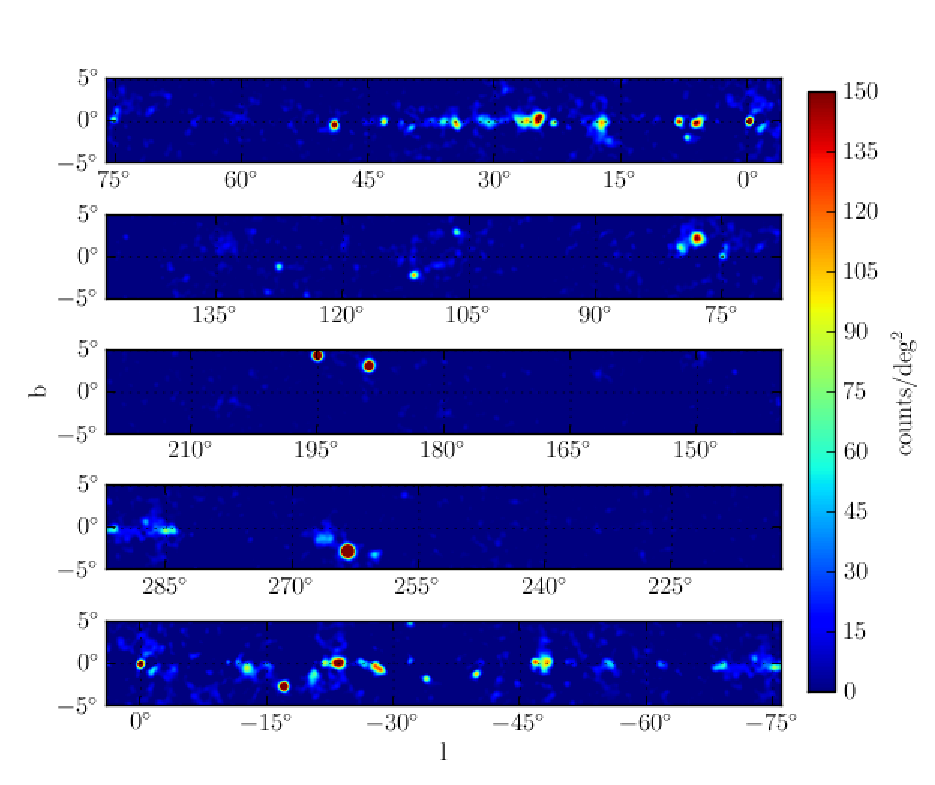
\includegraphics[width=\textwidth]{figures/Plan_gal.eps}
\caption{Residual counts map of the Galactic Plane above 10 GeV. The Galactic and isotropic diffuse emission are subtracted using the files described in section 4.2 with a normalization of 1. All sources associated to Blazars are subtracted using the spectral parameters listed in the hard source list \citep{1FHL}. Excesses visible in this map are due either to Galactic sources or to Blazars not yet associated, emitting above 10 GeV observed by the LAT. The counts map is smoothed with a Gaussian of 0.27$\degr$.
\label{fig:PlanGal}}
\end{figure}

\begin{figure}[h!]
\centering
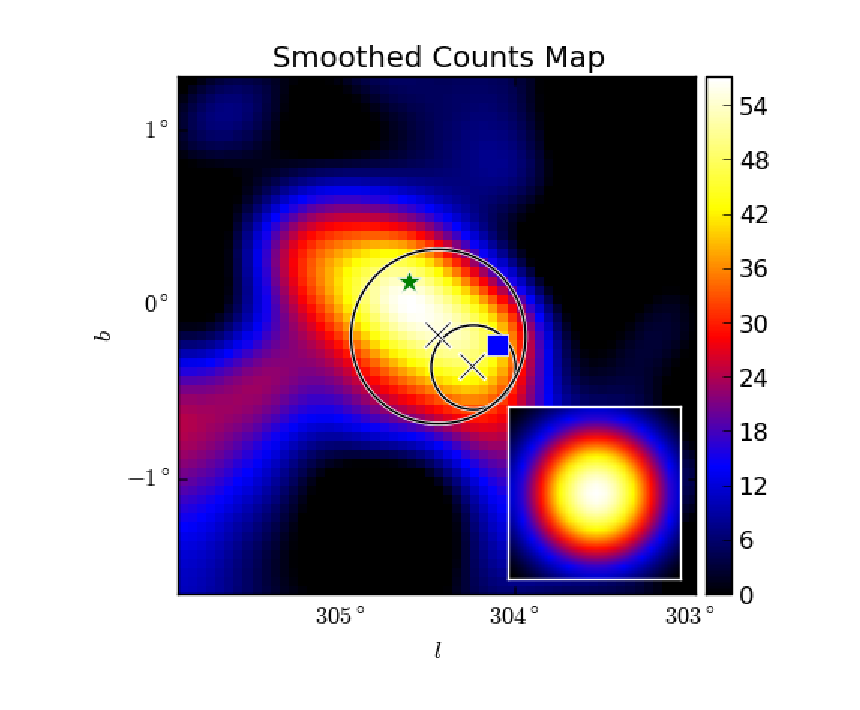
\includegraphics[]{figures/HESSJ1303m631.eps}
\caption{Counts map of the region of HESS~J1303--631. We subtracted the Galactic and isotropic diffuse emission. The counts map is smoothed by a Gaussian of 0.27$\degr$ corresponding to the PSF above 10 GeV. The green star indicates the position of the SNR Kes 17, the blue square represents the position of PSR~J1301--6305. The small and big circles respectively show the extension of the TeV Gaussian proposed by \cite{2005AA...439.1013A} and the extension of the disk derived in this work.
\label{1303}}
\end{figure}

\begin{figure}[h!]
\centering
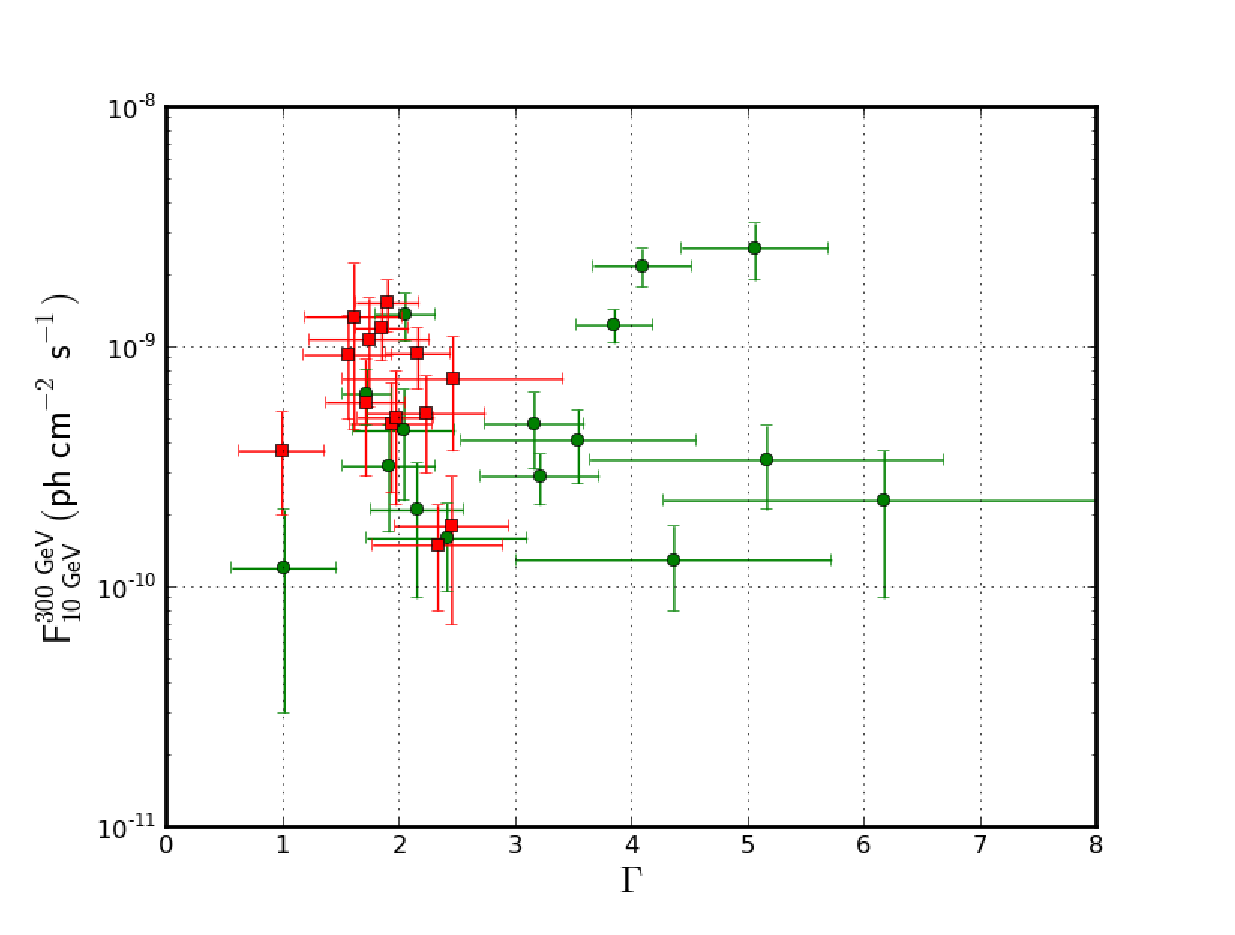
\includegraphics[width=\textwidth]{figures/out_errorbar_best_fit.eps}
\caption{Integrated flux of the detected sources as a function of the power-law index between 10 and 316 GeV (see Table \ref{tab:det_sources}). The green circles show the sources within 0.5$\degr$ of a pulsar detected by the LAT while the red squares represent the sources with no pulsar detected in the GeV energy range within 0.5$\degr$. The error bars show the statistical and systematic uncertainties added in quadrature.  
\label{fig:fluxvssize}}
\end{figure}

\begin{figure}[h!]
\centering
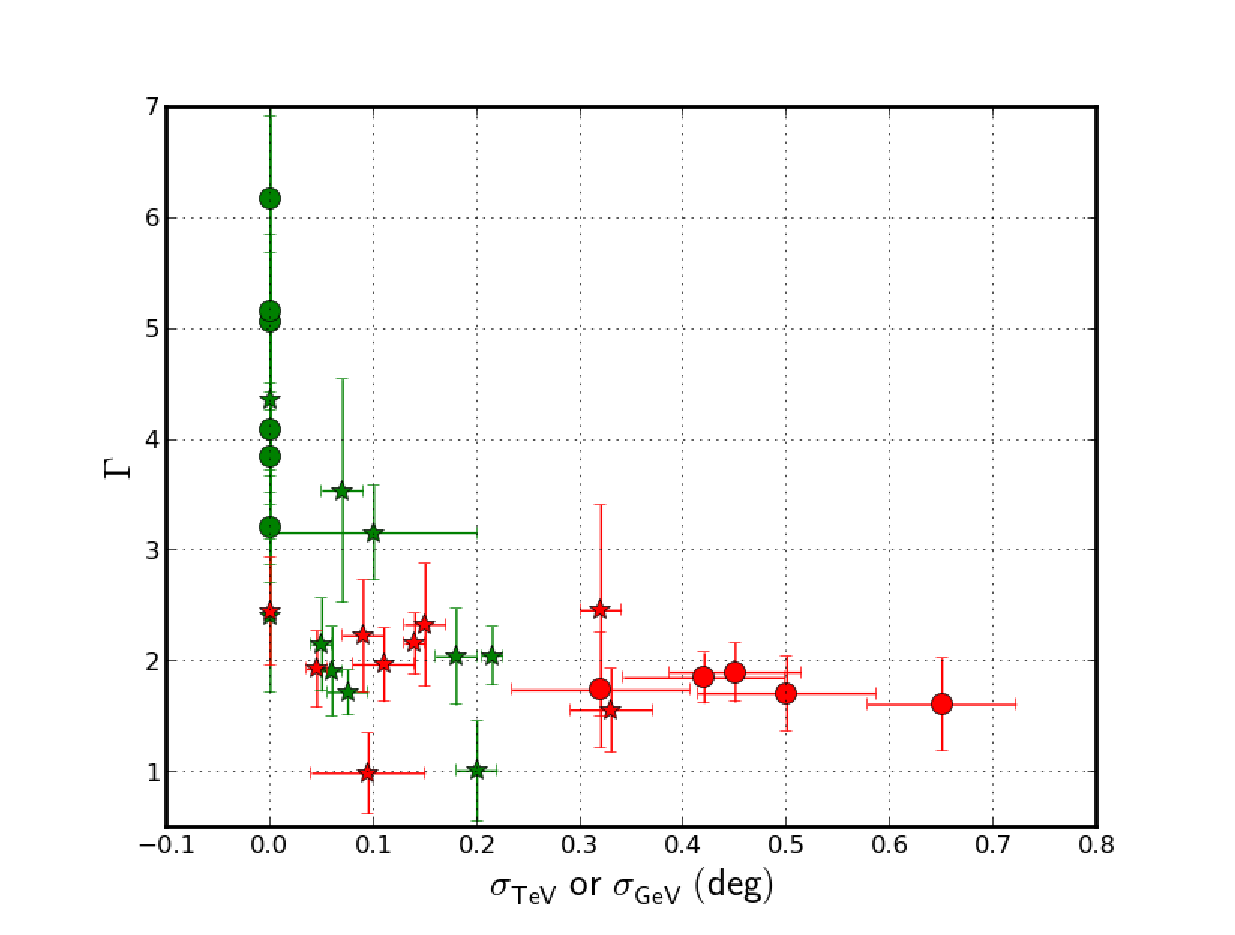
\includegraphics[width=\textwidth]{figures/index_vs_size.eps}
\caption{Spectral index as a function of the GeV or TeV extension for each detected source. The GeV morphology is obtained by fitting the position and extension of the sources as explained in Section \ref{spatanalysis} \& \ref{signi}. The green markers show the sources within 0.5$\degr$ of a pulsar detected by the LAT while the red markers represent the sources with no pulsar detected in the GeV energy range within 0.5$\degr$. The error bars show the statistical and systematic uncertainties added in quadrature. The 11 circles represent the sources for which the GeV morphology significantly improved the fit compared to the TeV morphology (Table \ref{tab:GeVmorph}), while the stars represent the sources modeled assuming their TeV morphology. For sources modelled assuming their TeV morphology, we reported the uncertainties found in the associated reference in Table \ref{tab:TeV_sources}. For asymmetric sources we represented the mean extension with an error bar corresponding to the maximum uncertainty.
\label{fig:indexvssize}}
\end{figure}

%\begin{figure}[h!]
%\centering
%\includegraphics[width=0.5\textwidth]{figures/0FGLJ1958.12848.eps}
%\caption{SED of MGRO J1958$+$2848. The red and blue points show respectively the \emph{Fermi}-LAT and ... points. The black error bars show the statistical and   systematic uncertainties added in quadrature. The black line corresponds to the best fit obtained using the LAT data. The dashed line correspond to the model of PSR J... taken from \cite{2012ApJS..199...31N}.
%\label{fig:1}}
%\end{figure}


\begin{figure}[h!]
\centering
\subfigure{
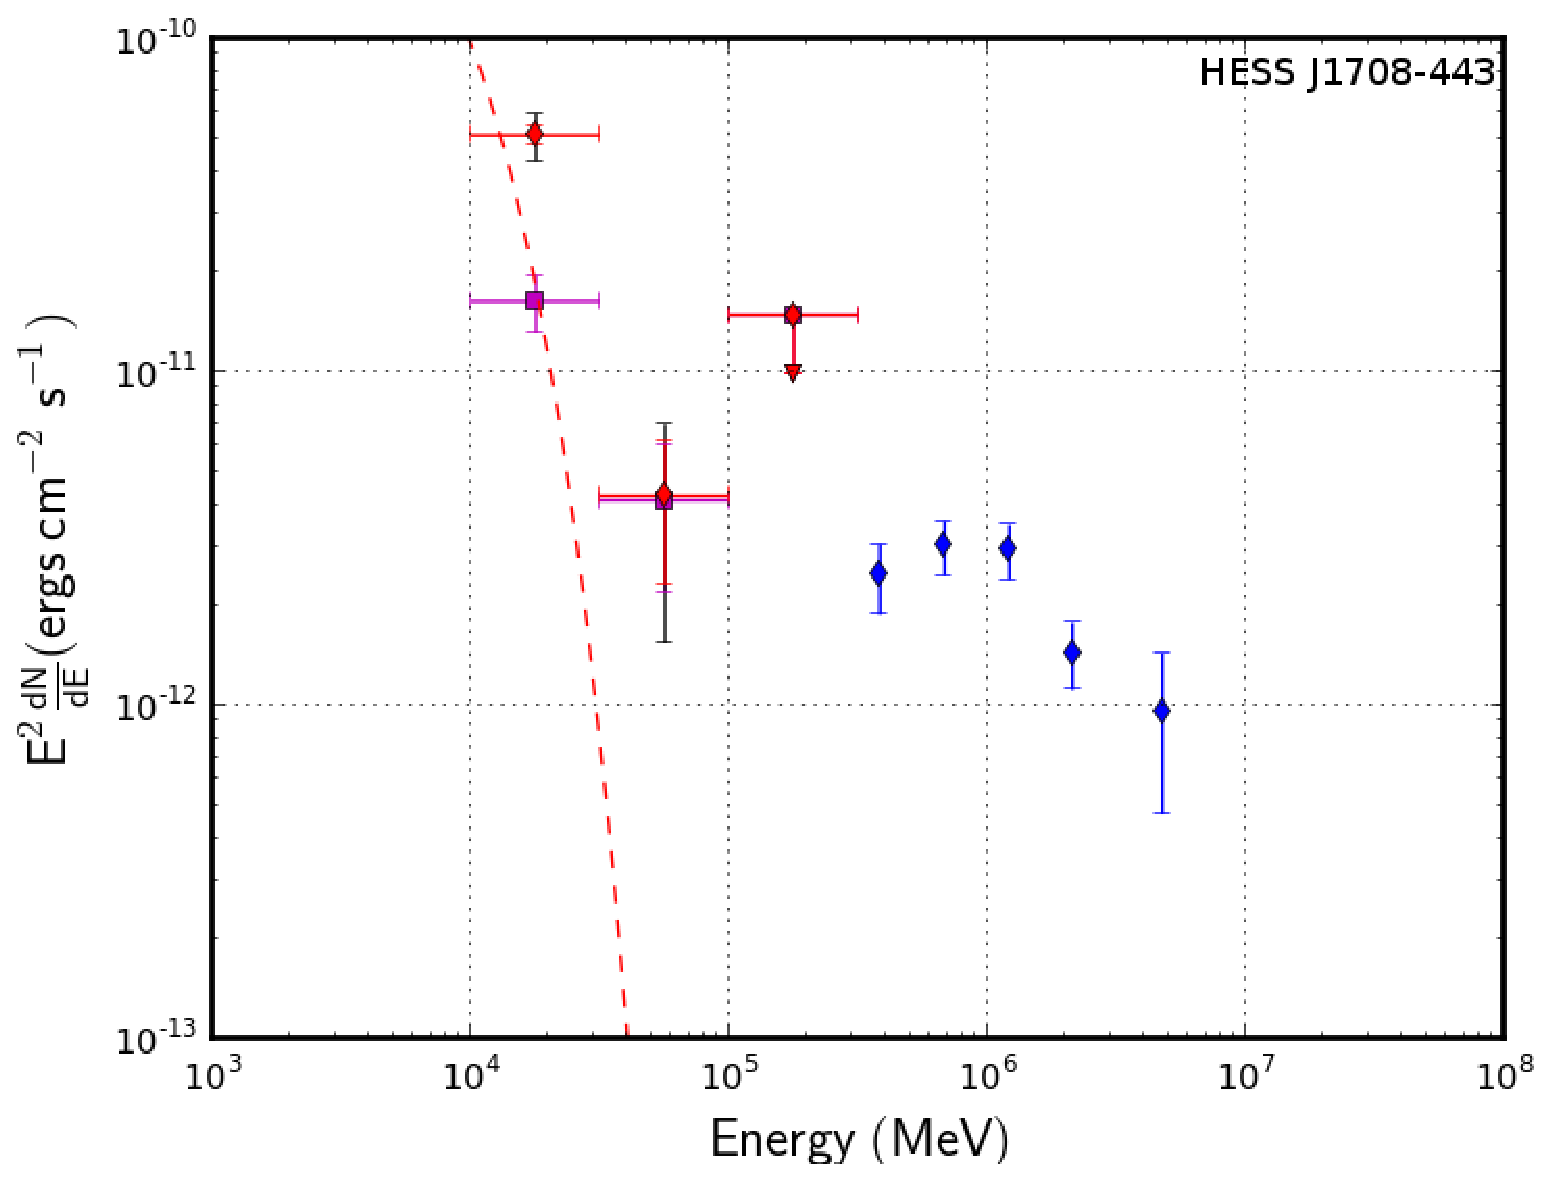
\includegraphics[width=0.45\textwidth]{figures/HESSJ1708.eps}
\label{fig:hess1708}
}
\subfigure{
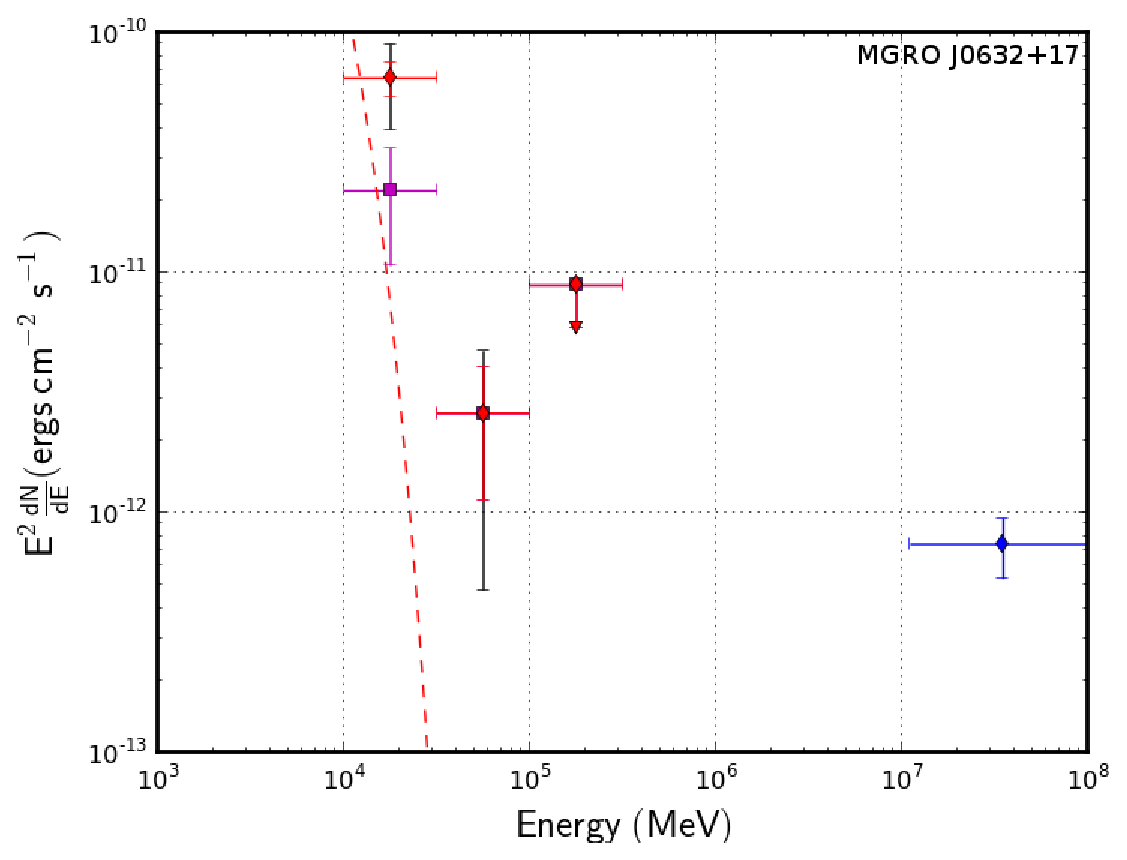
\includegraphics[width=0.45\textwidth]{figures/MGROJ0632.eps}
\label{fig:mgroj0632}
}
\subfigure{
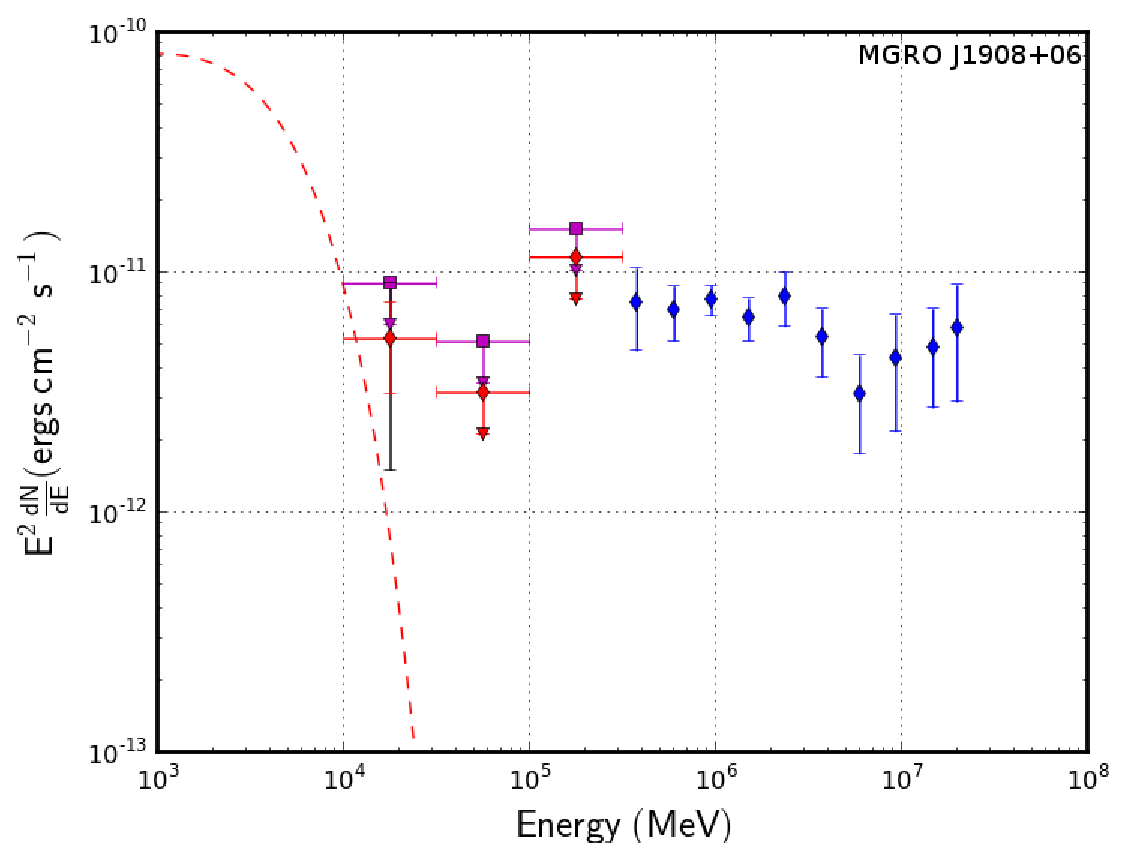
\includegraphics[width=0.45\textwidth]{figures/MGROJ1908.eps}
\label{fig:mgro1908}
}
\subfigure{
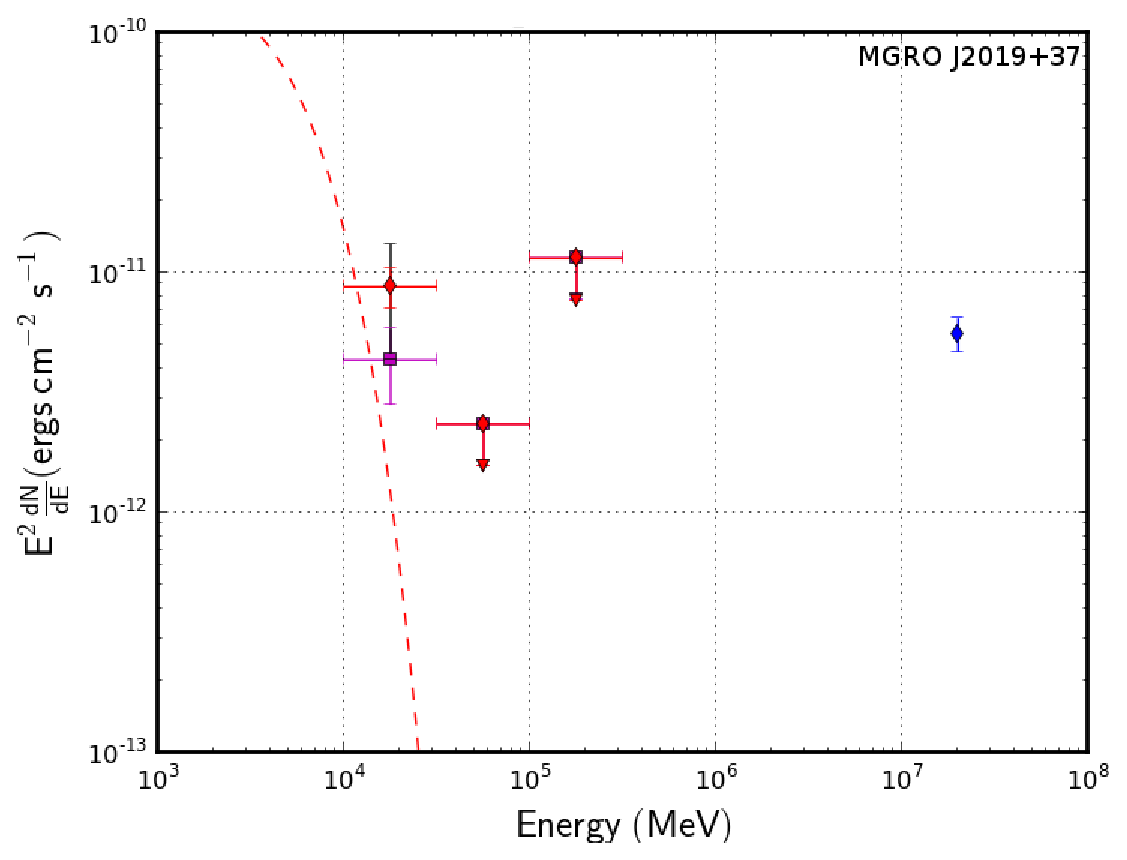
\includegraphics[width=0.45\textwidth]{figures/MGROJ201937.eps}
\label{fig:mgro2019}
}
\subfigure{
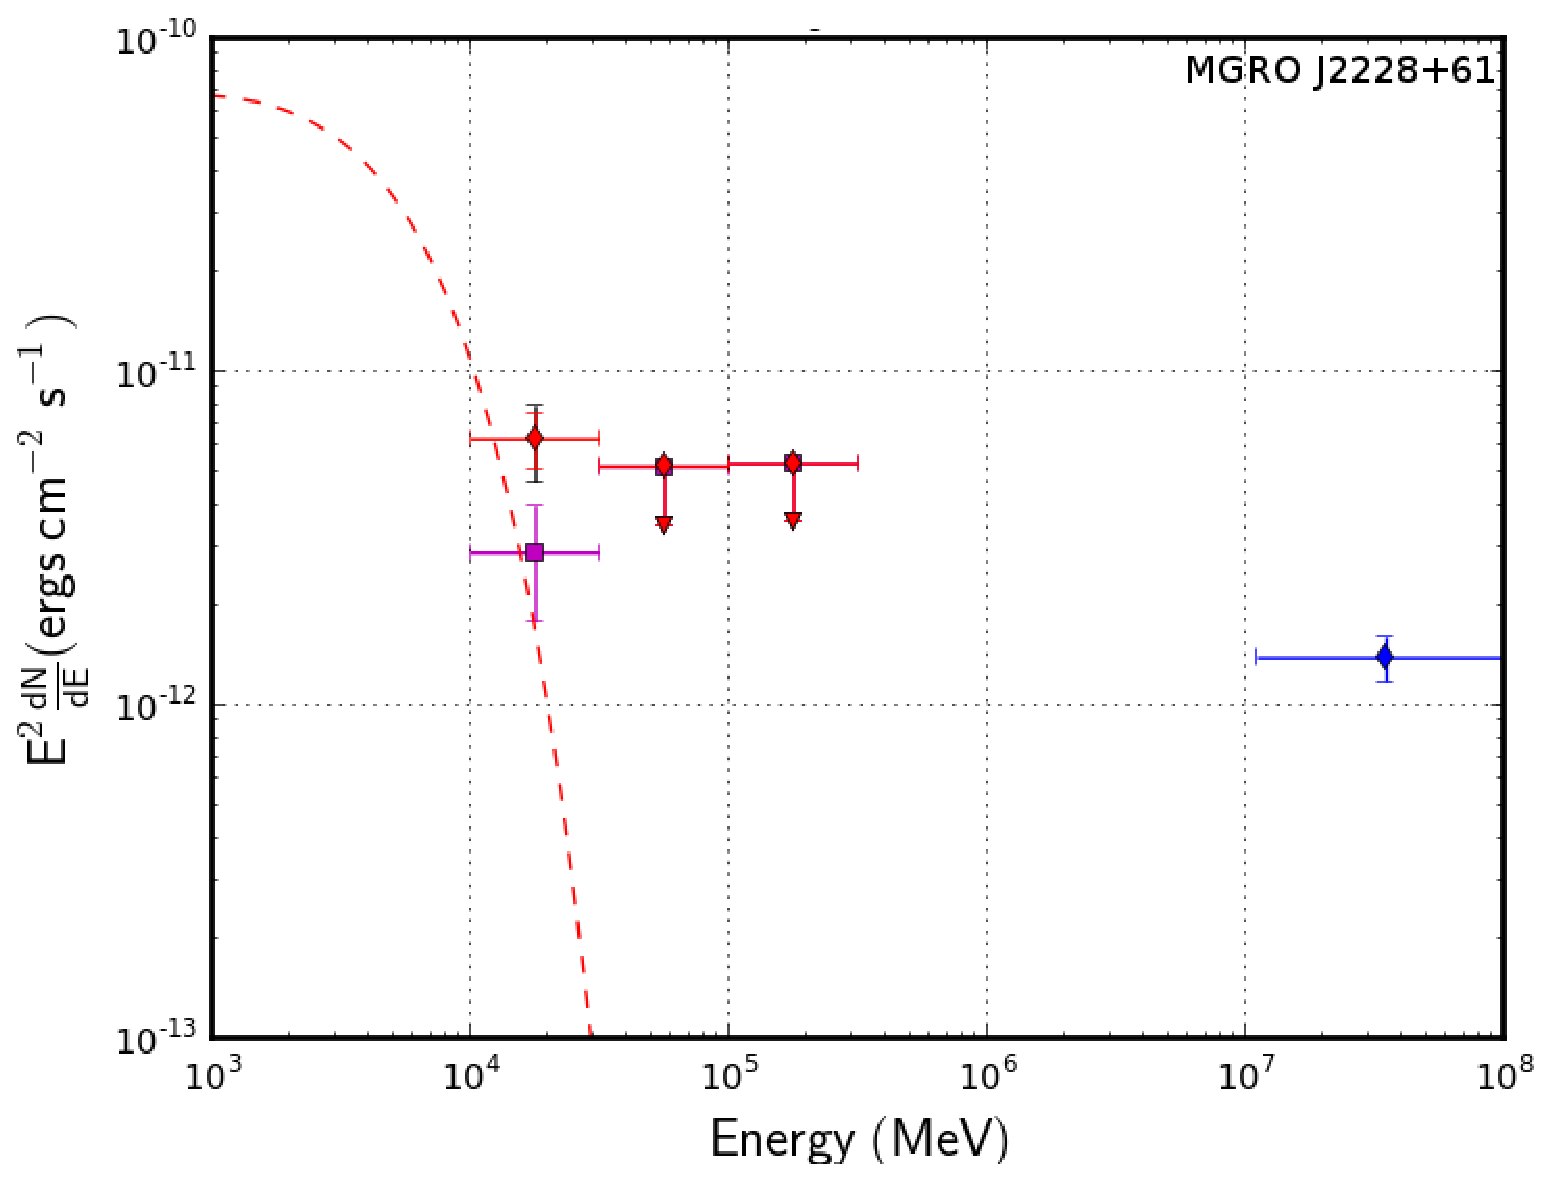
\includegraphics[width=0.45\textwidth]{figures/MGROJ2228.eps}
\label{fig:mgroj2228}
}
\subfigure{
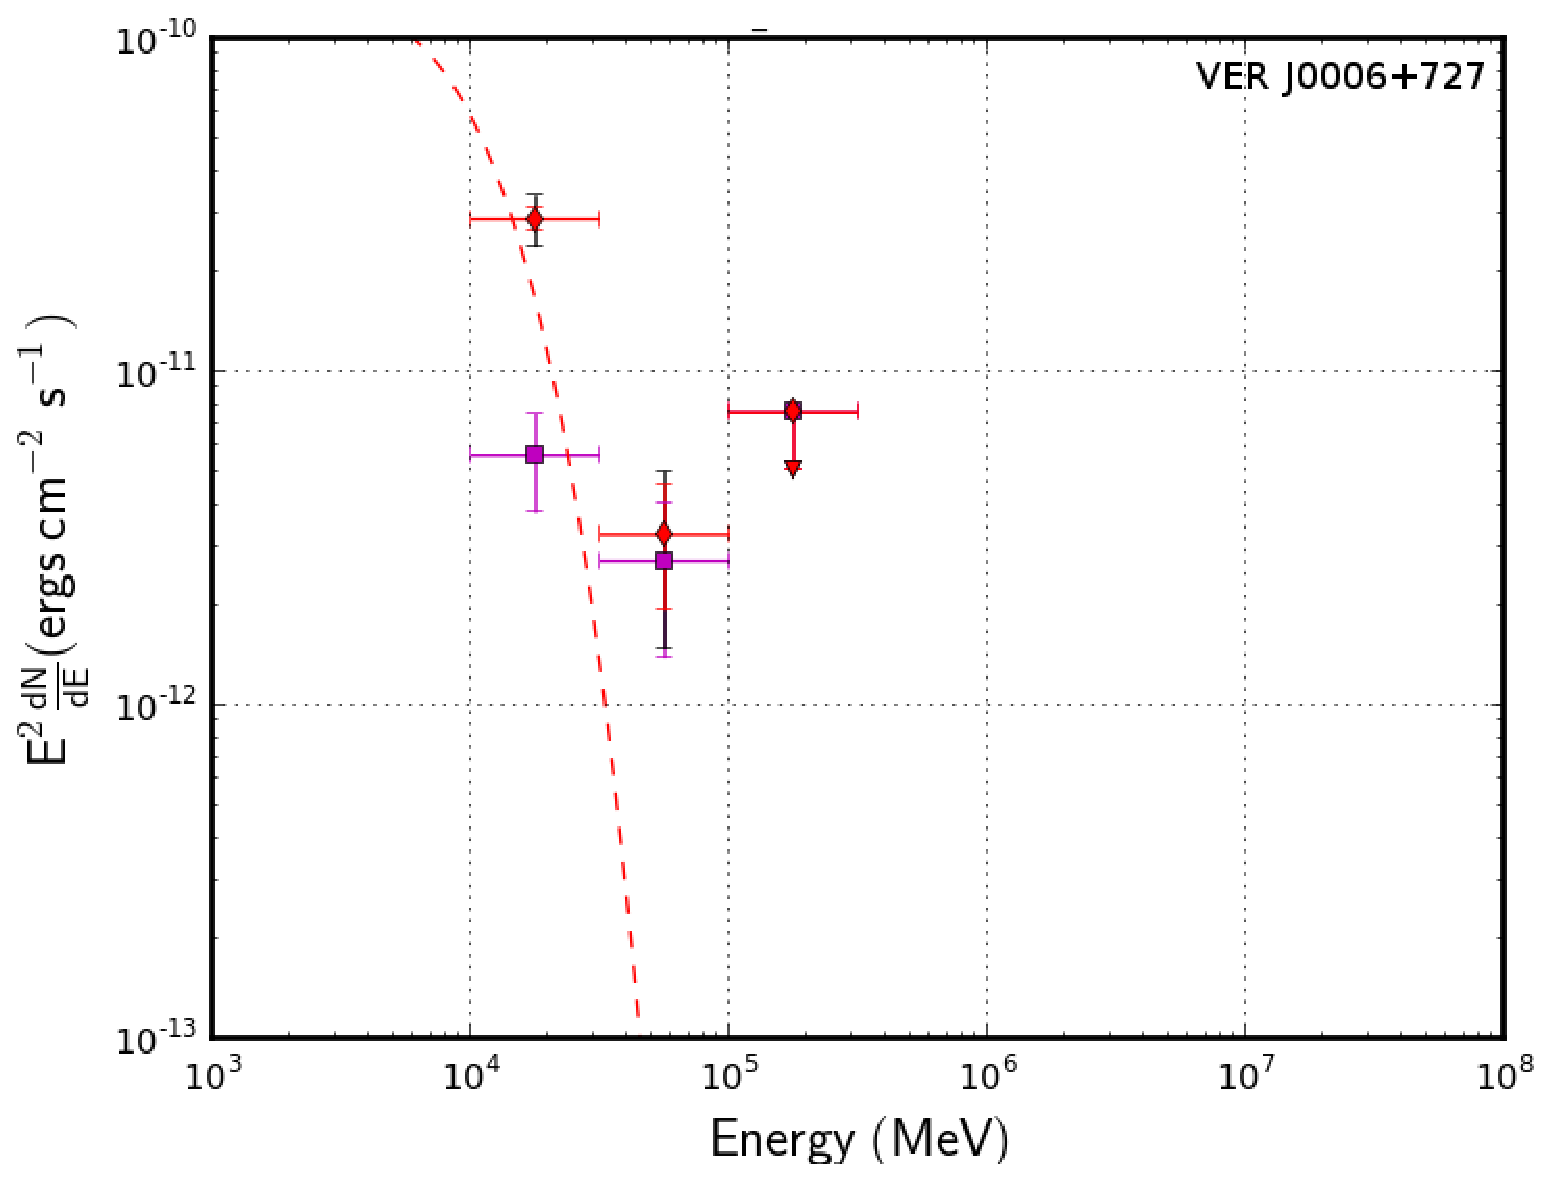
\includegraphics[width=0.45\textwidth]{figures/VERJ0006.eps}
\label{fig:verj0006}
}
\caption{\label{fig:sedsourcespuls}SED of sources better described by a point-like source and with a pulsar within 0.5$\degr$. The blue points show the TeV points taken from \cite{2011AA...528A.143H, 2009ApJ...700L.127A, 2009AA...499..723A, 2007ApJ...664L..91A, 2009ApJ...700L.127A, 2011arXiv1111.2591M}. The red circles and the magenta squares show respectively the SED without the pulsar included in the model and with the pulsar included in the model. The black error bars show the statistical and   systematic uncertainties added in quadrature. The dashed line corresponds to the model of the associated pulsars sumarized in Table \ref{tab:pulsarfit}. In the case of MGRO J1908+06, the red SED was derived assuming a point-like source as determined in Table \ref{tab:GeVmorph} while the magenta SED was derived assuming the TeV shape since it is not significant anymore when the pulsar is included in the model.}
\end{figure}

\begin{figure}[h!]
\centering
\subfigure{
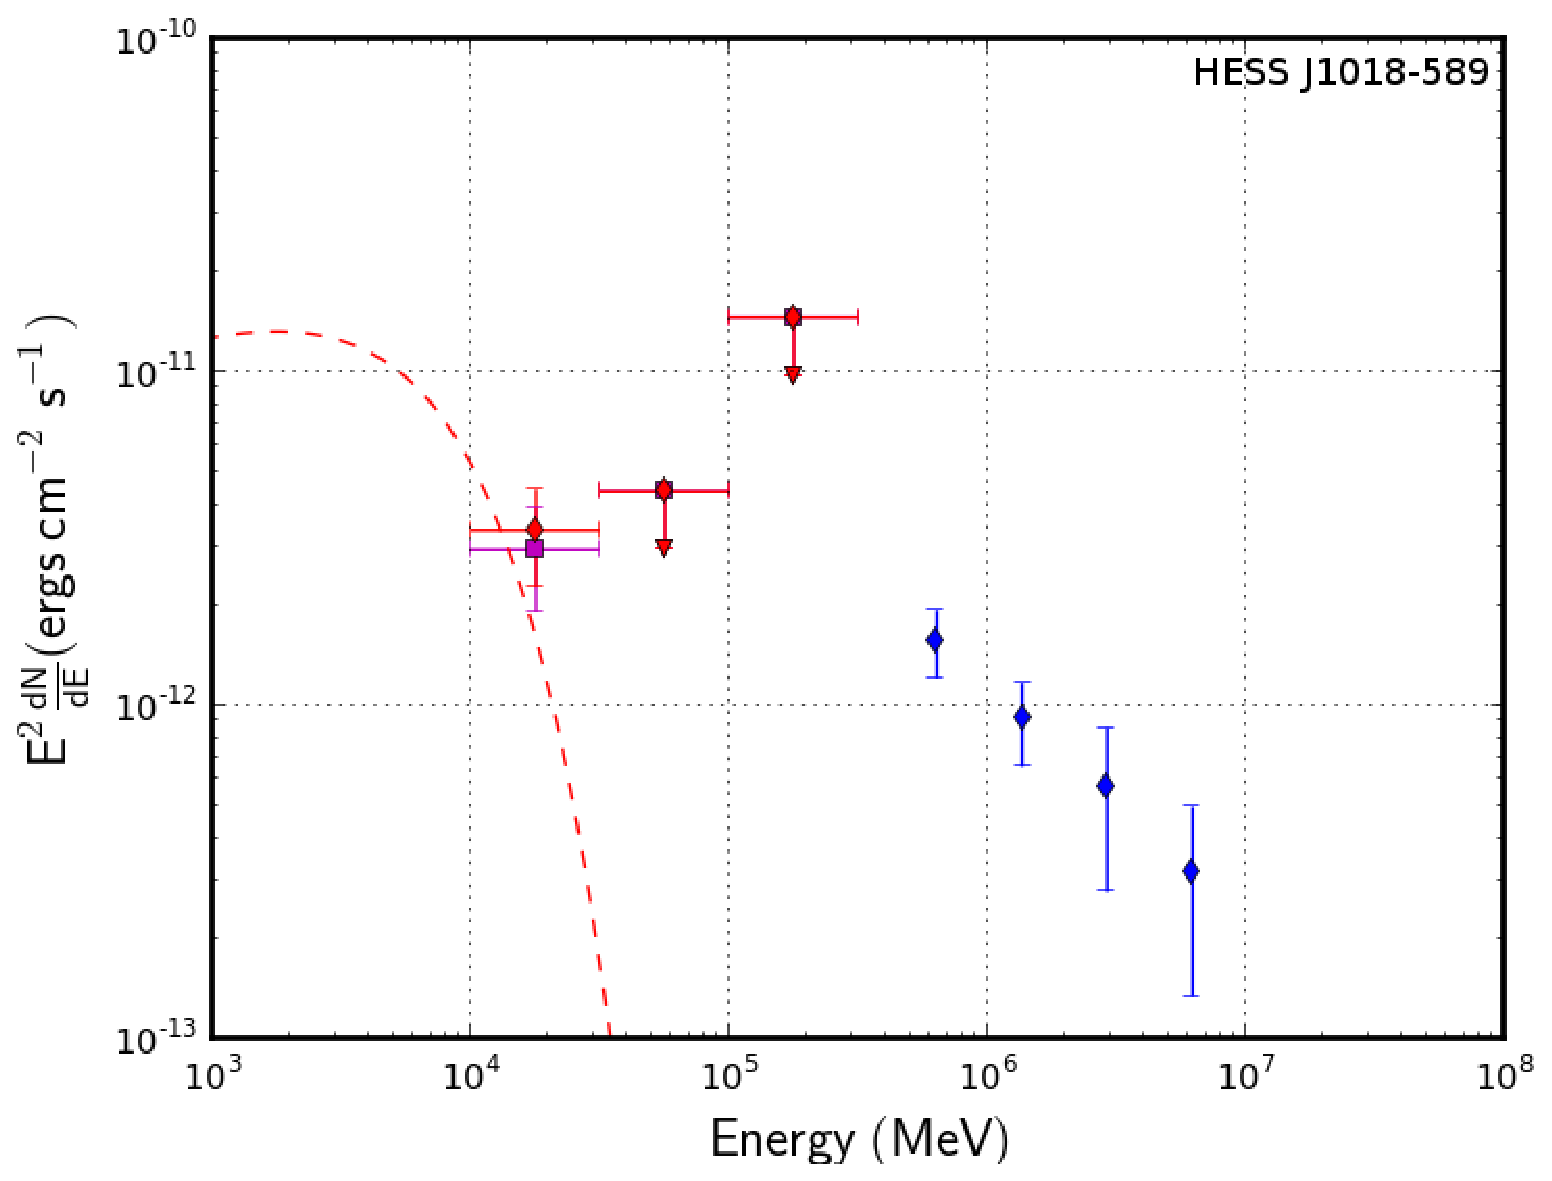
\includegraphics[width=0.45\textwidth]{figures/HESSJ1018.eps}
\label{fig:hessj1018}
}
\subfigure{
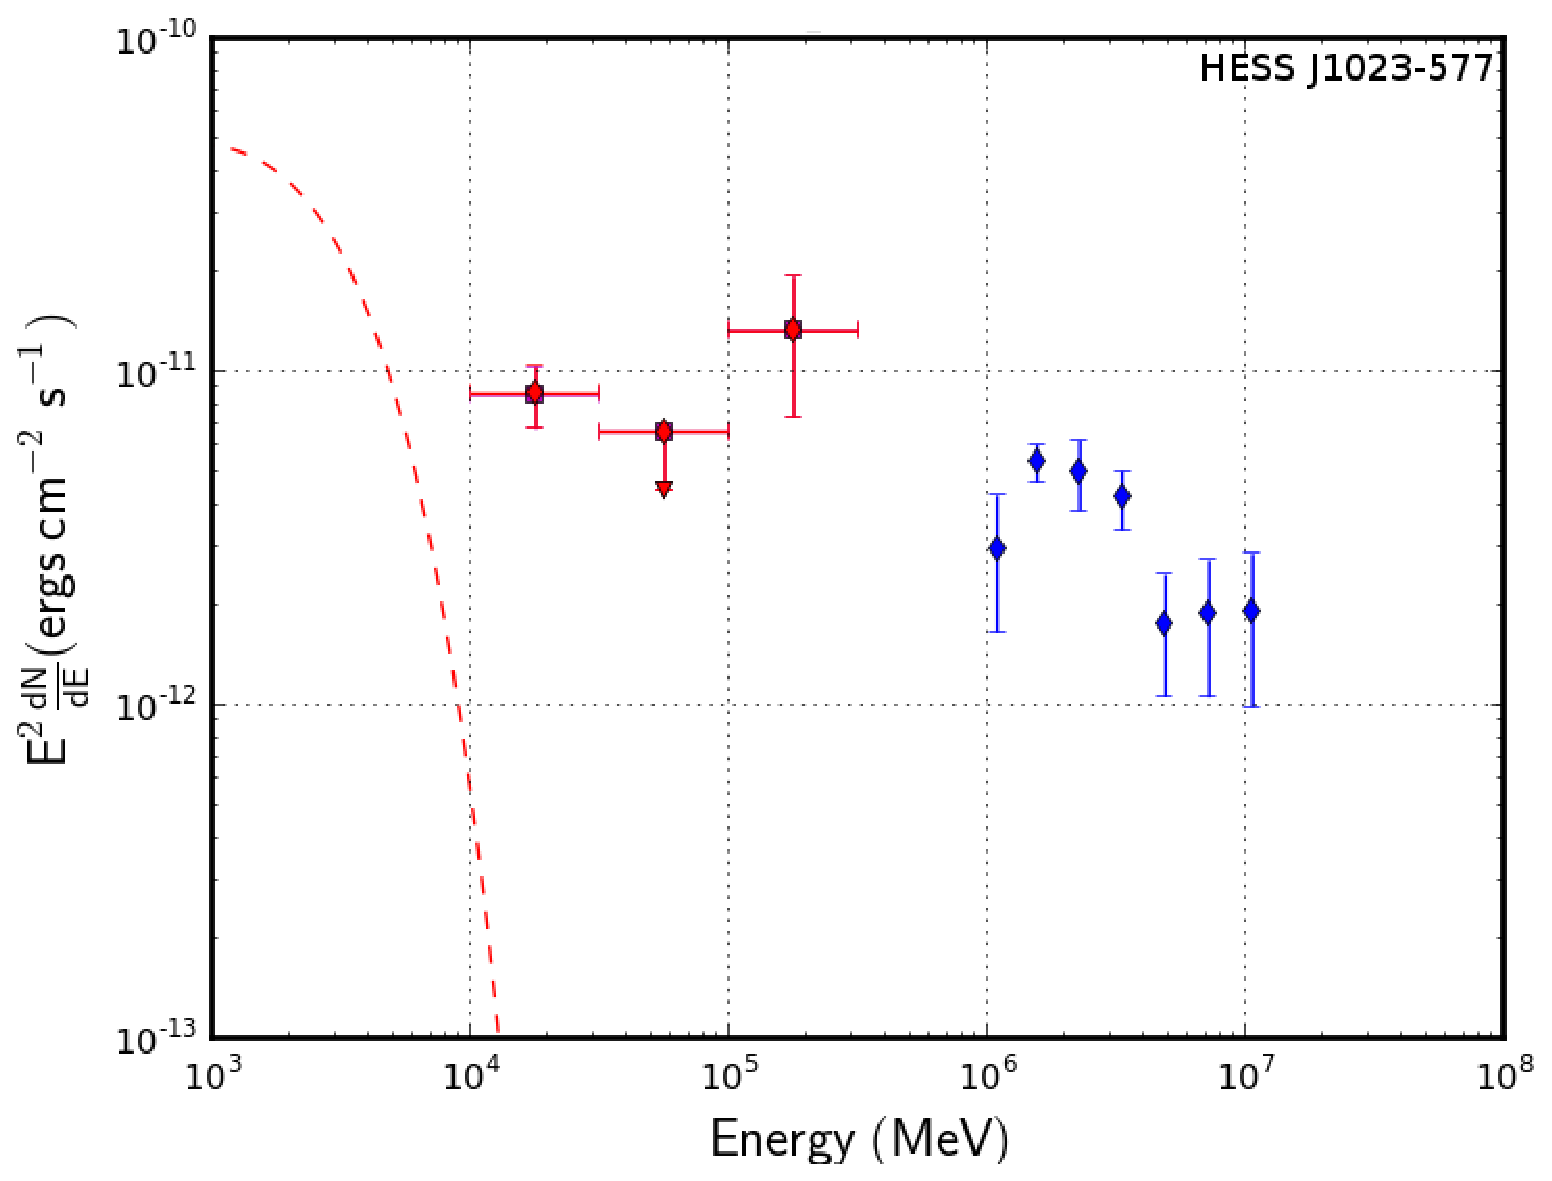
\includegraphics[width=0.45\textwidth]{figures/HESSJ1023.eps}
\label{fig:hessj1023}
}
\subfigure{
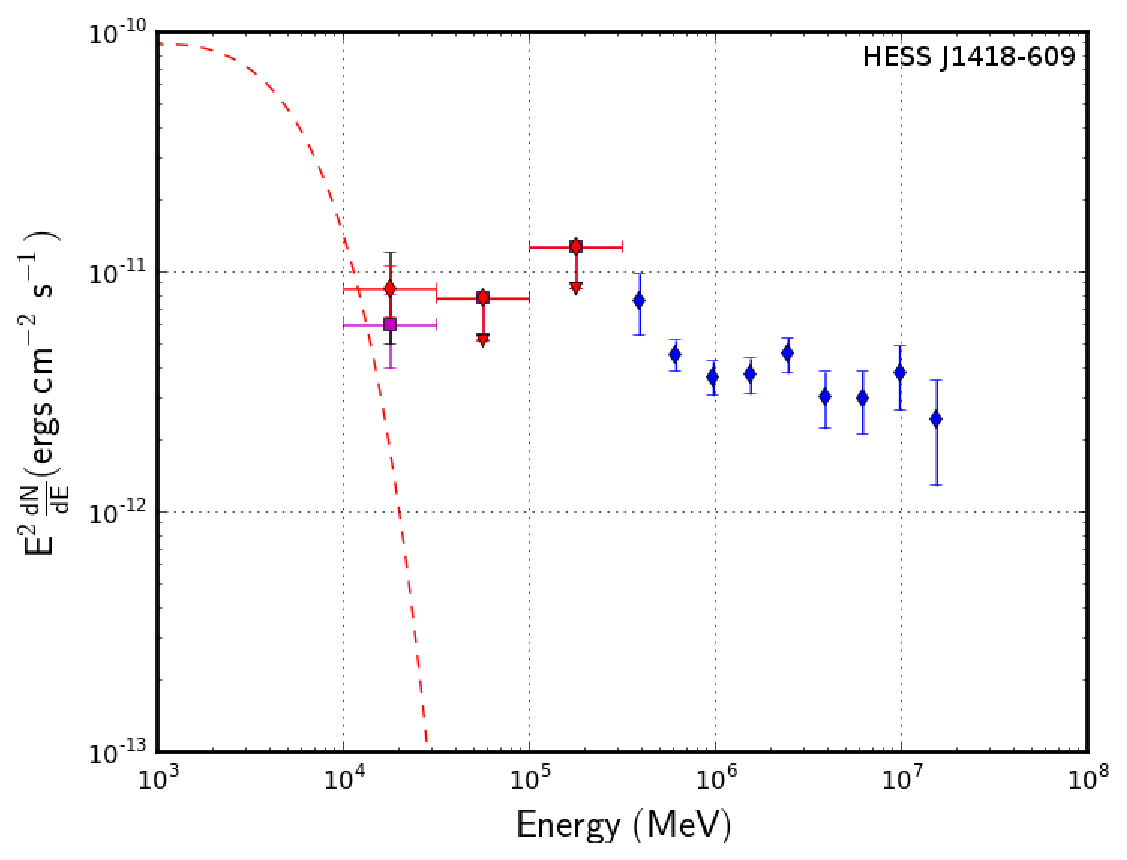
\includegraphics[width=0.45\textwidth]{figures/HESSJ1418.eps}
\label{fig:hessj1418}
}
\subfigure{
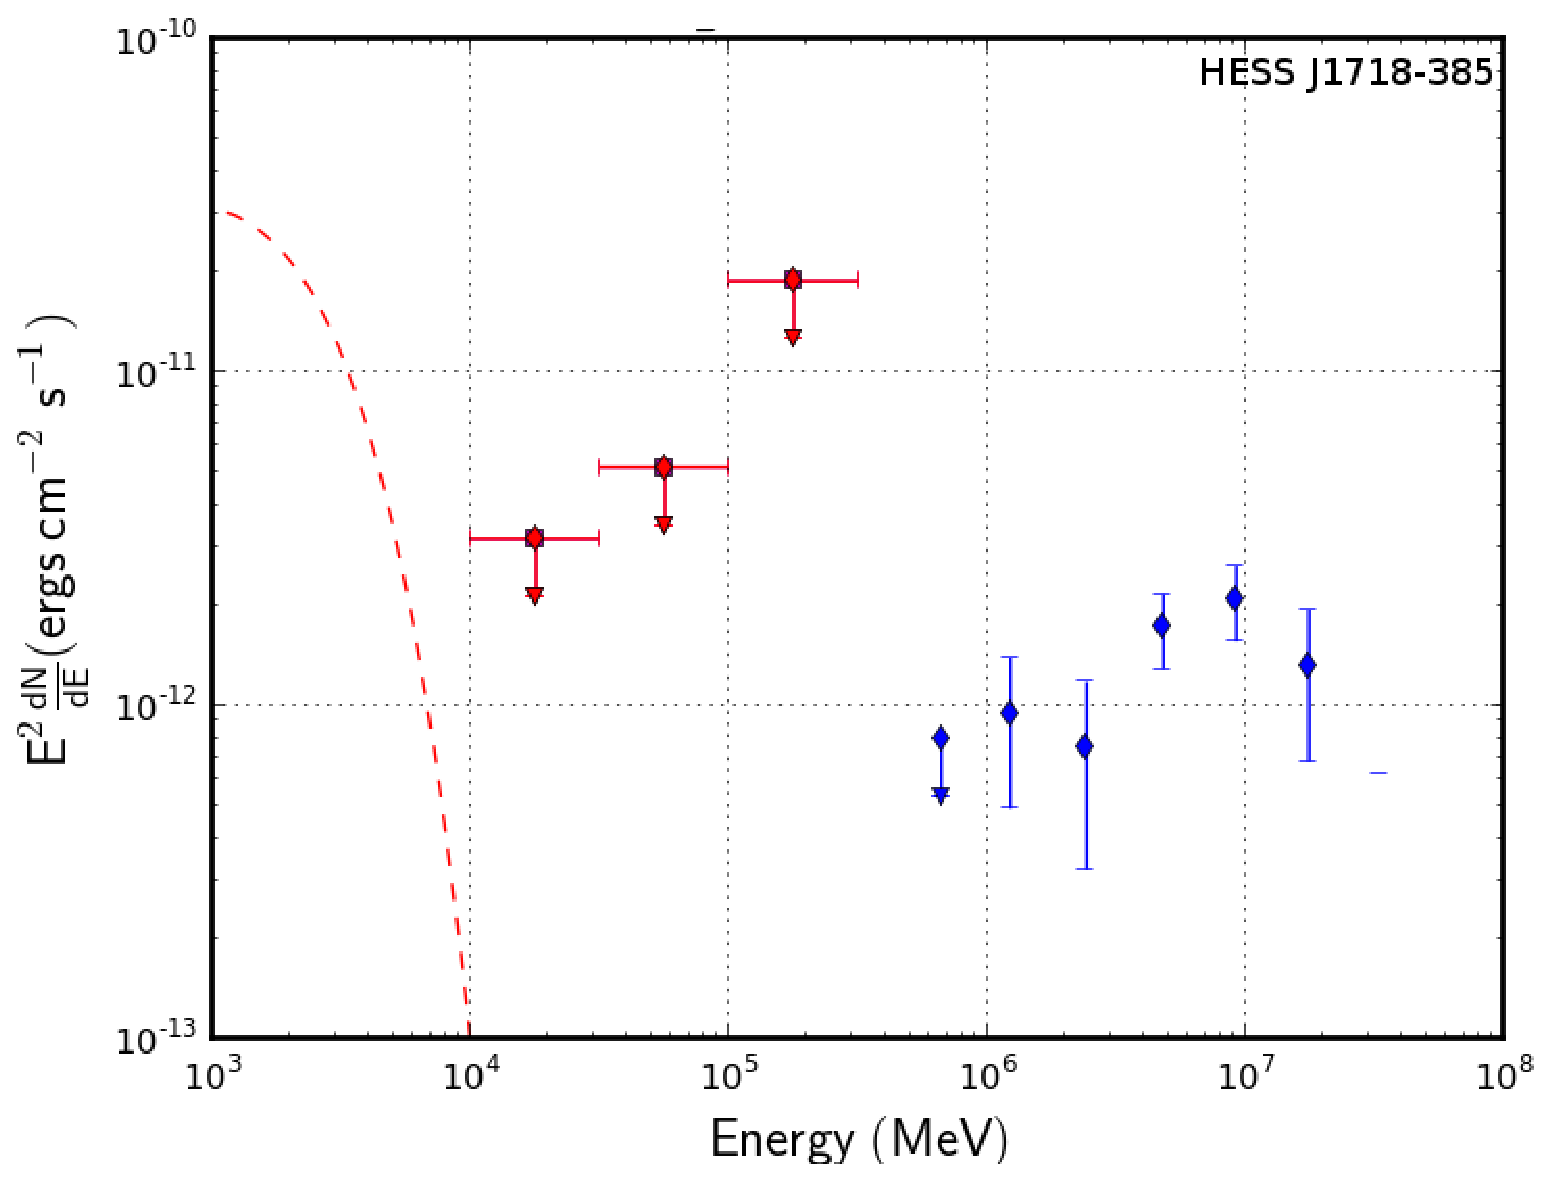
\includegraphics[width=0.45\textwidth]{figures/HESSJ1718.eps}
\label{fig:hessj1718}
}
\caption{\label{fig:sedsourcespuls2}SED of sources better described by the TeV shape and with a pulsar within 0.5$\degr$. The blue points show the TeV points taken from the associated paper in Table \ref{tab:TeV_sources}. The red circles and the magenta squares show respectively the SED without the pulsar included in the model and with the pulsar included in the model. The black error bars show the statistical and   systematic uncertainties added in quadrature. The dashed line corresponds to the model of the associated pulsars sumarized in Table \ref{tab:pulsarfit}.}
\end{figure}

\begin{figure}[h!]
\centering

\subfigure{
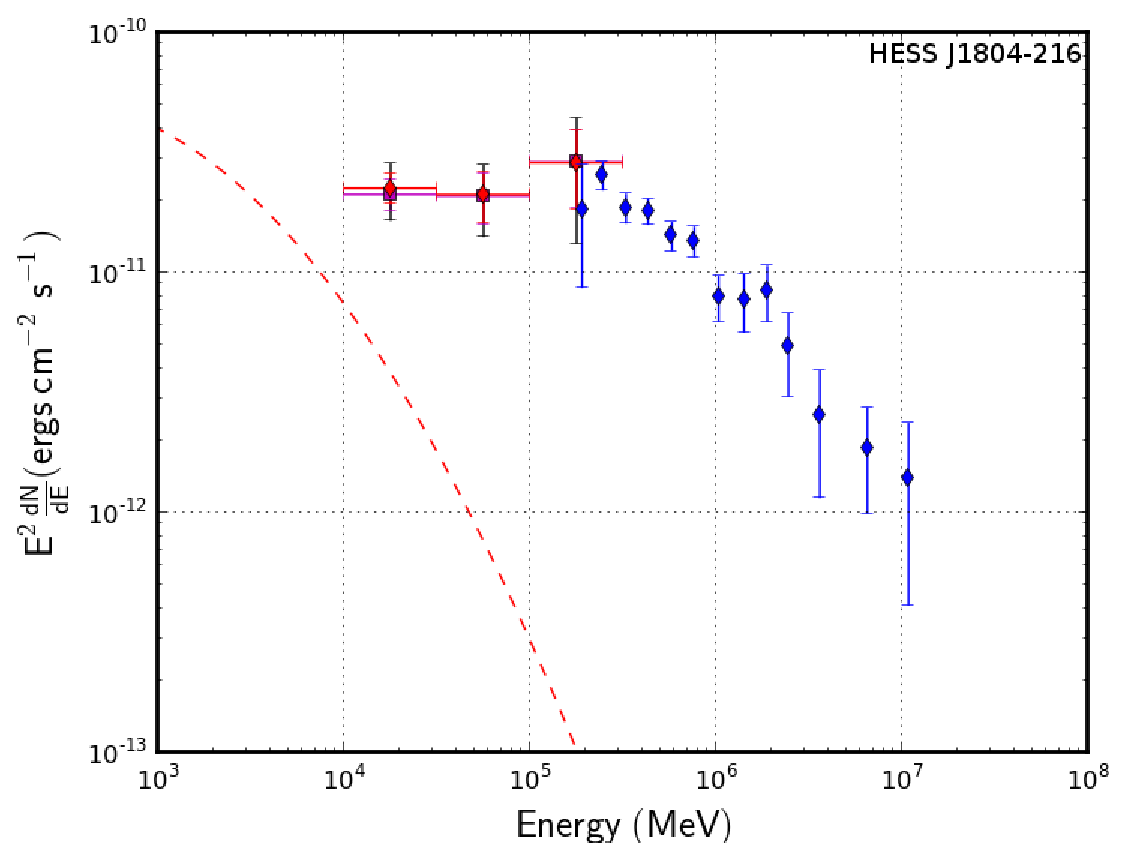
\includegraphics[width=0.45\textwidth]{figures/HESSJ1804.eps}
\label{fig:hessj1804}
}
\subfigure{
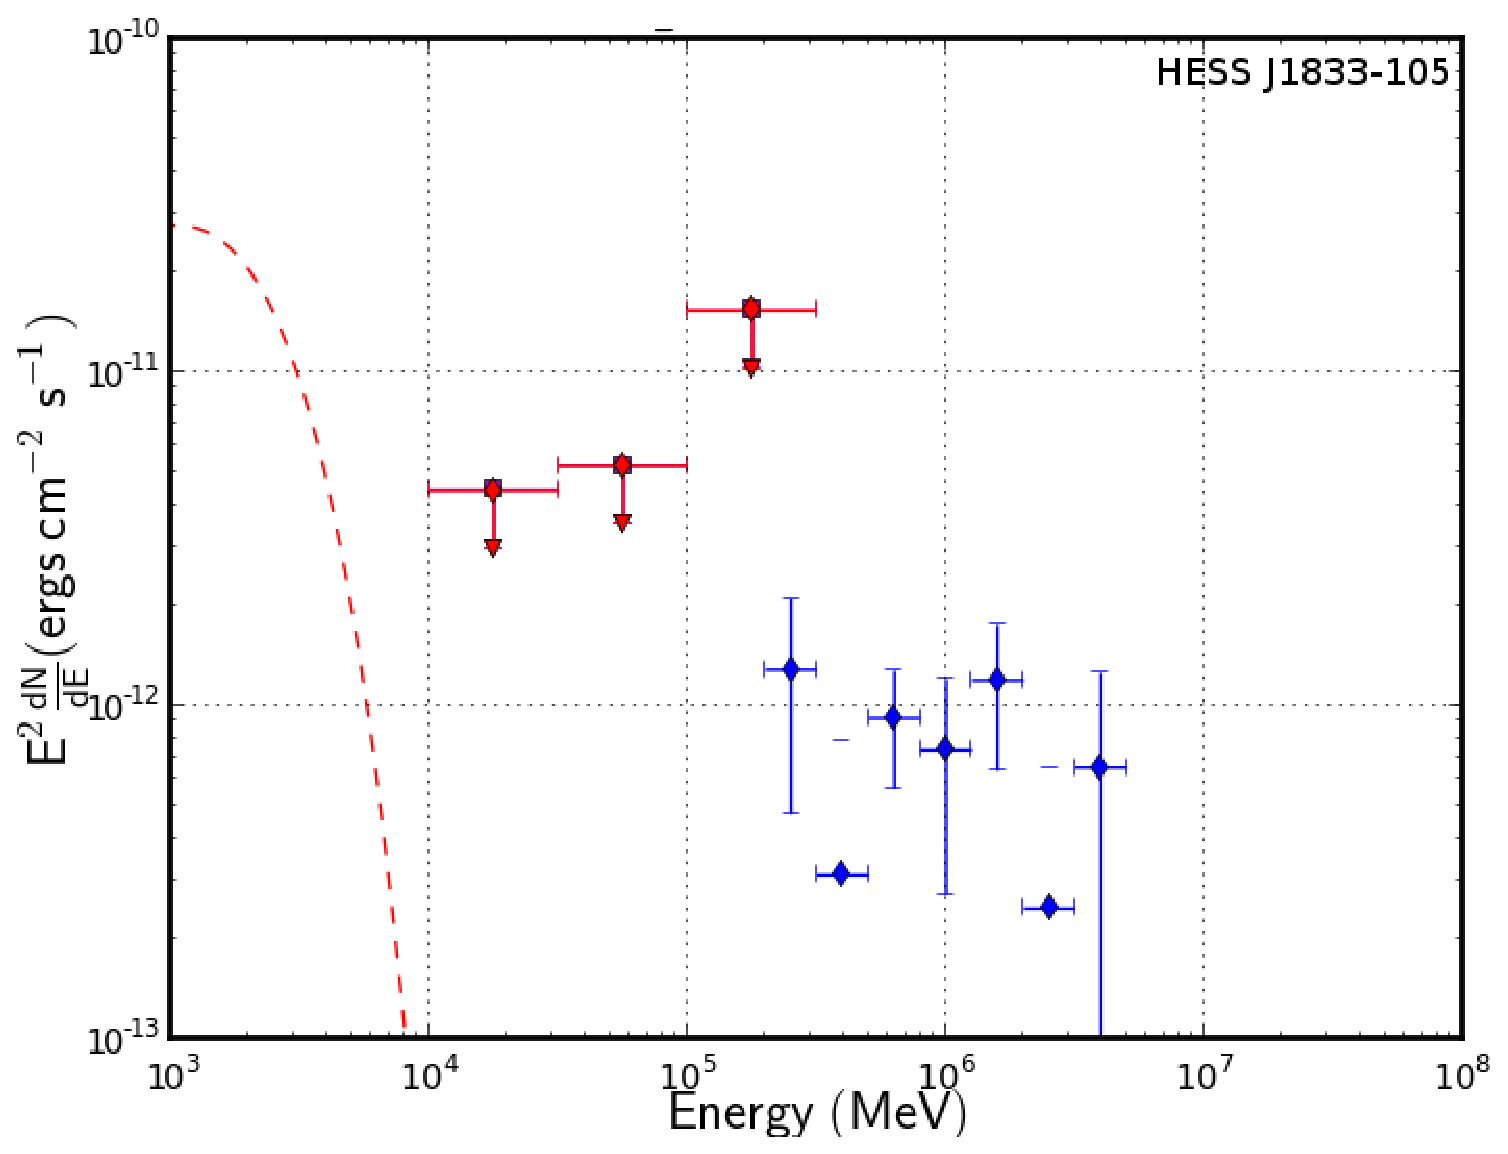
\includegraphics[width=0.45\textwidth]{figures/HESSJ1833.eps}
\label{fig:hess1833}
}
\subfigure{
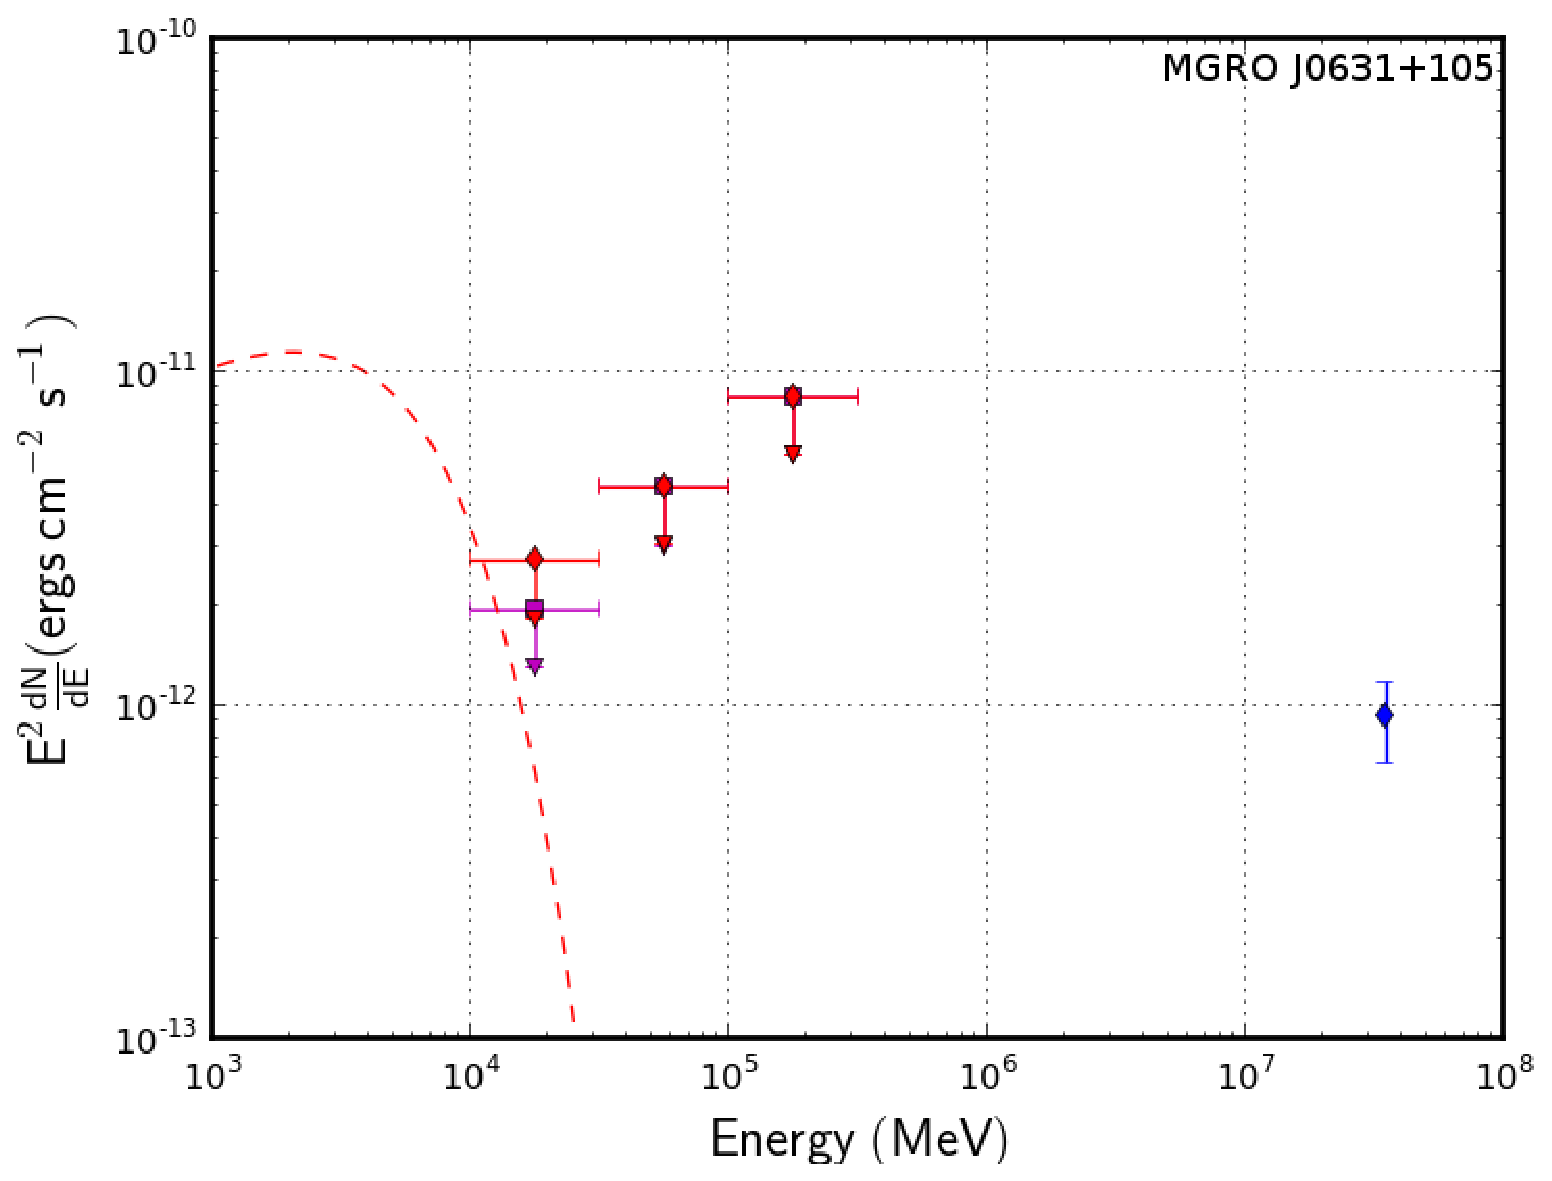
\includegraphics[width=0.45\textwidth]{figures/MGROJ0631.eps}
\label{fig:mgroj0631}
}
\subfigure{
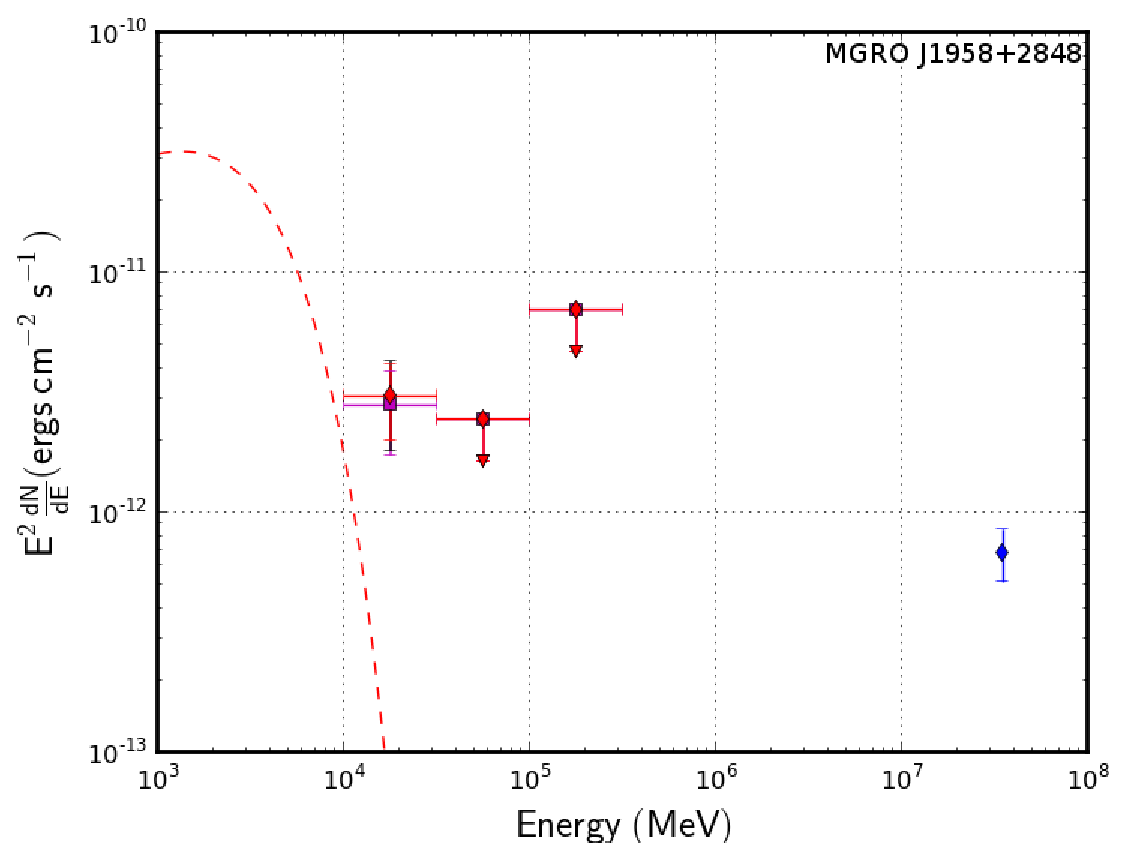
\includegraphics[width=0.45\textwidth]{figures/MGROJ1958.eps}
\label{fig:mgroj1958}
}

\caption{\label{fig:sedsourcespuls3}SED of sources better described by the TeV shape and with a pulsar within 0.5$\degr$. The blue points show the TeV points taken from the associated paper in Table \ref{tab:TeV_sources}. The red circles and the magenta squares show respectively the SED without the pulsar included in the model and with the pulsar included in the model. The black error bars show the statistical and   systematic uncertainties added in quadrature. The dashed line corresponds to the model of the associated pulsars summarized in Table. \ref{tab:pulsarfit}.}
\end{figure}

\clearpage

\begin{figure}[h!]
\centering
\subfigure{
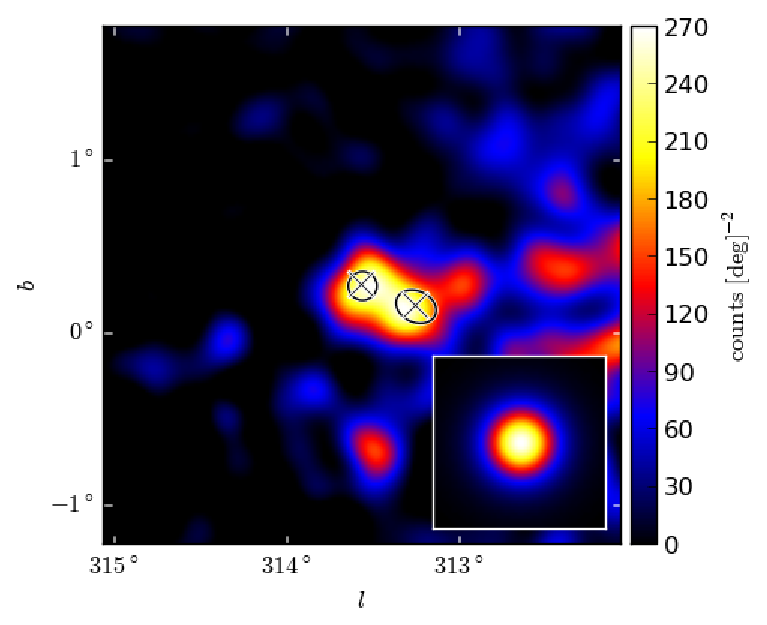
\includegraphics[width=0.60\textwidth]{figures/K310GeV.eps}}
\subfigure{
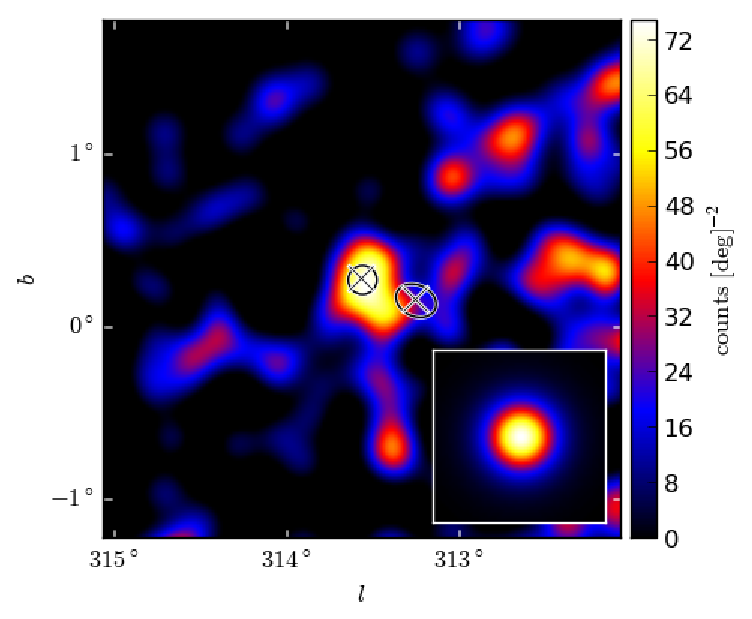
\includegraphics[width=0.60\textwidth]{figures/K330GeV.eps}}
\caption{Smoothed counts map of the region of the Kookaburra complex observed by Fermi above 10 GeV (Top) and
30 GeV (Bottom). The Galactic diffuse emission is subtracted. The circle and right ellipse show the best fit obtained in TeV respectively for the K3 nebula and the Rabbit nebula.
\label{fig:K3countsmap}}
\end{figure}

\clearpage

\begin{figure}[h!]
\centering
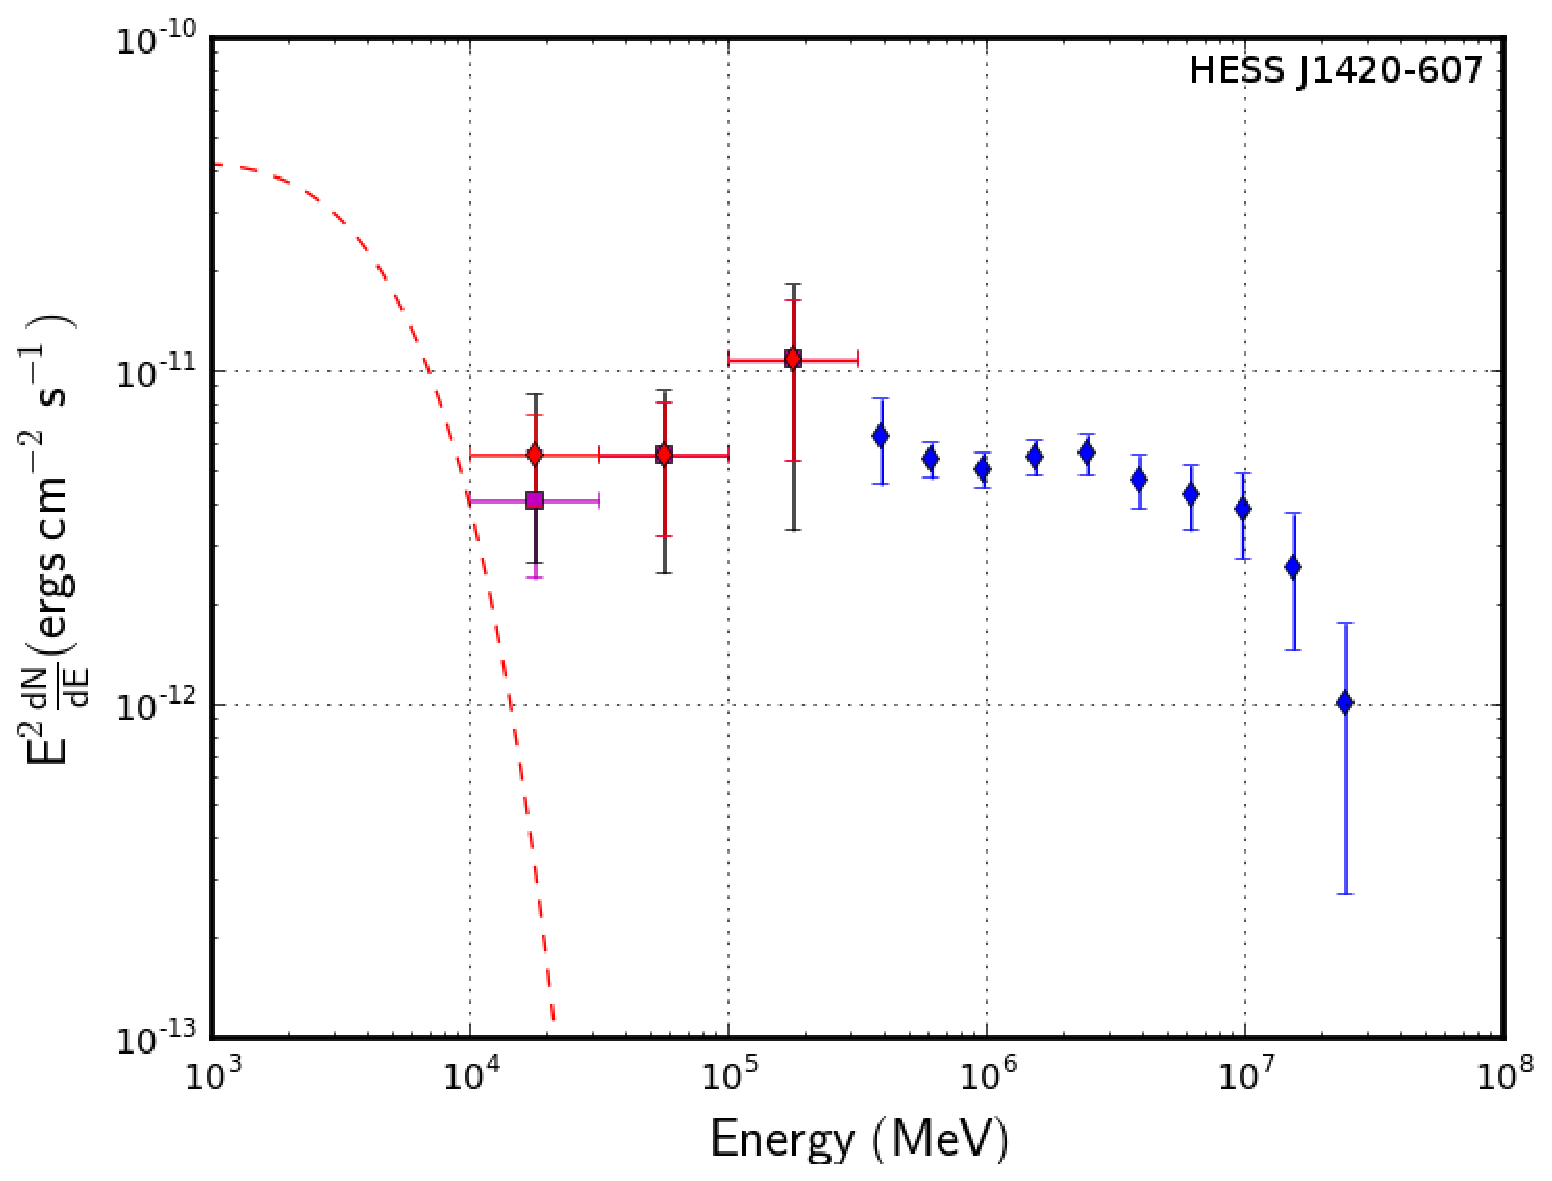
\includegraphics[width=0.60\textwidth]{figures/HESSJ1420.eps}
\caption{SED of HESS J1420-607. The blue, green and magenta points respectively show the spectral points obtained by HESS \citep{2006AA...456..245A}, by Suzaku \citep{2010ApJ...711.1168V} and the upper limits derived in radio. The red points and the magenta squares show the spectral points obtained in this work without and with the pulsar included in the model. In the LAT energy range the black error bars show the statistical and systematic uncertainties added in quadrature. The red dashed line corresponds to the 2FGL spectrum of the PSR J1420-607. The three black lines show the results of SED modeling for the broad extended nebula emission presented in previous works. The solid and dot dashed lines respectively shows to the hadronic plus leptonic and leptonic models proposed by \cite{2010ApJ...711.1168V}. The dotted line corresponds to the leptonic model proposed by \cite{2012ApJ...750..162K} assuming an ambient magnetic field of 3$\mu$G.
\label{fig:hessj1420}}
\end{figure}

\begin{figure}[h!]
\centering
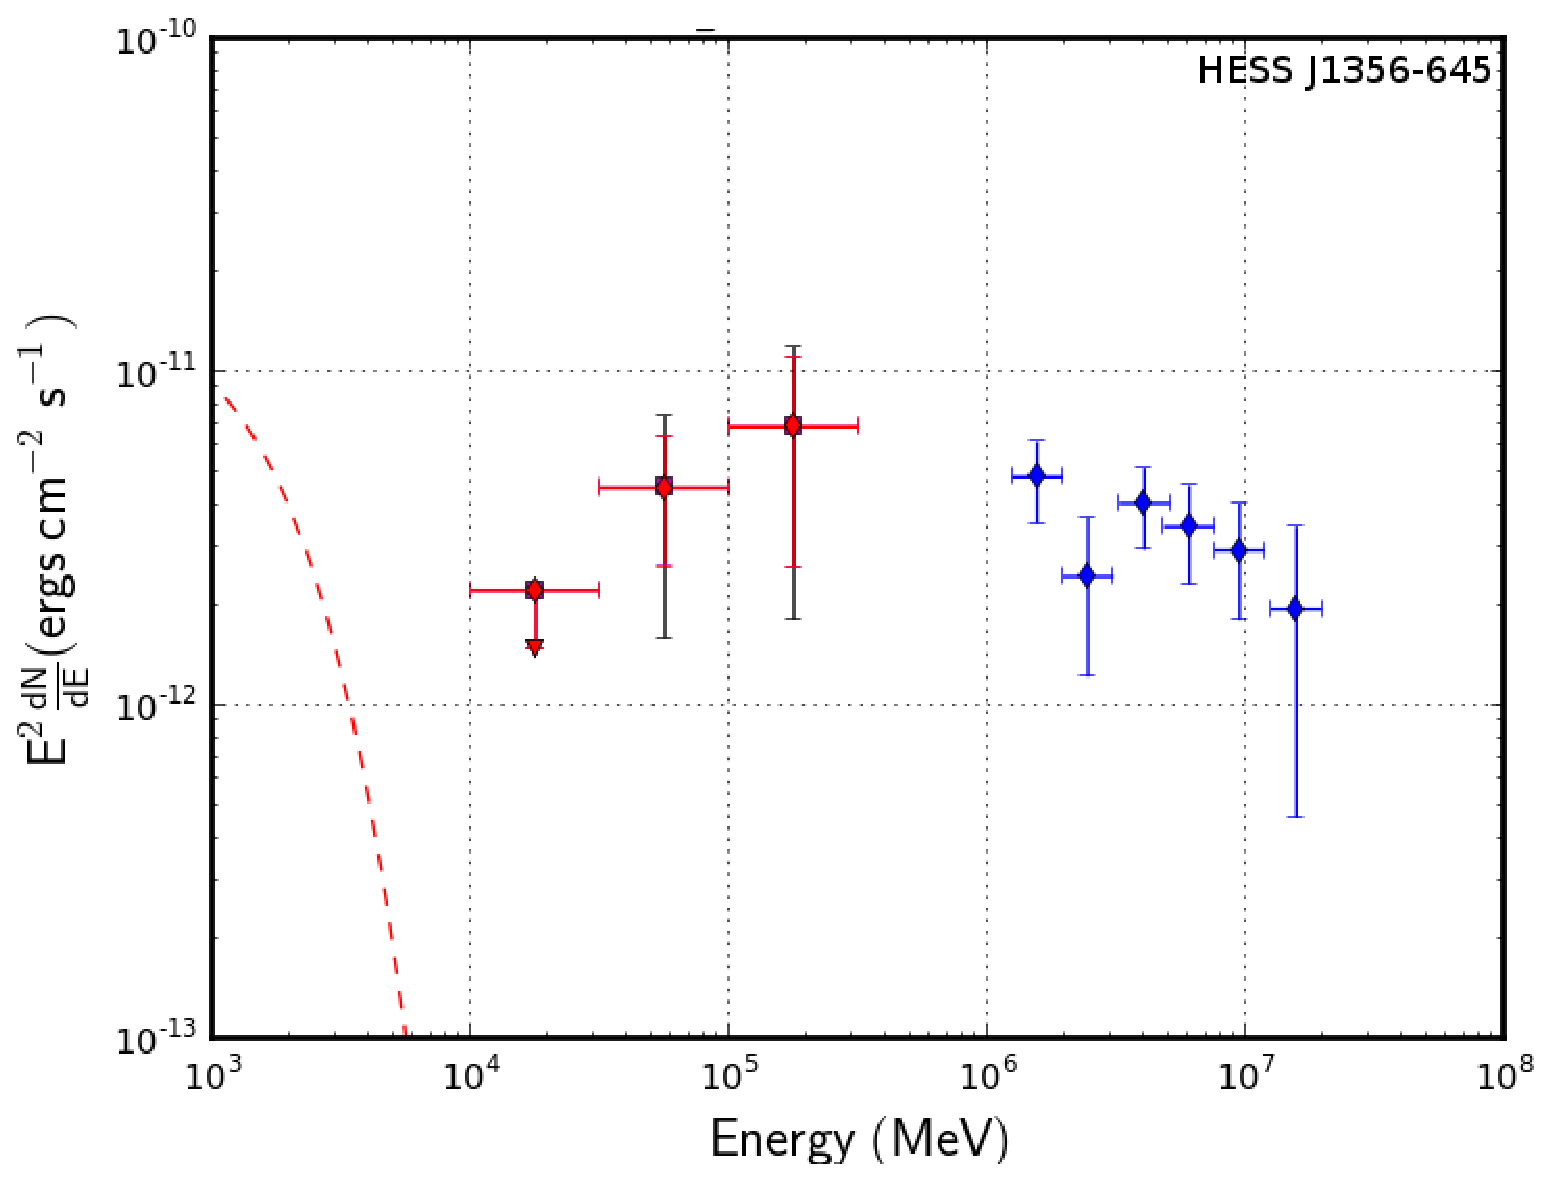
\includegraphics[width=0.60\textwidth]{figures/HESSJ1356.eps}
\caption{SED of HESS J1356-645. The blue, green and magenta points represents the results obtained by HESS \citep{2011AA...533A.103H}, the X-ray data \citep{2011AA...533A.102L} and the radio data \citep{2007MNRAS.382..382M, 1995MNRAS.277...36D, 1993AJ....105.1666G}. The red and magenta points between 10 and 316 GeV show the points obtained in this work without and with PSR J1357-6429 included in the model. In the LAT energy range the red and black error bars respectively show the statistical and systematic uncertainties added in quadrature. The solid line presents the one-zone leptonic model proposed by \cite{2011AA...533A.103H}.
\label{fig:hess1356}}
\end{figure}

\begin{figure}[h!]
\centering
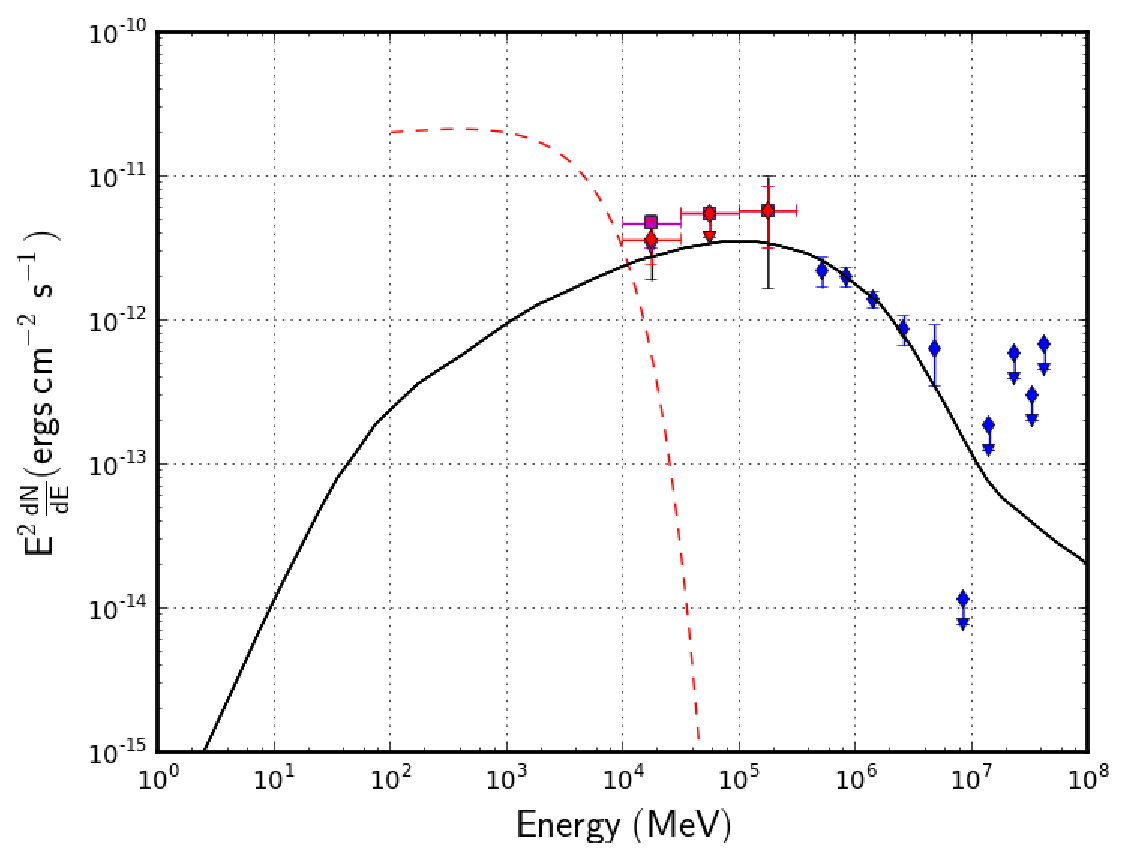
\includegraphics[width=0.60\textwidth]{figures/HESSJ1119.eps}
\caption{SED of HESS J1119$-$614. The blue points represent the HESS data \citep{Mayerdiploma}. The red and magenta points between 10 and 316 GeV show the points obtained in this work without and with PSR J1119$-$6127 included in the model. In the LAT energy range the red and black error bars respectively show the statistical and systematic uncertainties added in quadrature. The solid line shows the model proposed by \cite{Mayerdiploma}. The red dashed line corresponds to the model of PSR~J1119$-$6127 \citep{2012ApJS..199...31N}.
\label{fig:hessj1119}}
\end{figure}



\begin{figure}[h!]
\centering
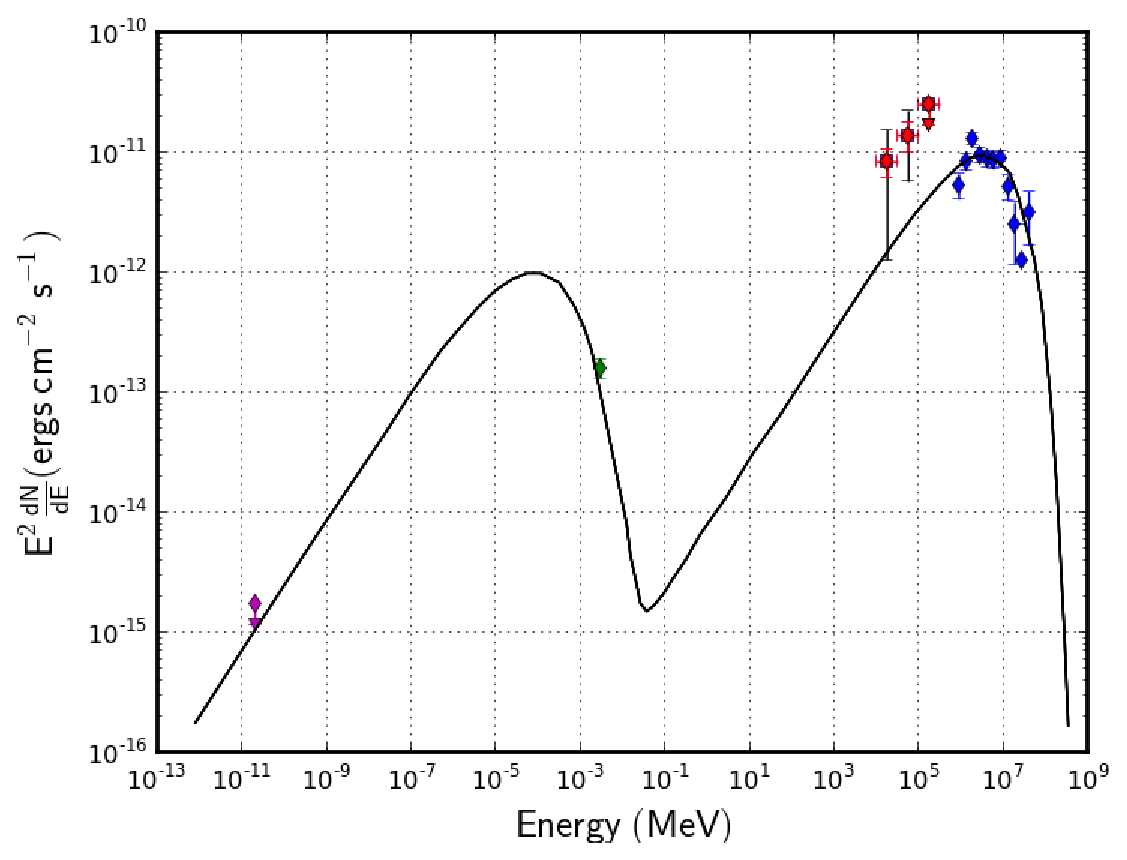
\includegraphics[width=0.60\textwidth]{figures/HESSJ1303631.eps}
\caption{SED of HESS J1303-631. The blue, green and magenta points represents HESS results, the radio data and \emph{Chandra} results \citep{dalton1303}. In the LAT energy range the red and black error bars respectively show the statistical and systematic uncertainties added in quadrature. The solid line shows the leptonic model proposed by \cite{dalton1303}.
\label{fig:hessj1303}}
\end{figure}


\begin{figure}[h!]
\centering
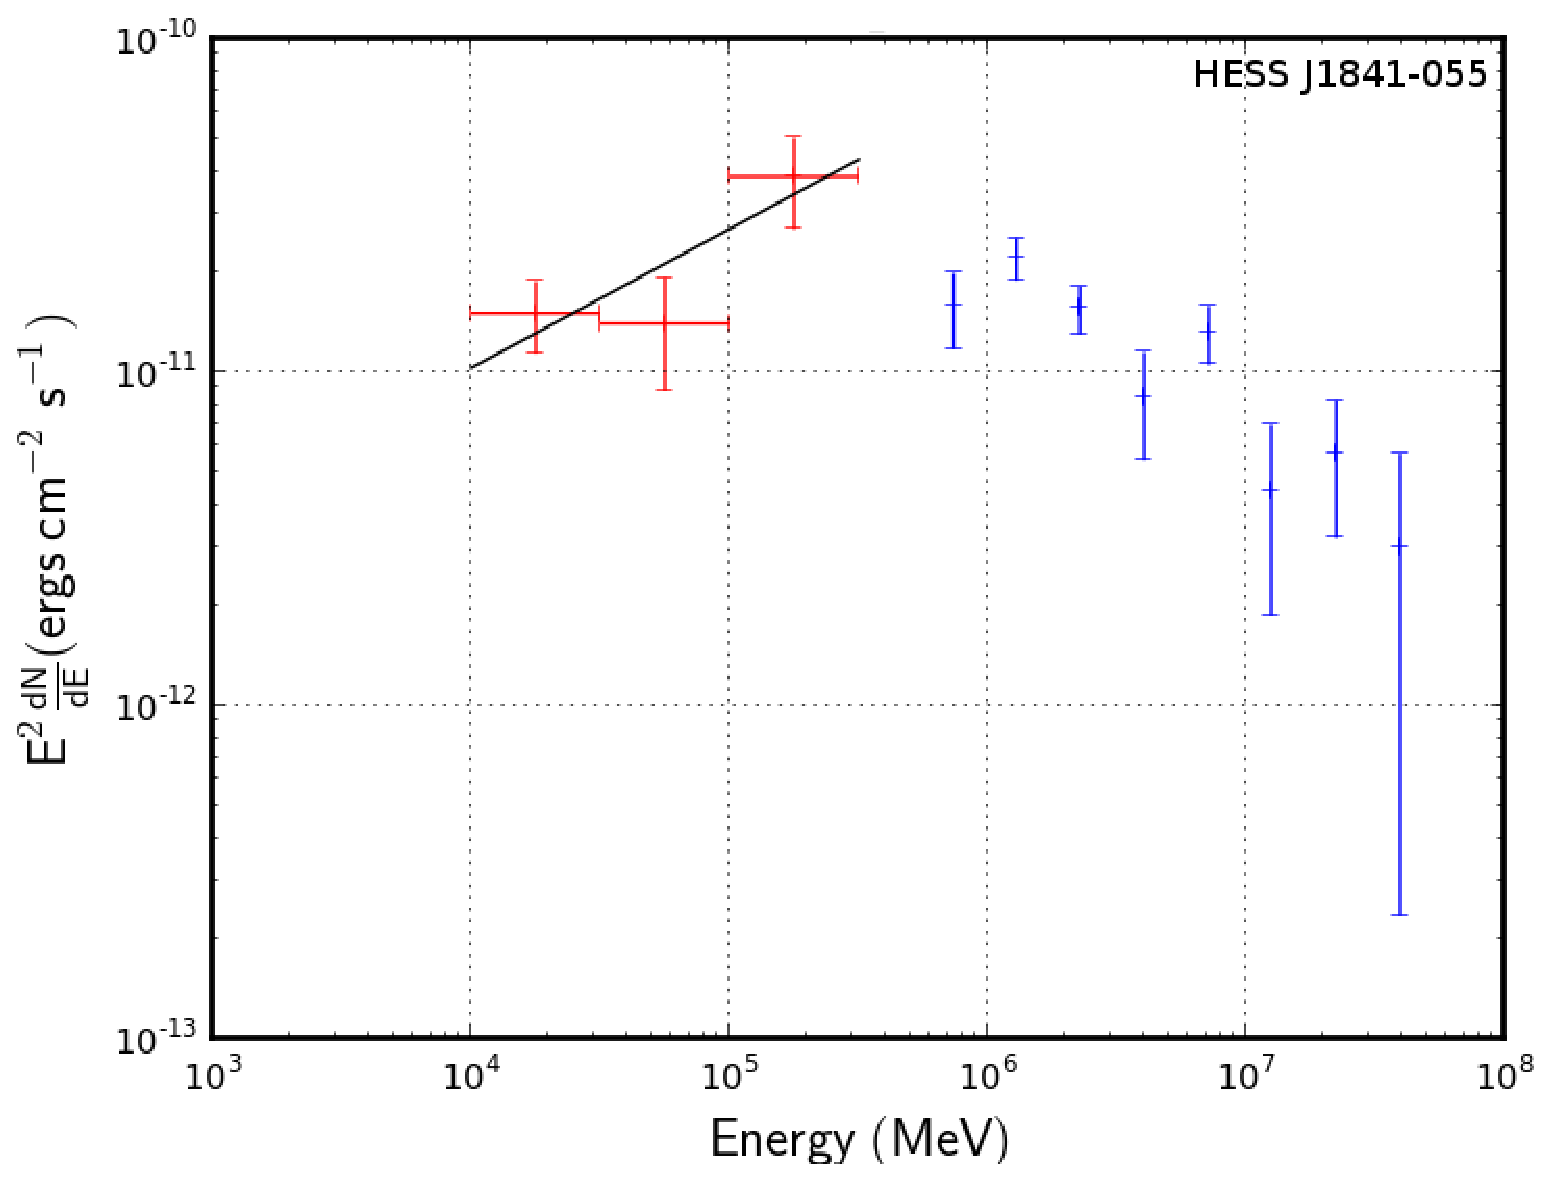
\includegraphics[width=0.60\textwidth]{figures/HESSJ1841055.eps}
\caption{SED of HESS~J1841$-$055. We reported the spectral points obtained using H.E.S.S. data in blues as well as the \emph{Fermi}-LAT spectral points in red. The red and black error bars respectively show the statistical and systematic uncertainties added in quadrature.
\label{fig:1841}}
\end{figure}

\begin{figure}[h!]
\centering
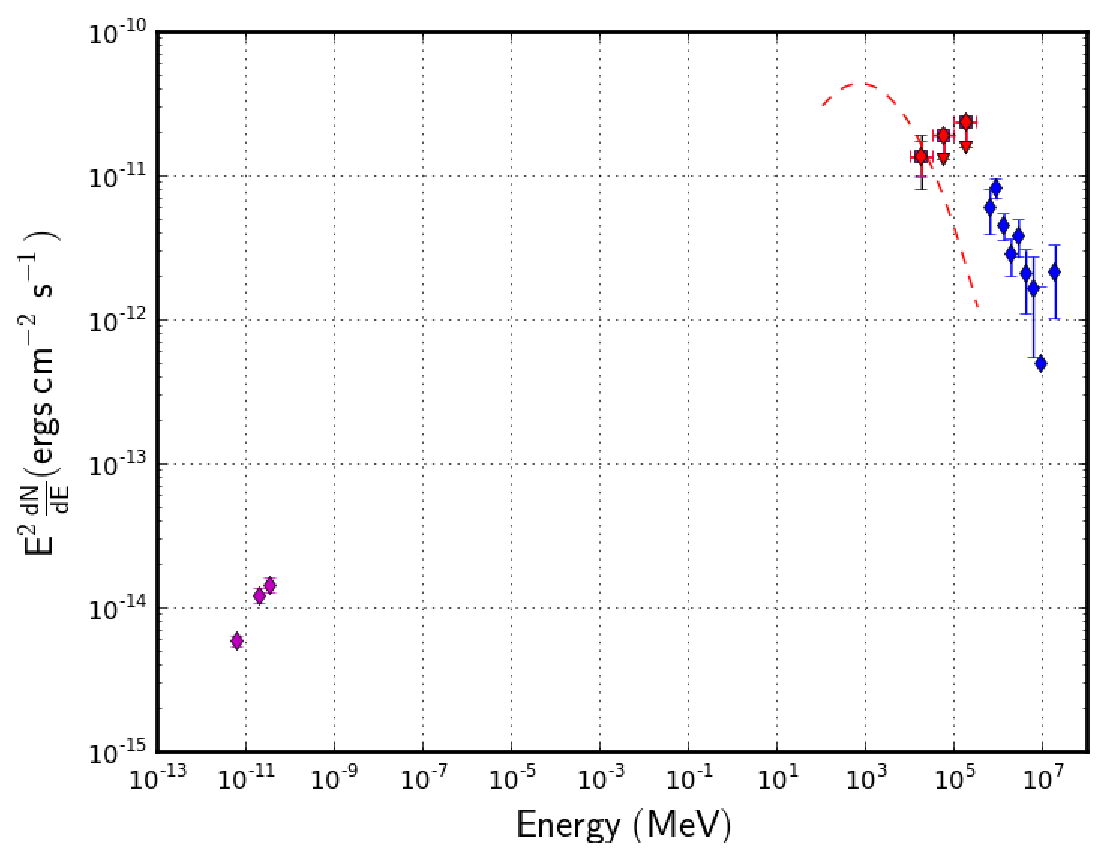
\includegraphics[width=0.60\textwidth]{figures/HESSJ1848018.eps}
\caption{SED of HESS~J1848$-$018. H.E.S.S. pectral points from \cite{chavesthesis} are presented in blue while the radio points corresponding to the W43 central cluster from \cite{2011AA...532A..92L} are indicated in magenta. Red points represent \emph{Fermi}-LAT data. The red and black error bars respectiveley show the statistical uncertainties and statistical plus systematic uncertainties added in quadrature. The red dashed line corresponds to the SED derived in \cite{2011MmSAI..82..739L} using \emph{Fermi}-LAT data and assuming a Gaussian shape of 0.3$\degr$.
\label{fig:1848}}
\end{figure}

\begin{figure}[h!]
\centering
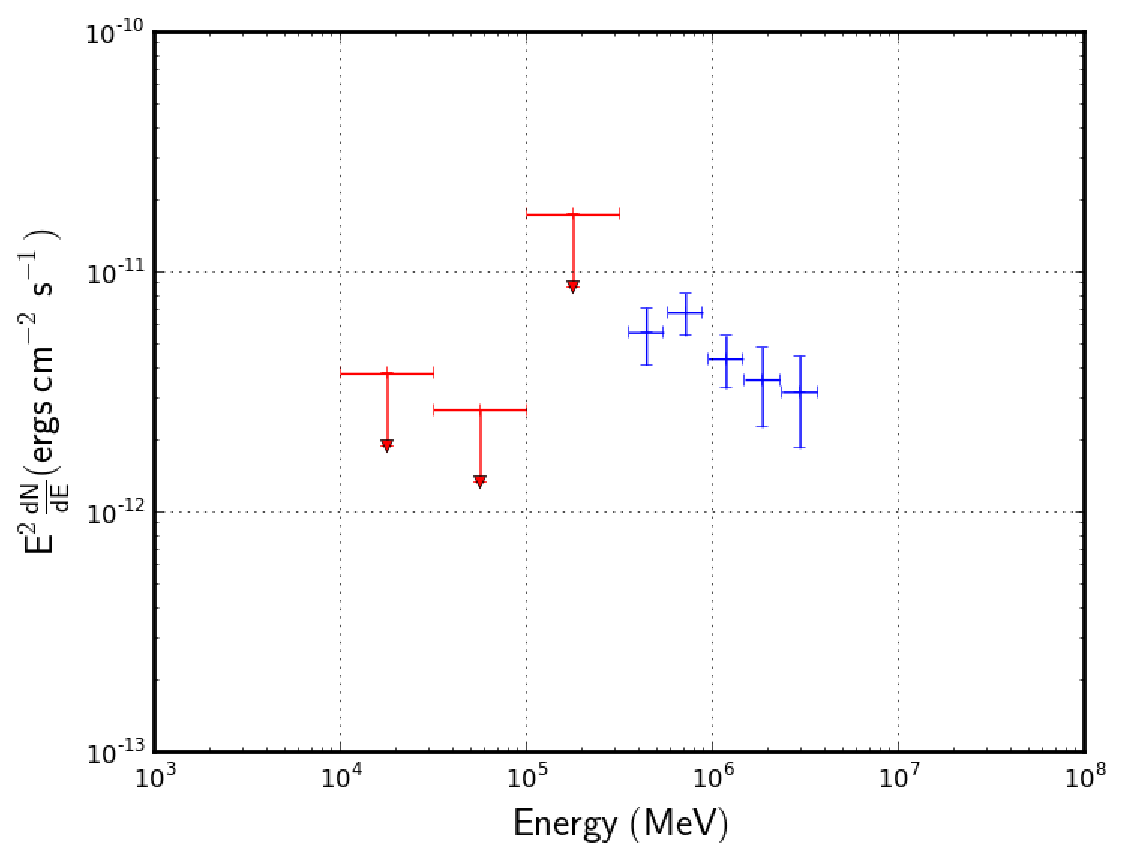
\includegraphics[width=0.60\textwidth]{figures/HESSJ1026.eps}
\caption{SED of HESS~J1026$-$582. H.E.S.S. spectral points are reported in blue while \emph{Fermi}-LAT upper limits are indicated in red. 
\label{fig:1026}}
\end{figure}

\begin{figure}[h!]
\centering
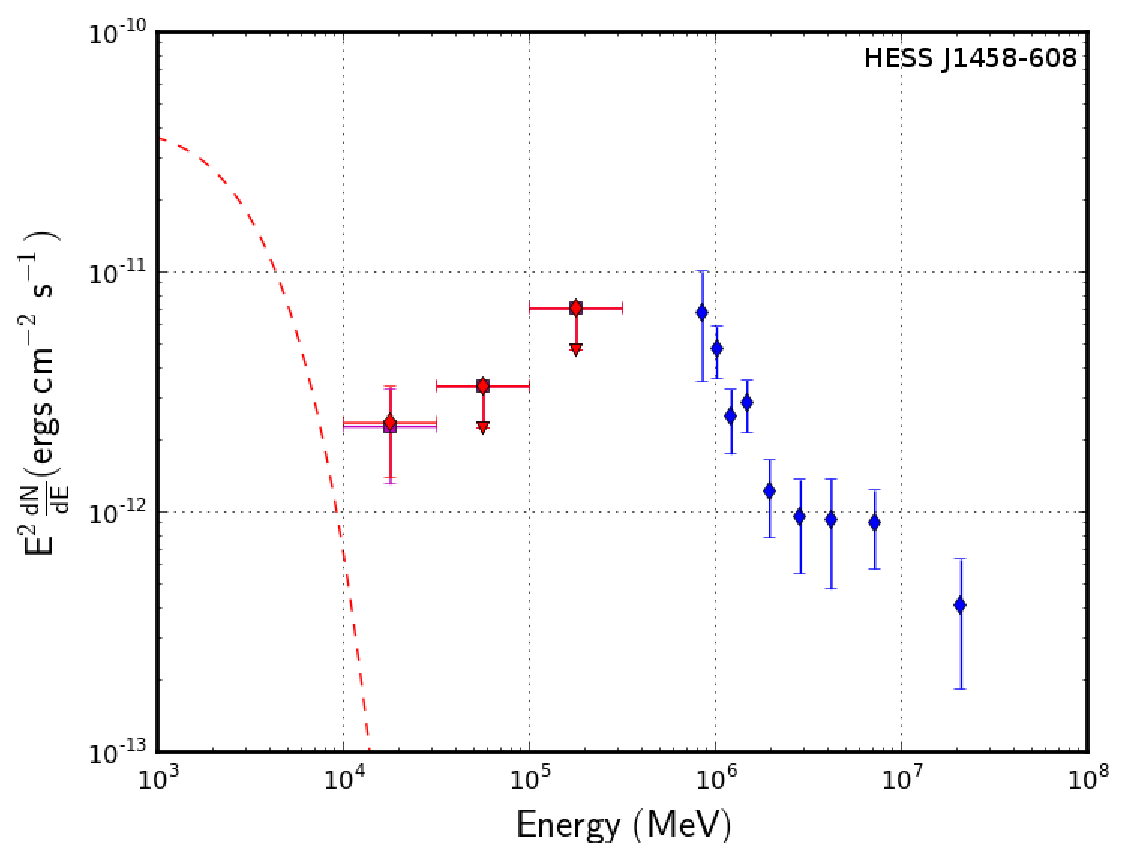
\includegraphics[width=0.60\textwidth]{figures/HESSJ1458.eps}
\caption{SED of HESS~J1458$-$608. H.E.S.S. spectral points are reported in blue while \emph{Fermi}-LAT spectral points are represented int red. The magenta points show the \emph{Fermi}-LAT points obtained once PSR~J1459$-$60 added to the model. The black error bars show the statistical and systematic uncertainties added in quadrature.
\label{fig:1458}}
\end{figure}

\begin{figure}[h!]
\centering
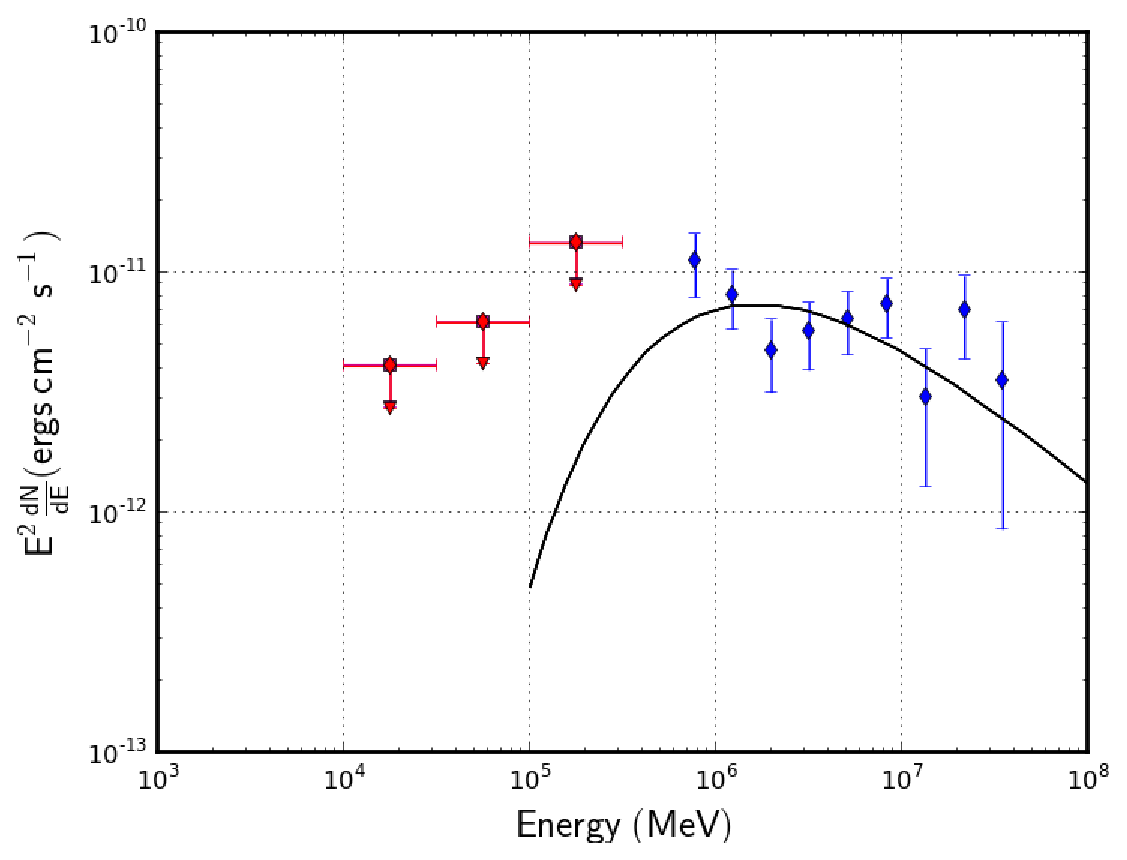
\includegraphics[width=0.60\textwidth]{figures/HESSJ1626.eps}
\caption{SED of HESS~J1626$-$490. H.E.S.S. spectral points are reported in blue while \emph{Fermi}-LAT upper-limits are indicated in red.
\label{fig:1626}}
\end{figure}

\begin{figure}[h!]
\centering
\subfigure{
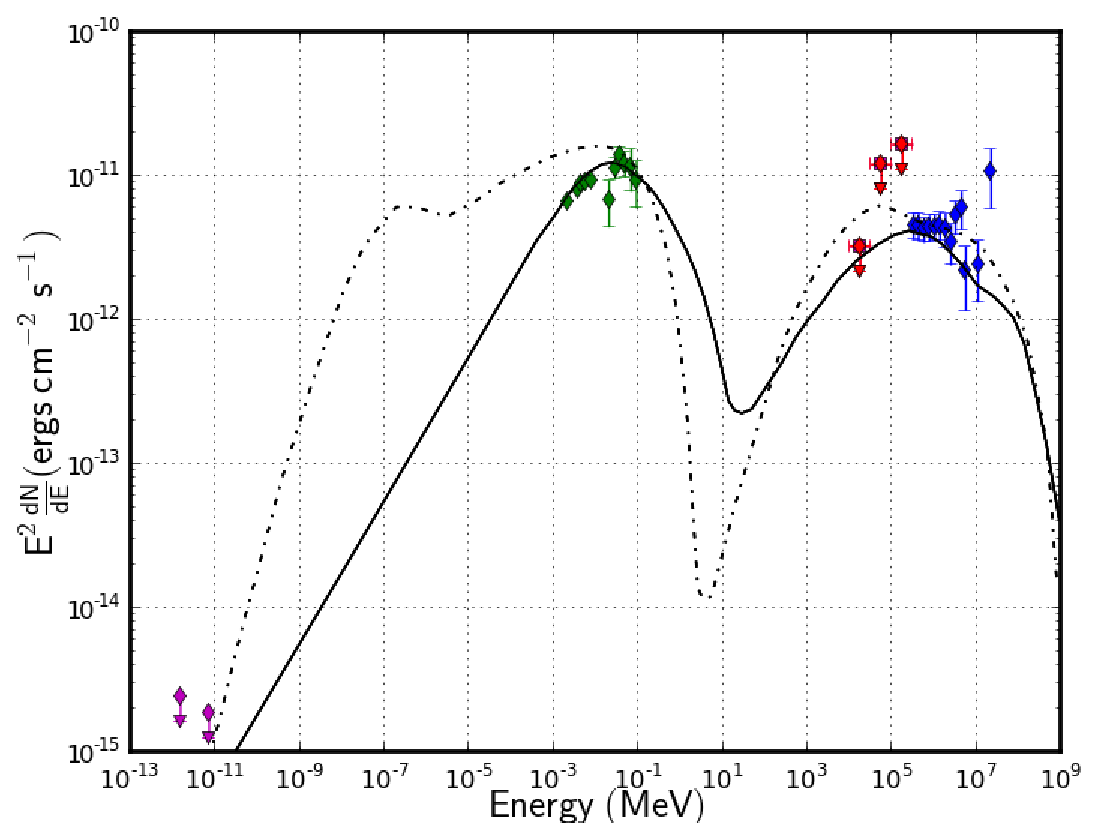
\includegraphics[width=0.60\textwidth]{figures/HESSJ1813178PWN.eps}}
\subfigure{
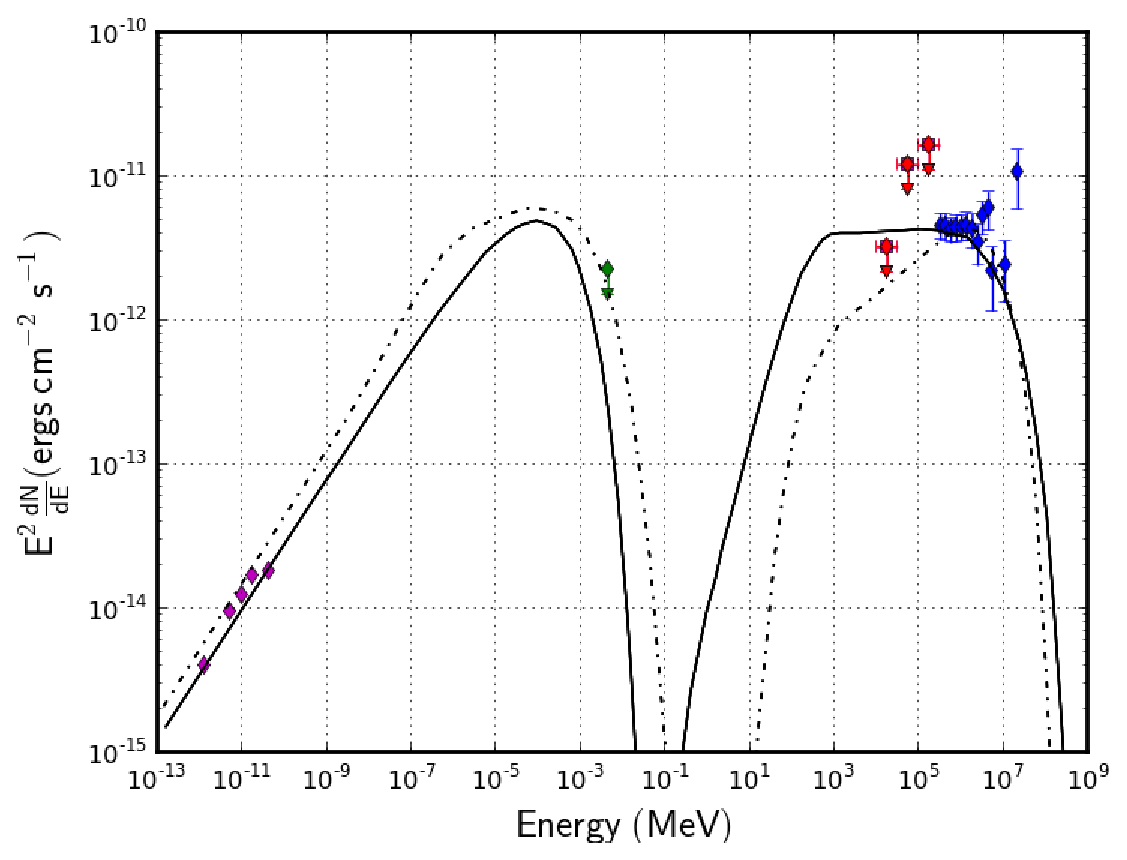
\includegraphics[width=0.60\textwidth]{figures/HESSJ1813178SNR.eps}}
\caption{SED of HESS J1813$-$178. The blue and red points show the H.E.S.S. \citep{2006ApJ...636..777A} and \emph{Fermi}-LAT spectral results. The radio data (magenta) are from VLA, Bonn, Parkes, and Nobeyama observatories \citep{2005ApJ...629L.105B}. The X-ray data are from XMM-Newton \citep{2007AA...470..249F}
and INTEGRAL \citep{2005ApJ...629L.109U}. These points were derived either for the shell of the SNR and for the core (PWN). The solid and dot dashed lines respectively correspond to the models proposed by \cite{2007AA...470..249F} and by \cite{2010ApJ...718..467F}. Top : Leptonic scenario in which the radiation is created by a PWN.  Bottom : Hadronic scenario in which the radiation is created by the SNR. 
\label{fig:hessj1813}}
\end{figure}




\clearpage

\begin{figure}[h!]
\centering
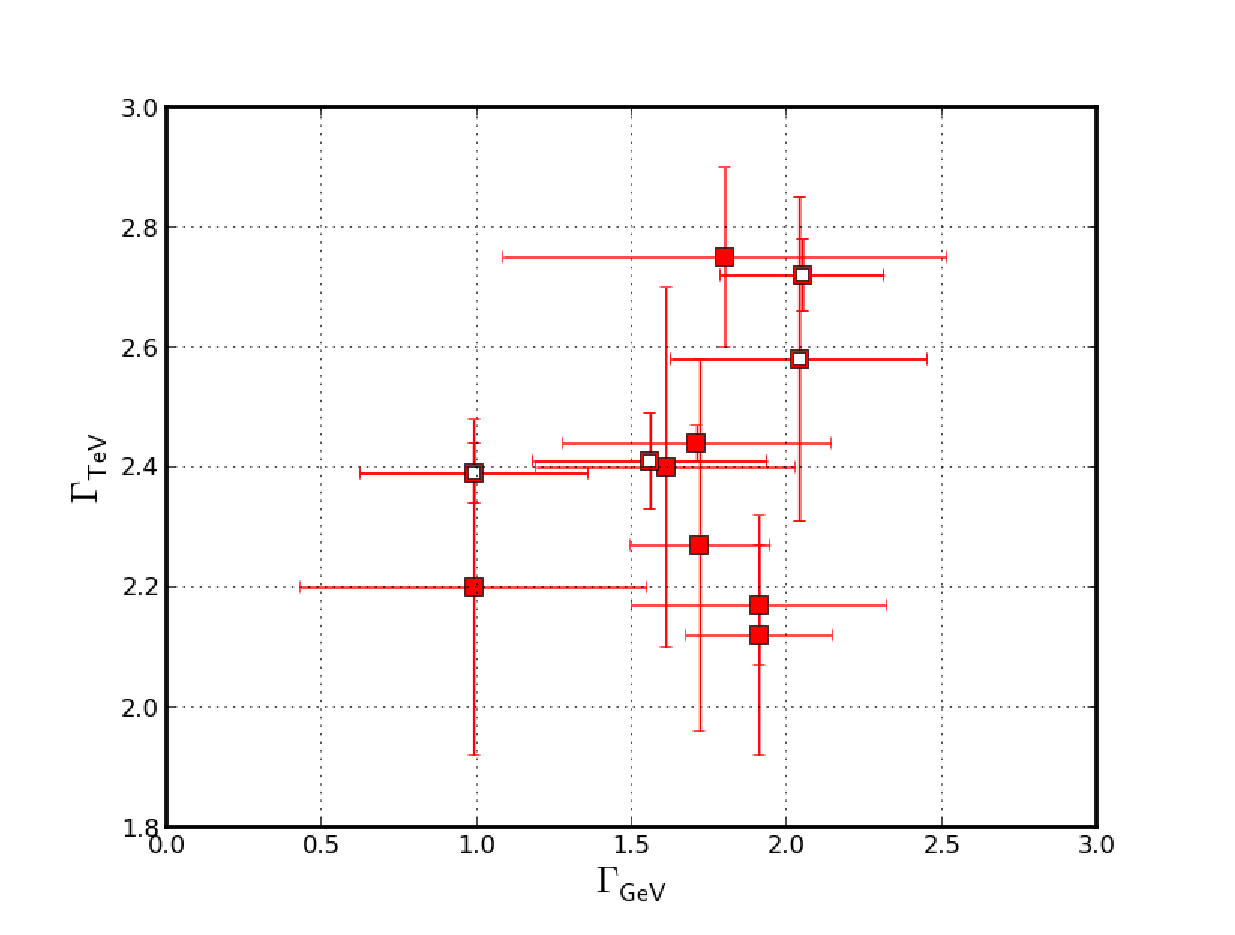
\includegraphics[width=0.5\textwidth]{figures/Gamma_GeV_Gamma_TeV.eps}
\caption{TeV spectral index as a function of the GeV spectral index for sources detected in our analysis for which the informations on the pulsar are available. These sources are summarized in Table \ref{tab:table_luminosity}. Full markers represent sources with a clear PWN association at TeV energies while hollow markers correspond to sources for which the association between TeV emission and a PWN is less clear. The dashed line corresponds to the symmetry compared to an index of 2. Pulsars summarized in Table \ref{tab:pulsarfit} are included in the model.
\label{fig:gammagamma}}
\end{figure}

\begin{figure}[h!]
\centering
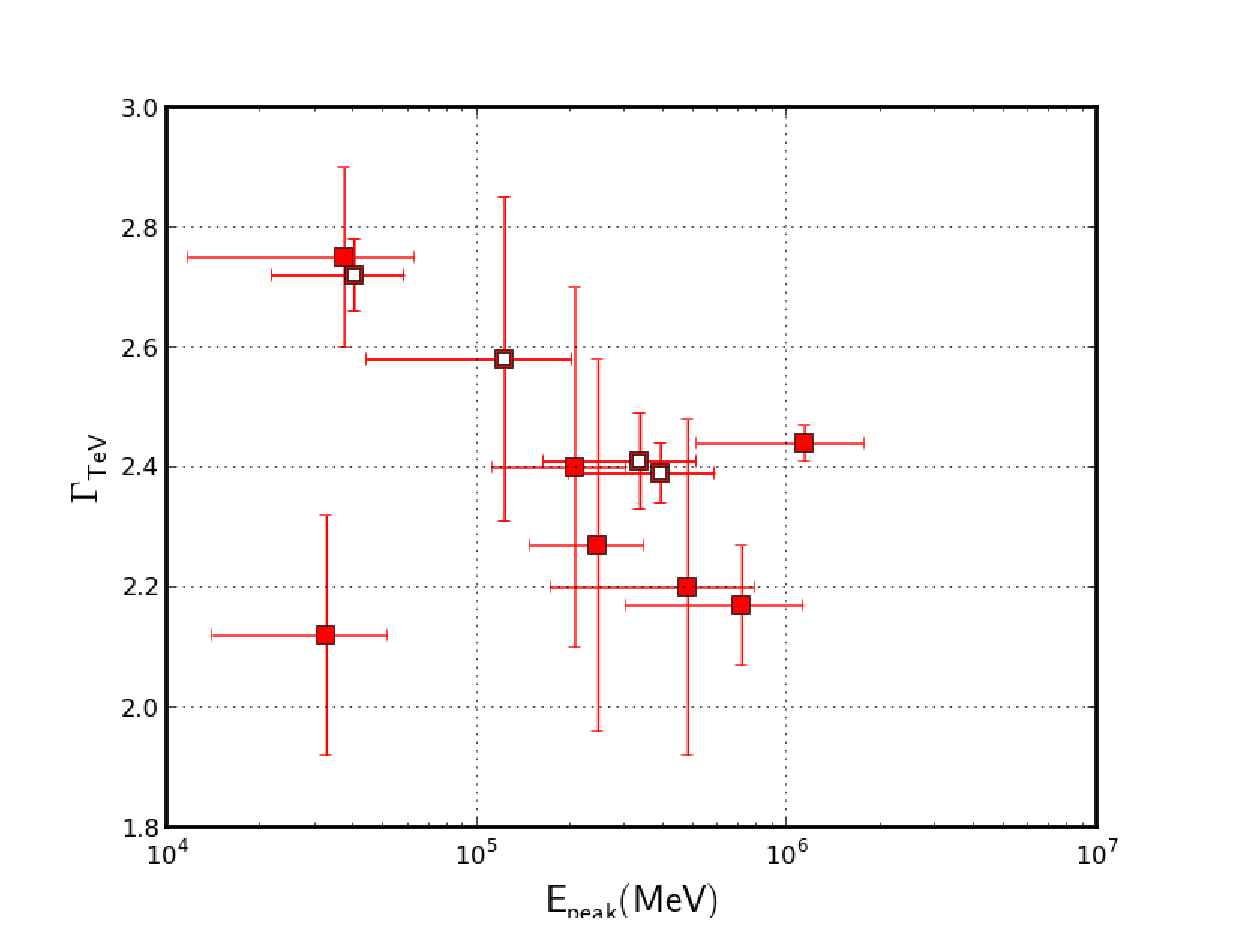
\includegraphics[width=0.5\textwidth]{figures/E_cut_vs_TeV.eps}
\caption{TeV spectral index as a function of the energy of the maximum of the IC peak for sources detected in our analysis for which the informations on the pulsar are available. These sources are summarized in Table \ref{tab:table_luminosity}. Full markers represent sources with a clear PWN association at TeV energies while hollow markers correspond to sources for which the association between TeV emission and a PWN is less clear. Pulsars summarized in Table \ref{tab:pulsarfit} are included in the model.
\label{fig:EpeakETeV}}
\end{figure}

\begin{figure}[h!]
\centering
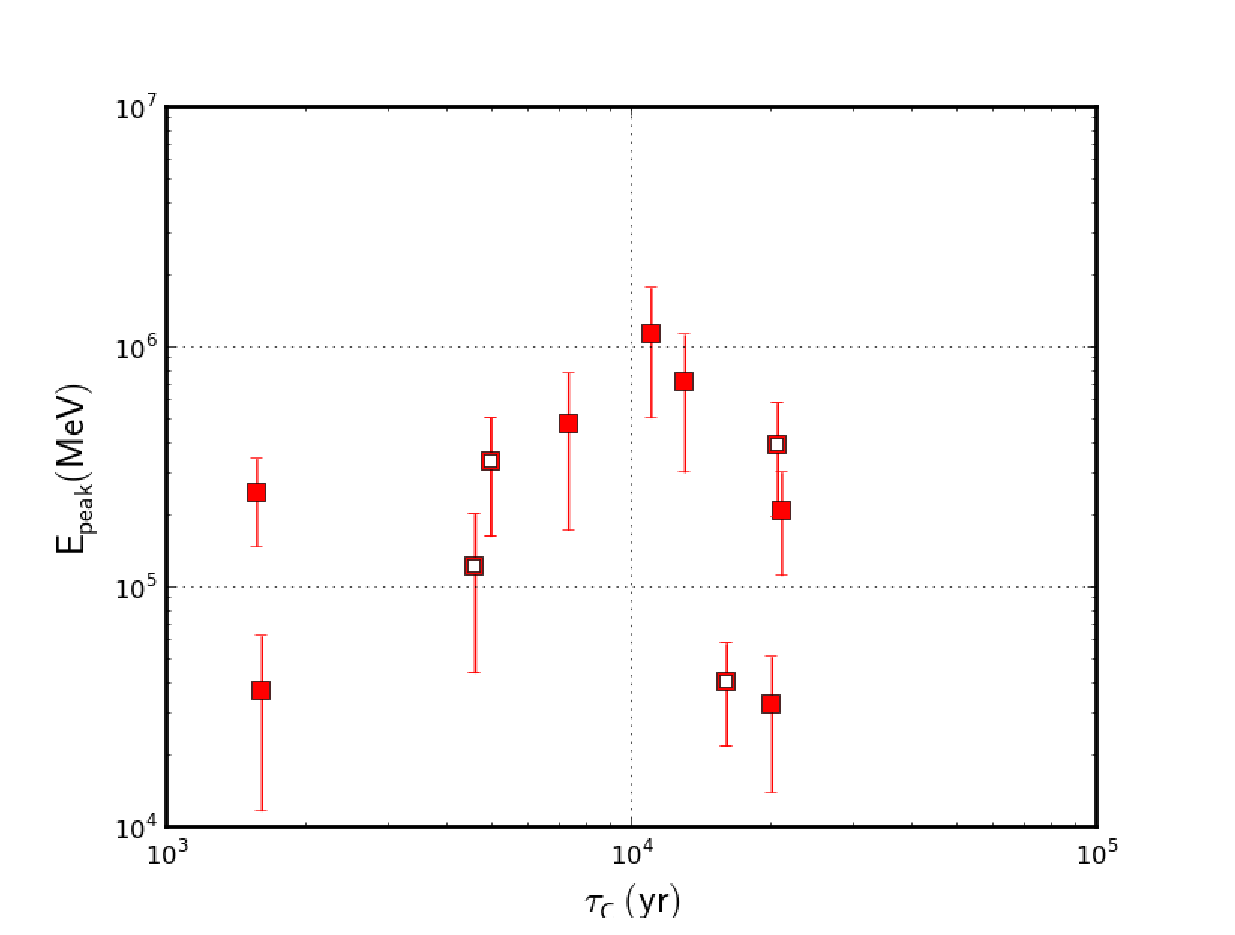
\includegraphics[width=0.5\textwidth]{figures/E_cut_vs_age.eps}
\caption{Energy of the maximum of IC peak as a function of the characteristic age of the pulsar for sources detected in our analysis for which the informations on the pulsar are available. These sources are summarized in Table \ref{tab:table_luminosity}. Full markers represent sources with a clear PWN association at TeV energies while hollow markers correspond to sources for which the association between TeV emission and a PWN is less clear. Pulsars summarized in Table \ref{tab:pulsarfit} are included in the model.
\label{fig:Epeakage}}
\end{figure}

\clearpage

\begin{figure}[h!]
\centering
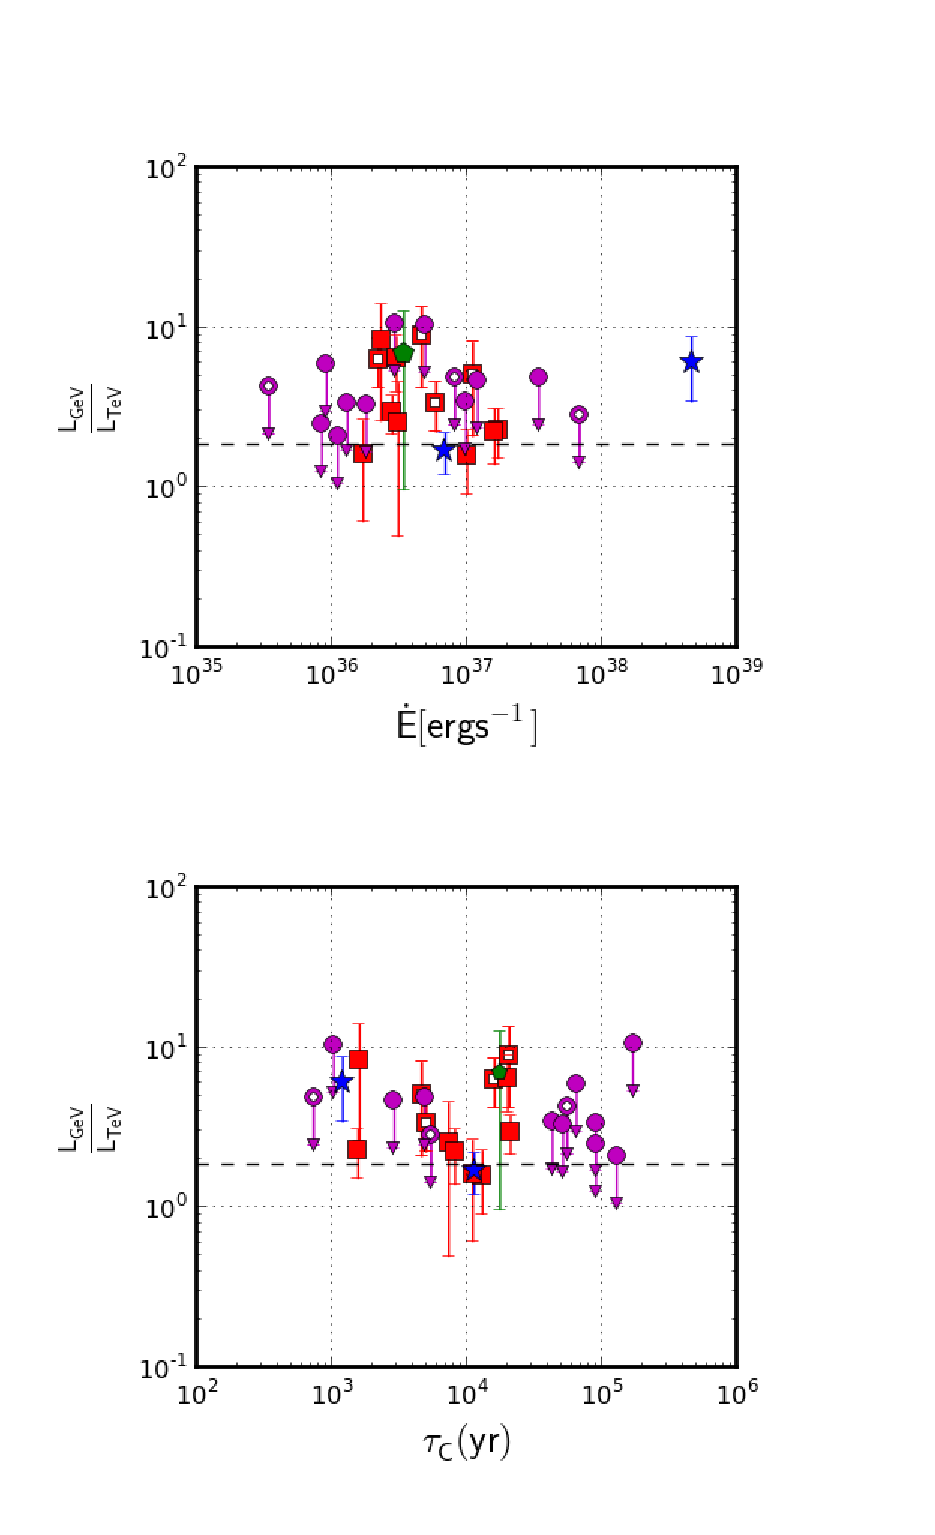
\includegraphics[width=0.5\textwidth]{figures/rapport_TeV.eps}
\caption{Ratio of luminosity of the PWN in GeV over the luminosity in TeV as a function of the pulsar spin-down power (top) and the pulsar characteristic age (bottom). Full markers correspond to sources with a clear PWN association at TeV energies while hollow markers correspond to sources for which the association between the TeV emission and a PWN is less clear. The red squares (\protect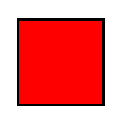
\includegraphics[scale=0.25]{figures/carrerouge.eps}) represent the sources detected at GeV energies, the magenta circles (\protect
\includegraphics[scale=0.25]{figures/rondmagenta.eps}) show the upper limits, the green pentagon (\protect
\includegraphics[scale=0.25]{figures/pentagonevert.eps}) represent the sources showing a pulsar behaviour in the energy range and the blue stars (\protect
\includegraphics[scale=0.25]{figures/etoilebleue.eps}) represent the Crab nebula and Vela-X not studied in this work. Pulsars summarized in Table \ref{tab:pulsarfit} are included in the model. The dashed line represent the mean ratio found between the GeV and the TeV flux due to the spectral shape of the IC peak.
\label{fig:rapportTeV}}
\end{figure}

\clearpage

\begin{figure}[h!]
\centering
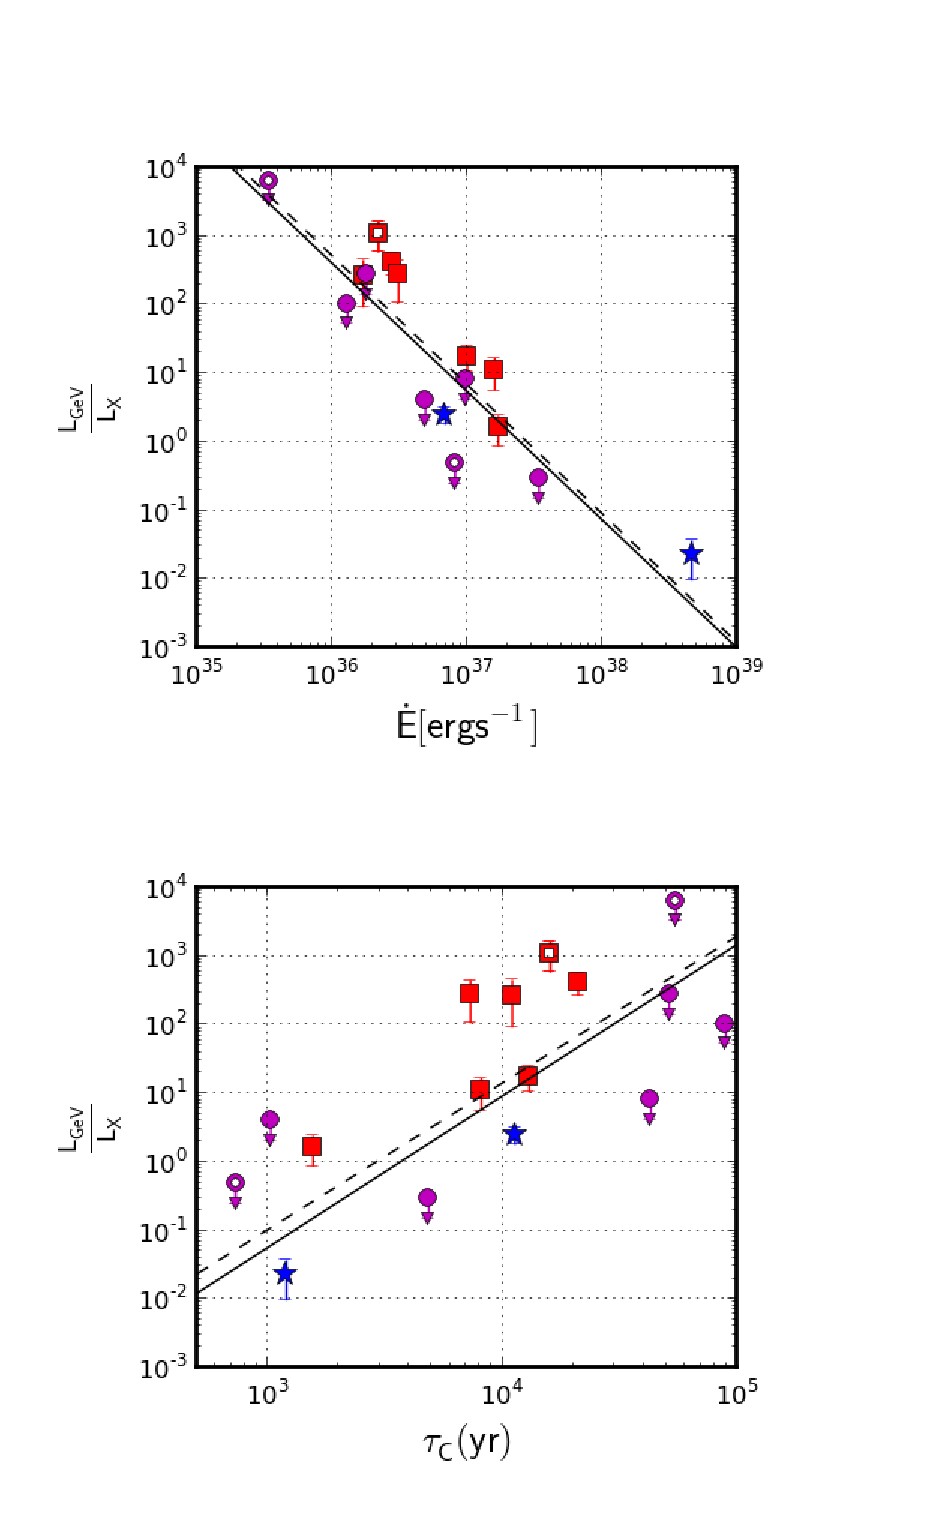
\includegraphics[width=0.5\textwidth]{figures/rapport_X.eps}
\caption{Ratio of luminosity of the PWN in GeV over the luminosity in X-rays as a function of the pulsar spin-down power (top) and the pulsar characteristic age (bottom). Full markers correspond to sources with a clear PWN association at TeV energies while hollow markers correspond to sources for which the association between the TeV emission and a PWN is less clear. The red squares (\protect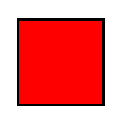
\includegraphics[scale=0.25]{figures/carrerouge.eps}) represent the sources detected at GeV energies, the magenta circles (\protect
\includegraphics[scale=0.25]{figures/rondmagenta.eps}) show the upper limits, the green pentagon (\protect
\includegraphics[scale=0.25]{figures/pentagonevert.eps}) represent the sources showing a pulsar behaviour in the energy range and the blue stars (\protect
\includegraphics[scale=0.25]{figures/etoilebleue.eps}) represent the Crab nebula and Vela-X not studied in this work. Pulsars summarized in Table \ref{tab:pulsarfit} are included in the model. The dashed and solid lines represent respectively the relations derived in \cite{2009ApJ...694...12M} multiplied by $\bar{R}$ for the whole sample of sources and for the sources clearly identify to PWNe.
\label{fig:rapportX}}
\end{figure}

\clearpage

\begin{figure}[h!]
\centering
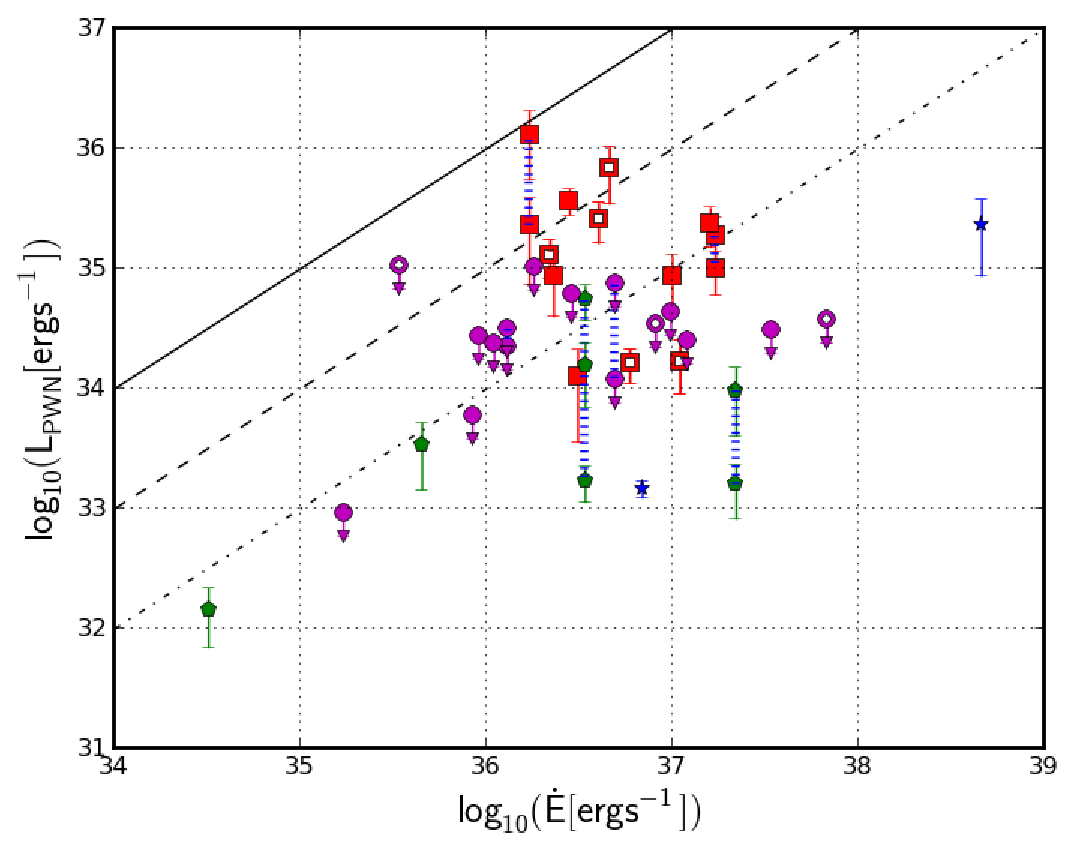
\includegraphics[]{figures/dotelpwn.eps}
\caption{Luminosity of the PWN as a function of the pulsar spin-down power. Full markers correspond to sources with a clear PWN association at TeV energies while hollow markers correspond to sources for which the association between the TeV emission and a PWN is less clear. The red squares (\protect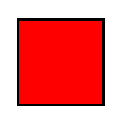
\includegraphics[scale=0.25]{figures/carrerouge.eps}) represent the sources detected at GeV energies, the magenta circles (\protect
\includegraphics[scale=0.25]{figures/rondmagenta.eps}) show the upper limits, the green pentagon (\protect
\includegraphics[scale=0.25]{figures/pentagonevert.eps}) represent the sources showing a pulsar behaviour in the energy range and the blue stars (\protect
\includegraphics[scale=0.25]{figures/etoilebleue.eps}) represent the Crab nebula and Vela-X not studied in this work. Sources with two distances estimates have two markers connected with a dotted blue line. Pulsars summarized in Table \ref{tab:pulsarfit} are included in the model. 
\label{fig:dotelpwn}}
\end{figure}

\clearpage


\clearpage
\appendix
\renewcommand{\thefigure}{A-\arabic{figure}}
\setcounter{figure}{0}
\appendix


\end{document}
